\documentclass{article}
% Преамбула сборника. Подключается из main.tex и из сборок отдельных глав.
\usepackage[T2A]{fontenc}     % кодировка шрифтов
\usepackage[utf8]{inputenc}   % кодировка исходного файла
\usepackage[russian]{babel}   % поддержка русского
\usepackage[a4paper,margin=1.2cm]{geometry}
\usepackage{amsthm, amssymb}
\usepackage{amsmath}
\usepackage{float}
\usepackage{graphicx} % Required for inserting images
% Иллюстрации разложены по происхождению, но в \includegraphics по-прежнему
% указывается только имя файла.
\graphicspath{{figures/book/}{figures/own/}}
\usepackage{caption}
\usepackage{wrapfig}
\usepackage{subcaption}
\usepackage{tikz}
\usetikzlibrary{positioning,arrows.meta}
% --- навигация по документу -------------------------------------------------
% hyperref загружается до algorithm2e: обратный порядок ломает нумерацию
% строк в окружении algorithm.
\usepackage[unicode, hidelinks]{hyperref}
\hypersetup{
    bookmarksnumbered = true,
    bookmarksopen     = true,
    pdftitle          = {Ответы к книге «Обучение с подкреплением», Саттон и Барто},
    pdfsubject        = {Решения упражнений},
}

\usepackage[ruled, linesnumbered]{algorithm2e}

\captionsetup{labelformat=empty,hypcap=false}
\emergencystretch=3em
\hfuzz=30pt
\hbadness=10000
\sloppy

\renewcommand{\qedsymbol}{$\blacksquare$}

\newenvironment{solution}
  {\begin{proof}[Решение]}
  {\end{proof}}


\title{Ответы к книге "Обучение с подкреплением" Саттон, Барто}
\author{}
\date{}


% Раскомментируйте, чтобы быстро пересобрать одну главу:
% \includeonly{chapters/ch06}

\begin{document}
\maketitle
\tableofcontents
\section{Глава 1. Введение}
\subsection{Упражнение 1.1. Игра с самим собой(с.38)}
Предположим, что вместо игры со случайным противником описанный выше алгоритм обучения с подкреплением играет против себя самого, и обе стороны обучаются. Как вы думаете, что произойдет в таком случае? Обучится ли игрок другой стратегии выбора ходов?
\begin{solution}
    Заметим, что в таком случае мы имеем дело с нестационарной средой, в которой вероятность перехода в состояние $s'$ из состояния $s$ зависит от политики противника. \\
    Обратимся к словам автора на странице 36: "Если размер шага не уменьшается со временем до нуля, то этот игрок будет хорошо играть и с противниками, которые медленно изменяют манеру игры."\ Это означает, что если потребовать определенные условия на коэффициент $\alpha$, то такой способ обучения приведет к более универсальной стратегии, но лишь в "практическом"\ смысле, а не строгом математическом. О сходимости к оптимальной стратегии тут речь не идет, потому что классические результаты TD-обучения требуют стационарности среды.
\end{solution}

\subsection{Упражнение 1.2. Симметрии(c.38)}
Многие позиции в крестиках-ноликах выглядят различными, но на самом деле отличаются только симметрией. Как можно изменить описанный выше процесс обучения, чтобы воспользоваться этим фактом? Как это изменение могло бы улучшить процесс обучения? А теперь подумайте еще раз. Предположим, что противник не пользуется преимуществами симметрии. Должны ли тогда это делать мы? И верно ли, что позиции, совпадающие с точностью до симметрии, имеют одну и ту же ценность? 
\begin{solution}
    Сначала рассмотрим случай, когда оба игрока придерживаются принципа симметрии. В таком случае логично будет сгруппировать положения доски относительно некоторых канонических состояний. И обновлять ценности следует одновременно по всем эквивалентным позициям. Это приводит к меньшему количеству уникальных состояний, более быстрому обучению, более стабильным оценкам $V(s)$. \\
    Если же противник не пользуется симметрией, то совпадающие позиции перестают иметь одну и ту же ценность, потому что два симметричных состояния могут привести к разным распределениям будущих ходов. И, следовательно, пользоваться симметрией нам теперь невыгодно, так как предложенный алгоритм основан на значении $V(s)$.
\end{solution}

\subsection{Упражнение 1.3. Жадная игра(с.39)}
Предположим, что обучающийся с подкреплением игрок жадный, т. е. всегда выбирает ход, который переводит его в позицию с наивысшим рейтингом. Мог бы он научиться играть лучше нежадного игрока? Или хуже? Какие проблемы могли бы возникнуть?
\begin{solution}
    Абсолютное отсутствие исследования - ключевой недостаток жадного подхода. Теоретически, агент может научиться играть лучше нежадного игрока, но по чистой случайности, в искусственных случаях. В практических задачах это никогда не встретится. Исключение возможности исследовать пространство решений приводит к застреванию в локальных областях, далеко не оптимальным стратегиям. Объясняется это тем, что игрок навсегда закрепляет ошибочные ранние оценки. Ещё одна проблема - зависимость от начальных условий.
\end{solution}

\subsection{Упражнение 1.4. Обучение на результатах разведки(с.39)}
Предположим, что обучение подвергается обновлению после любого хода, включая разведочные. Если со временем размер шага уменьшается подходящим образом (но не уменьшается стремление к исследованию), то ценности состояний будут сходиться к другому набору вероятностей. Что концептуально представляют собой два набора вероятностей, вычисленных, когда мы обучаемся и не обучаемся на разведочных ходах? В предположении, что мы продолжаем совершать разведочные ходы, какой набор вероятностей предпочтительнее обучить? Какой принесет больше выигрышей?
\begin{solution}
    Метод без обучения на разведочных данных вычисляет ценности оптимальной политики. Это идеальные ожидаемые выигрыши, если бы агент всегда действовал оптимально, без исследовательских шагов. Но при этом агент совершает случайные действия. Это означает, что найденные ценности соответствуют не той политике, которой придерживается игрок, а идеальному случаю. \\
    Обновление ценностей на разведочных ходах соответствует реальному поведению агента, поэтому логичнее их учитывать, чтобы вычисленные ценности соответствовали действительности. При достаточном обучении именно такой подход принесет больше выигрышей по этой же причине, несмотря на выполнение следующего неравенства:
    \[v_*(s) \ge v_\pi(s) \qquad \forall s \in S,\]
    где $v_*(s)$ - ценность состояния $s$ при оптимальной политике, а $v_\pi(s)$ - ценность состояния $s$ при политике, включающей разведочные ходы.
\end{solution}

\subsection{Упражнение 1.5. Другие улучшения(с.39)}
Можете ли вы предложить иные способы улучшить игрока, обучающегося с подкреплением? Можете ли вы придумать лучший способ решения задачи об игре в крестики-нолики в том виде, в котором она поставлена?
\begin{solution}
   Кроме улучшений, предложенных в предыдущих упражнениях, я могу предложить следующие:
   \begin{itemize}
       \item Обновление не только предыдущего шага, но и всей истории по правилу
        \[
            V(s_{t-k}) \leftarrow V(s_{t-k}) 
            + \alpha_k \bigl( V(s_{t+1}) - V(s_{t-k}) \bigr),
            \quad k=\overline{0,t} \quad\alpha_k \downarrow \text{по } k
        \]
       \item Постепенное уменьшение вероятности исследования с течением времени улучшает итоговую игру.
   \end{itemize}
   Крестики-нолики являются антагонистической игрой(выигрыш одного равен проигрышу другого) с полной информацией. Более того, множество состояний конечно и невелико. Поэтому к игре применимы классические подходы из теории игр, исследующие минимаксные стратегии.
\end{solution}


\newpage
\part{Табличные методы решения}

\section{Глава 2. Многорукие бандиты}
\subsection{Упражнение 2.1(c. 54)}
Рассмотрим $\varepsilon$-жадный выбор действия для случая двух действий и $\varepsilon = 0.5$. Чему равна вероятность выбора жадного действия? 
\begin{solution}
    Для $\varepsilon$-жадной стратегии:
    \begin{itemize}
        \item с вероятностью $1-\varepsilon$ выбирается жадное действие.
        \item с вероятностью $\varepsilon$ выбирается случайное действие.
    \end{itemize}
    Поэтому $\mathbb{P}(\text{жадное}) = 1-\varepsilon+\varepsilon \cdot \frac{1}{2}=0.75$
\end{solution}

\subsection{Упражнение 2.2. Пример бандита(c. 57)}
Рассмотрим задачу о $k$-руком бандите с $k = 4$ действиями, обозначенными $1, 2, 3, 4$. Разберем применение к этой задаче алгоритма бандита с $\varepsilon$-жадным выбором действия, выборочным усреднением оценок ценности действий и начальными оценками $Q_1(a) = 0 \ \text{для} \ \forall a$. Предположим,
что начало последовательности действий и вознаграждений выглядит так: $A_1 = 1,
R_1 = 1, A_2 = 2, R_2 = -1, A_3 = 2, R_3 = -2, A_4 = 2, R_4 = 2, A_5 = 3, R_5 = 0$. На некоторых из этих временных шагов мог иметь место $\varepsilon$-случай, т.е. действие выбирается случайным образом. На каких шагах так оно заведомо и было? На каких шагах это могло случиться, а могло и не случиться?
\begin{solution} 
    Рассмотрим таблицу, где $Q_t(i), \ i=\overline{1,4}$ - значения оценок истинной ценности до выбора действия $A_t$:
    \renewcommand{\arraystretch}{1.3}
    \begin{table}[H]
    \centering
    \begin{tabular}{|c|c|c|c|c|c|c|c|}
    \hline
    $t$ 
    & $A_t$ 
    & $R_t$ 
    & $Q_t(1)$ 
    & $Q_t(2)$ 
    & $Q_t(3)$ 
    & $Q_t(4)$ 
    & $\varepsilon$-случай \\ \hline
    1 & 1 & 1 
    & 0 
    & 0 
    & 0 
    & 0 
    & мог быть / мог не быть \\
    \hline
    
    2 & 2 & $-1$ 
    & 1 
    & 0 
    & 0 
    & 0 
    & был заведомо \\
    \hline
    
    3 & 2 & $-2$ 
    & 1 
    & $-1$ 
    & 0 
    & 0 
    & был заведомо \\
    \hline
    
    4 & 2 & 2 
    & 1 
    & $-\frac{3}{2}$ 
    & 0 
    & 0 
    & был заведомо \\
    \hline
    
    5 & 3 & 0 
    & 1 
    & $-\tfrac{1}{3}$ 
    & 0 
    & 0 
    & был заведомо \\
    \hline
    
    6 & - & -
    & 1
    & $-\tfrac{1}{3}$ 
    & 0 
    & 0 
    & - \\
    \hline
    \end{tabular}
    \end{table}
\end{solution}

\subsection{Упражнение 2.3(с. 57)}
Глядя на рис. 2.2, можете ли вы сказать, какой метод будет работать лучше других в долгосрочной перспективе в терминах суммарного вознаграждения и вероятности выбора оптимального действия? Насколько лучше он будет? Выразите свой ответ количественно.
\begin{figure}
    \centering
    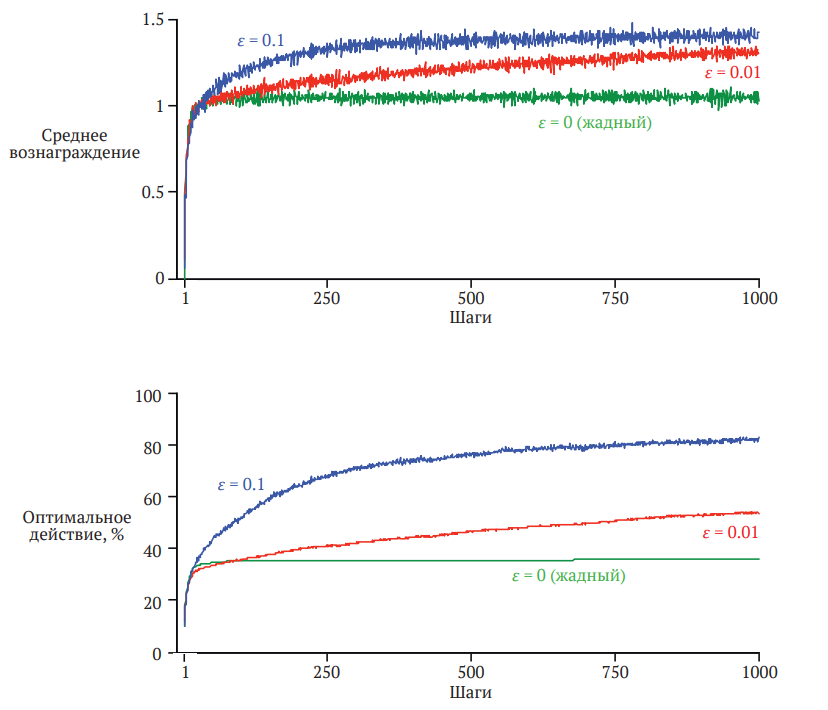
\includegraphics[width=1\linewidth]{fig_2_2.png}
    \caption{Рис. 2.2. Среднее качество $\varepsilon$-жадных методов оценки действий на 10-руком испытательном стенде. Данные получены усреднением по 2000 прогонов с разными
    задачами о бандите. Во всех методах использовалось выборочное усреднение оценок ценности действий}
\end{figure}
\begin{solution}
    \textbf{Вероятность.}
    Учтем, что при $\varepsilon > 0$ в долгосрочной перспективе оптимальное действие становится известно. Жадный алгоритм($\varepsilon = 0$) застревает в неверных шагах. Для вероятности выбора оптимального действия справедлива формула:
    \[\mathbb{P}(A_t=a^*) = (1 - \varepsilon) + \varepsilon \cdot \frac{1}{10}\]
    Тогда для
    \begin{itemize}
        \item $\varepsilon = 0.01: \quad \mathbb{P}(A_t=a^*) = 0.991$
        \item $\varepsilon = 0.1: \quad \mathbb{P}(A_t=a^*) = 0.91$
    \end{itemize}
    
    \textbf{Вознаграждение.} 
    Рассмотрим один временной шаг и запишем данные нам условия:
    \[q_*(1), \dots,q_*(10) \sim\mathcal N(0,1)\]
    \[R_t \mid (A_t = a) \sim\mathcal N(q_*(a),1)\]
    Используем закон полного математического ожидания:
    \[\mathbb{E}(R_t) = \mathbb{E}(\mathbb{E}(R_t \mid A_t)) = \mathbb{E}(q_*(A_t)),\]
    где ожидание берется и по $q_*$, и по случайности выбора действия $A_t$. \\
    Продолжая расписывать правую часть равенства, получаем
    \[\mathbb{E}(q_*(A_t)) = (1 - \varepsilon) \cdot \mathbb{E}(q_{max}) + 
    \varepsilon \cdot \mathbb{E}(\overline{q}),\]
    где $\mathbb{E}(\overline{q}) = \mathbb{E}_q(\frac{1}{10}\sum_{a=1}^{10}q_*(a)) = 0$ по условию задачи, а $q_{max} = \max_{a=1,\dots,10}q_*(a)$.\\
    В учебнике упоминается, что $\mathbb{E}(q_{max}) \approx 1.55$.\\
    Итого, мы получили:
    \[\mathbb{E}(R_t) \approx (1 - \varepsilon)\cdot1.55\]
    Тогда для
    \begin{itemize}
        \item $\varepsilon = 0.01: \quad \mathbb{E}(R_t) \approx 1.5345$
        \item $\varepsilon = 0.1: \quad \mathbb{E}(R_t) \approx 1.395$
    \end{itemize}
    Получается, что в среднем на одном временном шаге $\varepsilon = 0.01$ дает на $0.1395$ единиц вознаграждения больше, чем $\varepsilon = 0.1$.
\end{solution}

\subsection{Упражнение 2.4(с. 60)}
Если размеры шагов $\alpha_n$ непостоянны, то оценка $Q_n$ является взвешенным средним ранее полученных вознаграждений с весами, отличными от представленных в формуле (2.6). По аналогии с (2.6) выразите вес каждого предшествующего вознаграждения в терминах последовательности размеров шагов в общем случае. 
\begin{equation}
Q_{n+1} = (1 - \alpha)^n \cdot Q_1 + \sum_{i=1}^{n}\alpha \cdot (1-\alpha)^{n-i} \cdot R_i
\tag{2.6}
\end{equation}
\begin{solution}
    Начнём с общего правила обновления:
\[
Q_{n+1}
= Q_n + \alpha_n (R_n - Q_n)
= (1-\alpha_n) Q_n + \alpha_n R_n .
\]

Подставим выражение для $Q_n$:
\[
Q_n
= (1-\alpha_{n-1}) Q_{n-1} + \alpha_{n-1} R_{n-1}.
\]

Тогда
\[
Q_{n+1}
= (1-\alpha_n)\bigl[(1-\alpha_{n-1}) Q_{n-1}
+ \alpha_{n-1} R_{n-1}\bigr]
+ \alpha_n R_n.
\]

Раскрывая скобки, получаем:
\[
Q_{n+1}
= (1-\alpha_n)(1-\alpha_{n-1}) Q_{n-1}
+ (1-\alpha_n)\alpha_{n-1} R_{n-1}
+ \alpha_n R_n.
\]

Продолжая подстановку рекурсивно, имеем:
\begin{equation}
Q_{n+1}
= \Bigl(\prod_{i=1}^{n} (1-\alpha_i)\Bigr) Q_1
+ \sum_{k=1}^{n}
\Bigl(\alpha_k \prod_{i=k+1}^{n} (1-\alpha_i)\Bigr) R_k
\tag{$*$}
\end{equation}


Следовательно, вес вознаграждения $R_k$ равен:
\[
w_k^{(n)}
= \alpha_k \prod_{i=k+1}^{n} (1-\alpha_i),
\qquad k=1,\dots,n.
\]
\end{solution}

\subsection{Упражнение 2.5(с. 60)}
Спланируйте и поставьте эксперимент, демонстрирующий трудности, с которыми сталкиваются методы выборочного среднего в нестационарных задачах. Используйте модифицированную версию
$10$-рукого испытательного стенда, в которой все $q^*(a)$ вначале равны, а затем вычисляются путем независимых случайных блужданий (скажем, путем прибавления нормально распределенного приращения со средним $0$ и стандартным отклонением $0.01$ ко всем $q^*(a)$ на каждом шаге). Постройте графики, как на рис.2.2, для метода ценности действий, в  котором используются инкрементно вычисляемые выборочные средние, и еще одного метода, в котором размер шага постоянный, $\alpha = 0.1$. Положите $\varepsilon = 0.1$, а количество шагов возьмите большим, скажем $10 000$.
\begin{solution}
    \textbf{Код смотри в отдельном файле репозитория.}
    \begin{figure}[H]
        \centering
        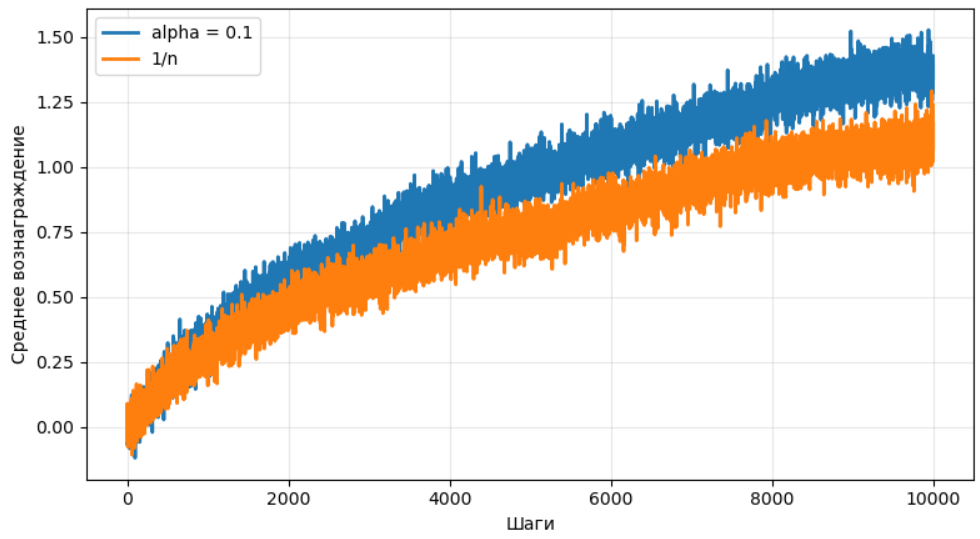
\includegraphics[width=1\linewidth]{fig_2_5_sol_1.png}
    \end{figure}
    \begin{figure}[H]
        \centering
        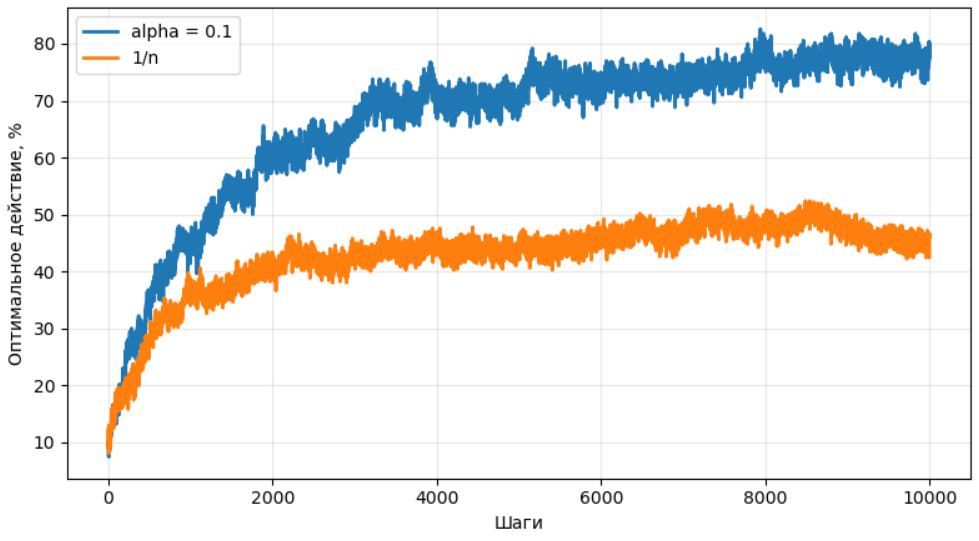
\includegraphics[width=1\linewidth]{fig_2_5_sol_2.png}
    \end{figure}
\end{solution}
\notebook{02_05}{2.5}

\subsection{Упражнение 2.6. Таинственные пики(с. 62)}
Результаты, показанные на рис.2.3, должны быть вполне надежными, поскольку получены усреднением по 2000 независимых, случайно выбранных задач о 10-руком бандите. Но тогда откуда берутся осцилляции и  пики в  начальной части кривой для оптимистического метода? Иными словами, что могло бы заставить этот метод работать существенно хуже или лучше в среднем именно на первых шагах?
\begin{figure}
    \centering
    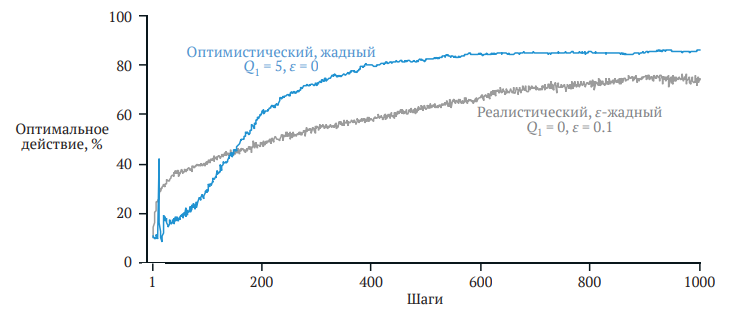
\includegraphics[width=1\linewidth]{fig_2_3.png}
    \caption{Рис. 2.3. Демонстрация оптимистических начальных оценок ценности действий на 10-руком испытательном стенде. В обоих методах размер шага постоянный, $\varepsilon$ = 0.1}
\end{figure}
\begin{solution}
    В первые шаги оптимистическая инициализация заставляет алгоритм почти детерминированно перебрать все действия, понижая их оценки. После первичного перебора оптимальное действие, имеющее более высокое истинное среднее, сохраняет более высокую оценку по сравнению с другими, что приводит к временному увеличению доли его выбора. Именно эта синхронная фаза перебора и последующее перераспределение оценок создают наблюдаемые пики и осцилляции.
\end{solution}

\subsection{Упражнение 2.7. Несмещенный постоянный размер шага(с. 62)}
В  большей части этой главы мы использовали выборочные средние для оценки ценности действий, поскольку при этом отсутствует начальное смещение, характерное для постоянного размера шага (см. анализ в формуле (2.6)). Однако выборочное среднее – не вполне удовлетворительное решение, поскольку оно может плохо работать в нестационарных задачах. Можно ли избежать смещения в  методах с  постоянным размером шага, не отказываясь от их преимуществ в нестационарных задачах?
Один из способов – использовать размер шага
\begin{equation}
\beta_n = \alpha / o_n
\tag{2.8}
\end{equation}
для обработки n-го вознаграждения за конкретное действие, где $\alpha > 0$ – обычный постоянный размер шага, а $o_n$
 – рекуррентная последовательность, начинающаяся в 0:
\begin{equation}
o_n = o_{n-1} + \alpha \cdot (1 - o_{n-1}) \quad \text{для} \quad n\ge0, \quad \text{где} \quad o_0=0
\tag{2.9}
\end{equation}
Проведите анализ, подобный формуле (2.6), и покажите, что $Q_n$
– экспоненциальное среднее, взвешенное по степени новизны, без начального смещения
\begin{solution}
    Заметим, что $o_n - \alpha = o_{n-1} \cdot (1 - \alpha)$.\\
    Согласно $(*)$ достаточно показать, что
    \[\prod_{i=1}^{n} (1-\beta_i) = 0\]
    Действительно, 
    \[\prod_{i=1}^{n} (1-\beta_i) = \prod_{i=1}^{n} \frac{o_i-\alpha}{o_i} = (1-\alpha) \cdot \prod_{i=1}^{n} \frac{o_{i-1}}{o_i} = 0,\]
    так как $\frac{o_{0}}{o_1} = 0$
\end{solution}

\subsection{Упражнение 2.8. Пики ВДГ(с. 63)}
На рис.2.4 график, соответствующий методу ВДГ, имеет отчетливый пик на 11-м шаге. Почему? Ответ будет считаться полным, если он объясняет, почему вознаграждение увеличивается на 11-м шаге и почему уменьшается на последующих шагах. Указание: если c = 1, то пик не так сильно выражен.
\begin{figure}[H]
    \centering
    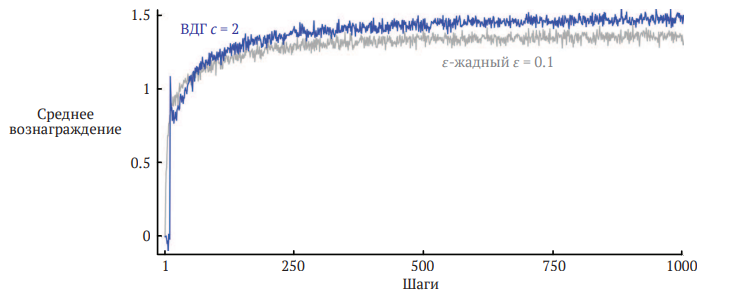
\includegraphics[width=1\linewidth]{fig_2_4.png}
    \caption{Рис. 2.4. Среднее вознаграждение за выбор ВДГ-действия на 10-руком испытательном стенде. Как видно, ВДГ, вообще говоря, работает лучше, чем $\varepsilon$-жадный выбор действия, за исключением первых $k$ шагов, когда он случайно выбирает из еще не опробованных действий}
\end{figure}
\begin{solution}
    В течение первых десяти шагов описанный алгоритм выберет по одному разу каждое из действий в случайном порядке. 11-ый шаг - это первый шаг, когда алгоритм будет выбирать действие на основании $Q(a)$. Это означает выбор действия, которое принесло наибольшую награду за первые 10 шагов.Таким образом объясняется резкое возрастание графика. После этого слагаемое
    $c \cdot \sqrt{\frac{\ln t}{N_t(a)}}$ не позволяет долго оставаться на одном действии, и алгоритм продолжает исследовать уже с учетом "недостоверности". Падение после 11-го шага объясняется постепенным уточнением ценности и последующим переключением на менее исследованные действия.
\end{solution}

\subsection{Упражнение 2.9(с. 64)}
Покажите, что в случае двух действий распределение softmax совпадает с  определяемым логистической, или сигмоидной, функцией, часто используемой в статистике и в искусственных нейронных сетях.
\begin{solution}
    Пусть у нас действия $a \in \{1, 2\}$ с логитами $H_1 \ \text{и} \ H_2$ соответственно. Тогда softmax задаёт вероятности
    \[
    \pi(1)=\frac{e^{H_1}}{e^{H_1}+e^{H_2}},
    \qquad
    \pi(2)=\frac{e^{H_2}}{e^{H_1}+e^{H_2}}.
    \]
    Преобразуем $\pi(1)$:
    \[
    \pi(1)
    = \frac{e^{H_1}}{e^{H_1}+e^{H_2}}
    = \frac{1}{1+\frac{e^{H_2}}{e^{H_1}}}
    = \frac{1}{1+e^{H_2-H_1}}
    = \frac{1}{1+e^{-(H_1-H_2)}}.
    \]
    
    Обозначим $\Delta = H_1 - H_2$. Тогда
    \[
    \pi(1)=\frac{1}{1+e^{-\Delta}}
    = \sigma(\Delta),
    \]
    где сигмоидная функция определяется как
    \[
    \sigma(x)=\frac{1}{1+e^{-x}}.
    \]
    
    Аналогично,
    \[
    \pi(2)
    = \frac{e^{H_2}}{e^{H_1}+e^{H_2}}
    = \frac{1}{1+e^{H_1-H_2}}
    = \frac{1}{1+e^{\Delta}}
    = \sigma(-\Delta)
    = 1-\sigma(\Delta).
    \]
\end{solution}

\subsection{Упражнение 2.10(с. 68)}
Пусть имеется задача о 2-руком бандите, в которой истинные ценности действий случайным образом меняются от шага к шагу. Точнее, предположим, что на любом временном шаге истинные ценности действий 1 и 2 равны соответственно 0.1 и 0.2 с вероятностью 0.5 (случай A) и 0.9 и 0.8 с вероятностью 0.5 (случай B). Если мы не можем сказать, какой случай имеет место на данном шаге, то каково максимально возможное математическое ожидание успеха и как следует себя вести, чтобы достичь его? Теперь предположим, что на каждом шагенам сообщают, какой случай, A или B, имеет место (хотя истинной ценности действий мы по-прежнему не знаем). Это задача ассоциативного поиска. Какого максимального математического ожидания успеха можно достичь в этой задаче и как следует себя вести для его достижения?
\begin{solution}
    Если игрок не знает, какой случай имеет место на данном шаге, то он использует одну и ту же стратегию вне зависимости от случая. Посчитаем средние истинные ценности:
    \[\mathbb{E}(q_*(1)) = 0.5 \cdot 0.1 + 0.5 \cdot 0.9 = 0.5\]
    \[\mathbb{E}(q_*(2)) = 0.5 \cdot 0.2 + 0.5 \cdot 0.8 = 0.5\]
    Тогда 
    \[\mathbb{E}(R_t) = \pi(1) \cdot 0.5 + (1 - \pi(1)) \cdot 0.5 = 0.5\]
    Поэтому среднее вознаграждение будет равняться 0.5 вне зависимости от политики игрока. \\
    Если же игроку известен случай на текущем шаге, то в таком случае он властен использовать разные политики в зависимости от случая. Оптимальным будет следующий выбор:
    \[\pi(1 \mid A) = 0 \quad \text{и} \quad \pi(2 \mid A) = 1\]
    \[\pi(1 \mid B) = 1 \quad \text{и} \quad \pi(2 \mid B) = 0\]
    Тогда 
    \[\mathbb{E}(R_t) = 0.5 \cdot 0.2 + 0.5 \cdot 0.9 = 0.55\]
\end{solution}

\subsection{Упражнение 2.11(с. 71)}
Создайте рисунок, аналогичный рис.2.6, только для нестационарного случая, описанного в упражнении 2.5. Включите $\varepsilon$-жадный алгоритм с постоянным размером шага и $\varepsilon = 0.1$. Количество шагов пусть будет равным 200 000, а в качестве показателя качества каждого алгоритма и значения параметра возьмите среднее вознаграждение за последние 100 000 шагов. 
\begin{figure}[H]
    \centering
    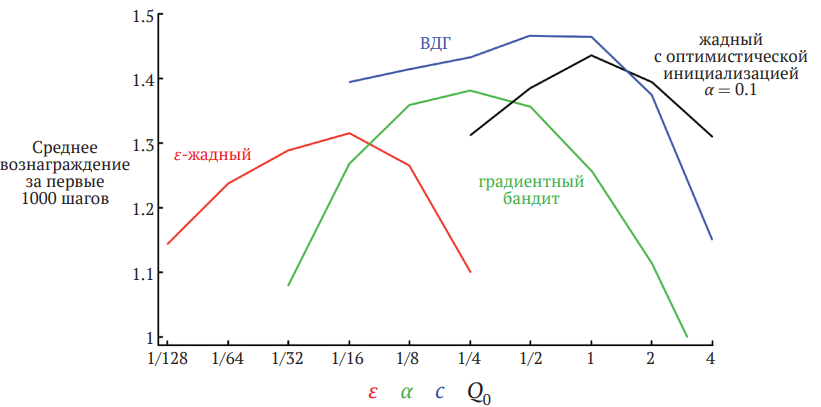
\includegraphics[width=1\linewidth]{fig_2_6.png}
    \caption{Рис. 2.6. Параметрическое исследование различных алгоритмов решения задачи о бандите, описанных в этой главе. Каждая точка – это среднее вознаграждение, полученное алгоритмом за 1000 шагов при определенном значении параметра}
\end{figure}
\begin{solution}
    \textbf{Код смотри в отдельном файле репозитория.}
    \begin{figure}[H]
        \centering
        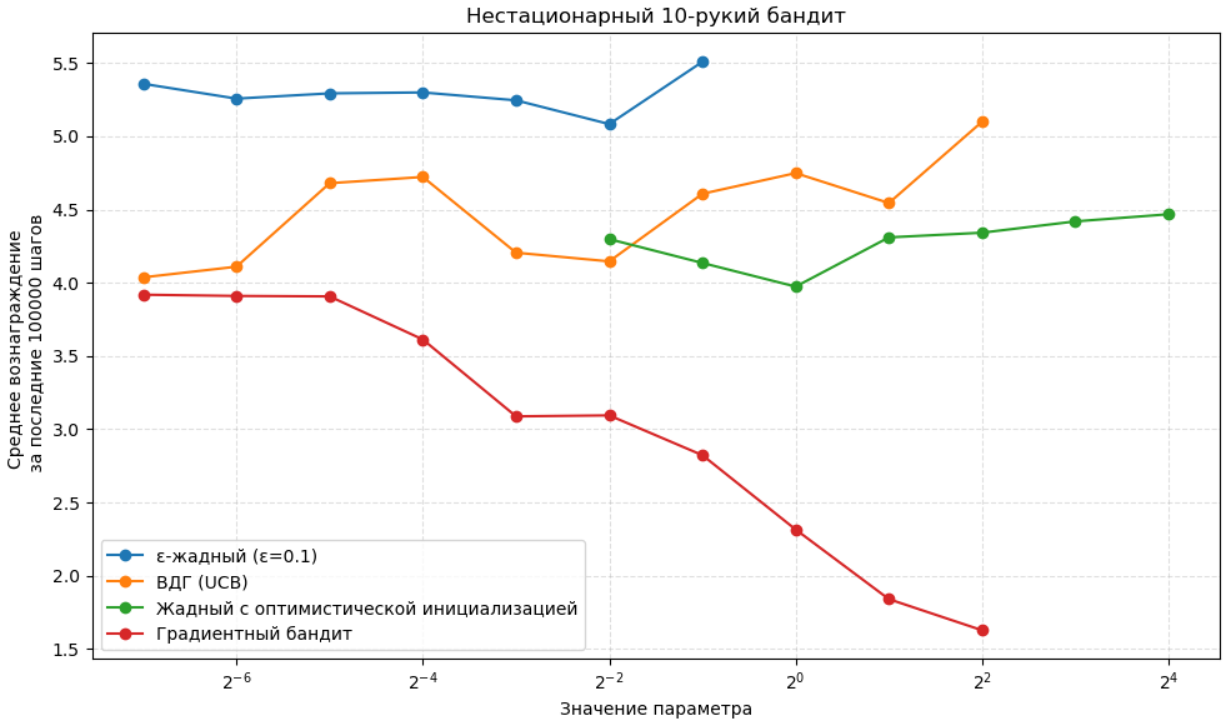
\includegraphics[width=1\linewidth]{fig_2_11_sol.png}
    \end{figure}
\end{solution}
\notebook{02_11}{2.11}

\section{Глава 3. Конечные марковские процессы принятия решений}
\subsection{Упражнение 3.1(c. 78)}
Придумайте три примера задач, укладывающихся в формализм
МППР. Определите для каждого состояния, действия и  вознаграждения. Постарайтесь, чтобы примеры как можно сильнее различались. Формализм абстрактный и гибкий, он может применяться разными способами. Хотя бы в одном примере попытайтесь подобраться к его пределам.
\begin{solution}
    \textbf{Первый пример.} Начнем с примитивного. Рассмотрим популярную в наше время задачу беспилотных автомобилей. Действиями могут быть следующие параметры: угол, на который следует повернуть руль, сила нажатия на педали тормоза/газа. Состоянием могут быть как характеристики движения, например, скорость, так и сцена возле автомобиля, полученная с лидара. Для вознаграждений же можно придумать множество реализаций. Например, это может быть сложной функцией от расстояния до ближайшего объекта. Разумно будет добавить штраф за отклонение с полосы или резкие ускорения. \\
    \textbf{Второй пример.} Выбор партнера для отношений. Поскольку у нас нет ограничений на временные шаги, то можем рассматривать тройку (состояние, действие, награда) с частотой, например, в месяц. Приведем возможные примеры действий: подарить цветы, пригласить на свидание, оплатить совместный отдых или расстаться и сменить партнера. Состояние включает в себя характеристики партнера(психические, физические), накопленные обиды, вашу удовлетворенность, ваш социальный/карьерный рост за время этих отношений. А награду введем +1000000 за заключение брачного договора, +1000 за преодоление трудностей, -1000000000000 за разбитые сердца, +100 за стабильность в отношениях. Это пример нестационарной среды, в которой распределение вероятностей зависит от текущего партнера.\\
    \textbf{Третий пример.} Рассмотрим задачу эволюции целой цивилизации как единого агента, принимающего решения раз в столетие. Действиями являются выбор научных парадигм, политических устройств, моральных норм, направлений экспансии или отказа от неё. Состояние включает суммарное знание, технологический уровень, численность населения, распределение ресурсов, устойчивость экосистемы и культурные ценности. Награда определяется выживанием цивилизации, ростом совокупного благополучия, расширением доступной Вселенной или сохранением сознательной жизни, а терминальным состоянием может быть вымирание, технологическая сингулярность или тепловая смерть локального региона космоса.
\end{solution}

\subsection{Упражнение 3.2(c. 79)}
Достаточно ли формализма МППР для полезного представления
всех задач обучения целеустремленного агента? Можете ли вы придумать очевидные исключения? 
\begin{solution}
    Во-первых, далеко не во всех задачах имеет место марковское свойство. Контрпример - покер. В этой игре $\mathbb{P}(S_{t+1}, R_{t+1} \mid S_t, A_t)$ зависит и от выбора соперника, и от прошлой истории.\\
    Во-вторых, в классической формулировке МППР подразумевается стационарность. Если среда нестационарна(те же самообучающиеся крестики-нолики из Главы $1$), то мы имеем дело с $\mathbb{P}_t(S_{t+1}, R_{t+1} \mid S_t, A_t)$. \\
    В-третьих, существует огромный круг задач, где использование награды не самым корректным образом отражает структуру задачи. Например, если рассматривать постановки, в которых человек является агентом(как в предыдущем упражнении), то его цель может не соответствовать любой предложенной награде.
\end{solution}

\subsection{Упражнение 3.3(c. 79)}
Рассмотрим задачу о  вождении автомобиля. Можно было бы
определить действия в терминах акселератора, руля и тормозов, т.е. тех мест, где ваше тело входит в контакт с машиной. А можно было бы поместить их дальше снаружи – например, там, где шина контактирует с дорогой, считая вашими действиями крутящий момент на колесе. Или поместить их дальше внутри – скажем, там, где ваш мозг вступает в контакт с телом, и считать действиями сокращения
мускулов, управляющих вашими конечностями. Или можно перейти на совсем уж высокий уровень и сказать, что ваше действие – это выбор места назначения. Какой уровень правильный, т. е. где нужно было бы провести границу между агентом и окружающей средой? На каком основании следует предпочесть одно положение границы другому? Существует ли фундаментальная причина предпочесть одно положение другому или это свободный выбор?
\begin{solution}
    Граница между агентом и средой в задаче вождения автомобиля не имеет единственного "правильного"\ положения и определяется не физикой, а целями моделирования. Предпочтение одного уровня другому носит прагматический характер: выбранная граница должна обеспечивать марковость состояния, соответствовать реально управляемым агентом переменным и приводить к разумной сложности динамики и обучения. Таким образом, фундаментальной причины предпочесть один уровень другому нет - это свободный, но осмысленный моделировочный выбор, зависящий от целей и удобства анализа.
\end{solution}

\subsection{Упражнение 3.4(c. 80)}
Постройте такую же таблицу, как в примере 3.3, но для $p(s', r \mid s, a)$. В ней должны быть столбцы $s, a, s', r$ и $p(s', r \mid s, a)$ и по одной строке для каждой четверки такой, что $p(s', r \mid s, a) > 0$.
\begin{solution}
\leavevmode\par
\medskip
    \begin{center}
    \begin{tabular}{c c c c c}
    \hline
    $s$ & $a$ & $s'$ & $r$ & $p(s',r\mid s,a)$ \\
    \hline
    high & search & high & $r_{\text{search}}$ & $\alpha$ \\
    high & search & low  & $r_{\text{search}}$ & $1-\alpha$ \\
    \hline
    high & wait   & high & $r_{\text{wait}}$   & $1$ \\
    \hline
    low  & search & low  & $r_{\text{search}}$ & $\beta$ \\
    low  & search & high & $-3$                & $1-\beta$ \\
    \hline
    low  & wait   & low  & $r_{\text{wait}}$   & $1$ \\
    \hline
    low  & recharge & high & $0$               & $1$ \\
    \hline
    \end{tabular}
    \end{center}
\end{solution}

\subsection{Упражнение 3.5(c. 83)}
Равенства в разделе $3.1$ справедливы для непрерывного случая, а для эпизодических задач их необходимо модифицировать (совсем чуть-чуть). Покажите, что вы знаете, как именно, для чего приведите модифицированный вариант формулы $(3.3)$. 
\begin{equation}
\sum_{s' \in S} \sum_{r \in R}
p(s', r \mid s, a) = 1,
\qquad
\forall\, s \in S,
\ \forall\, a \in A(s).
\tag{3.3}
\end{equation}
\begin{solution}
    \[
    \sum_{s' \in S^+} \sum_{r \in R}
    p(s', r \mid s, a) = 1,
    \qquad
    \forall\, s \in S,
    \ \forall\, a \in A(s).
    \]
\end{solution}

\subsection{Упражнение 3.6(c. 84)}
Предположим, что балансирование стержня рассматривается как эпизодическая задача, но с  использованием обесценивания, так что все вознаграждения равны $0$, кроме вознаграждения за неудачу, равного $-1$. Каким тогда будет доход в каждый момент времени? Чем этот доход отличается от дохода в непрерывной задаче с обесцениванием?
\begin{solution}
    В такой постановке задачи доход также будет определяться величиной $-\gamma^K$, где $K$ - количество временных шагов до наступления неудачи. В случае эпизодической задачи 
    \[G_t = -\gamma^K\]
    После неудачи эпизод заканчивается и начинается следующий. В непрерывной же задаче переключения эпизода не происходит и доход выглядит следующим образом:
    \[G_t = -\gamma^{K_1} - \gamma^{K_2} - \dots - \gamma^{K_n} - \dots,\]
    где $K_i$ - момент неудачи в $i$-ой попытке.
\end{solution}

\subsection{Упражнение 3.7(c. 84)}
Допустим, вы проектируете робота для прохождения лабиринта. Вы решили давать вознаграждение $+1$ за выход из лабиринта и $0$ в остальных случаях. Похоже, задача естественно распадается на эпизоды – последовательные прохождения лабиринта, поэтому вы решили рассматривать ее как эпизодическую, в которой цель – максимизировать ожидаемое полное вознаграждение $(3.7)$. Погоняв некоторое время обучающегося агента, вы обнаружили полное отсутствие прогресса. Что не так? Достаточно ли доходчиво вы сообщили агенту, чего именно он должен достичь?
\begin{solution}
    Запишем формулу дохода для случайного эпизода:
    \[G_t = r_{t+1} + r_{t+2} + \dots + r_T\]
    Вышеупомянутое определение вознаграждения вне зависимости от длины эпизода $T$ приводит к тому, что
    \[r_{t+1} = r_{t+2} = \dots = r_{T-1} = 0 \quad \text{и} \quad r_T = 1\]
    Тогда в любом эпизоде $G_t = 1$. Из этого следует, что награда никак не согласуется со временем, потраченным на поиск выхода из лабиринта. С точки зрения вознаграждения эпизод, когда робот долго не мог найти выход и блуждал по лабиринту, будет равен эпизоду, когда робот нашел выход за минимальное число шагов. Решением будет, например, добавить дисконтирование($\gamma$).
\end{solution}

\subsection{Упражнение 3.8(c. 84)}
Предположим, что $\gamma = 0.5$, последовательность полученных вознаграждений имеет вид: $R_1 = -1, R_2 = 2, R_3 = 6, R_4 = 3, R_5 = 2 \ \text{и} \ T = 5$. Чему равны $G_0, G_1, \dots , G_5$? Указание: идите от конца к началу.
\begin{solution}
    Используем рекурсивное определение дохода:
    \[
    G_t = R_{t+1} + \gamma G_{t+1}, 
    \qquad G_T = 0.
    \]
    
    Дано: 
    \[
    \gamma = 0.5, \quad 
    R_1=-1,\; R_2=2,\; R_3=6,\; R_4=3,\; R_5=2, \quad T=5.
    \]
    
    Вычисляем с конца.
    
    \[
    G_5 = 0.
    \]
    
    \[
    G_4 = R_5 + \gamma G_5
         = 2 + 0.5 \cdot 0
         = 2.
    \]
    
    \[
    G_3 = R_4 + \gamma G_4
         = 3 + 0.5 \cdot 2
         = 3 + 1
         = 4.
    \]
    
    \[
    G_2 = R_3 + \gamma G_3
         = 6 + 0.5 \cdot 4
         = 6 + 2
         = 8.
    \]
    
    \[
    G_1 = R_2 + \gamma G_2
         = 2 + 0.5 \cdot 8
         = 2 + 4
         = 6.
    \]
    
    \[
    G_0 = R_1 + \gamma G_1
         = -1 + 0.5 \cdot 6
         = -1 + 3
         = 2.
    \]
    
    Итак,
    \[
    G_0 = 2, \quad
    G_1 = 6, \quad
    G_2 = 8, \quad
    G_3 = 4, \quad
    G_4 = 2, \quad
    G_5 = 0.
    \]
\end{solution}

\subsection{Упражнение 3.9(c. 84)}
Предположим, что $\gamma = 0.9$ и последовательность вознаграждений начинается с $R_1 = 2$, за которым следует бесконечная последовательность чисел $7$.
Чему равны $G_0$ и $G_1$? 
\begin{solution}
    По определению дохода:
    \[
    G_t = \sum_{k=0}^{\infty} \gamma^k R_{t+k+1}.
    \]
    Тогда
    \[
    G_1 = 7 + 0.9 \cdot 7 + 0.9^2 \cdot 7 + \dots = 
    7 \cdot \sum_{k=0}^{\infty} (0.9)^k
     = 7 \cdot \frac{1}{1-0.9}
     = 7 \cdot \frac{1}{0.1}
     = 70.
    \]
    Пользуясь рекурсивной формулой,
    \[G_0 = R_1 + \gamma \cdot G_1 
     = 2 + 0.9 \cdot 70
     = 2 + 63
     = 65.\]
\end{solution}

\subsection{Упражнение 3.10(c. 84)}
Докажите равенство $(3.10)$.
\begin{equation}
G_t = \sum_{k=0}^{\infty} \gamma^k = \frac{1}{1 - \gamma}, \qquad 0 < \gamma < 1
\tag{3.10}
\end{equation}
\begin{solution}
    Рассмотрим частичную сумму геометрического ряда:
    \[
    S_n=\sum_{k=0}^{n}\gamma^k.
    \]
    Из формулы суммы геометрической прогрессии:
    \[
    S_n=\frac{1-\gamma^{\,n+1}}{1-\gamma}.
    \]
    Так как $\gamma<1$, то $\gamma^{\,n+1}\to 0$ при $n\to\infty$. Следовательно,
    \[
    \sum_{k=0}^{\infty}\gamma^k
    =\lim_{n\to\infty} S_n
    =\lim_{n\to\infty}\frac{1-\gamma^{\,n+1}}{1-\gamma}
    =\frac{1}{1-\gamma}.
    \]
\end{solution}

\subsection{Упражнение 3.11(c. 86)}
Если текущее состояние равно $S_t$ и действия выбираются согласно стохастической стратегии $\pi$, то каково математическое ожидание $R_{t+1}$
в терминах $\pi$ и функции $p$ с четырьмя аргументами (3.2)?
\begin{equation}
p(s', r \mid s, a)
=
\mathbb{P}\!\bigl\{ S_t = s',\, R_t = r \,\big|\, S_{t-1} = s,\, A_{t-1} = a \bigr\}.
\tag{3.2}
\end{equation}
\begin{solution}
    \[
    \begin{aligned}
    \mathbb{E}\!\left[R_{t+1}\mid S_t=s\right]
    &= \sum_{r\in R} r\,\mathbb{P}\!\left(R_{t+1}=r\mid S_t=s\right) \\
    &= \sum_{r\in R} r \sum_{a\in A(s)} \pi(a\mid s)
    \sum_{s'\in S} p(s',r \mid s,a).
    \end{aligned}
    \]
\end{solution}

\subsection{Упражнение 3.12(c. 86)}
Выразите $v_\pi$ через $q_\pi$ и $\pi$.
\[
    v_{\pi}(s)
    =
    \mathbb{E}_{\pi}\!\left[ G_t \mid S_t = s \right]
    =
    \mathbb{E}_{\pi}\!\left[ \left. \sum_{k=0}^{\infty} \gamma^k R_{t+k+1} \,\right|\, S_t = s \right],
    \quad \text{для всех } s \in S.
\]
\[
    q_{\pi}(s,a)
    =
    \mathbb{E}_{\pi}\!\left[ G_t \mid S_t = s, A_t = a \right]
    =
    \mathbb{E}_{\pi}\!\left[ \left. \sum_{k=0}^{\infty} \gamma^k R_{t+k+1}
    \,\right|\, S_t = s, A_t = a \right].
\]
\begin{solution}
    \begin{align*}
    v_\pi(s)
    &= \mathbb{E}_\pi\!\left[ G_t \mid S_t = s \right] =\\
    &= \sum_{a\in A(s)} \mathbb{P}_\pi(A_t=a \mid S_t=s)\,
       \mathbb{E}_\pi\!\left[ G_t \mid S_t=s, A_t=a \right] =\\
    &= \sum_{a\in A(s)} \pi(a\mid s)\, q_\pi(s,a).
    \end{align*}
\end{solution}

\subsection{Упражнение 3.13(c. 86)}
Выразите $q_\pi$ через $v_\pi$ и функцию $p$ с четырьмя аргументами. .
\[
    v_{\pi}(s)
    =
    \mathbb{E}_{\pi}\!\left[ G_t \mid S_t = s \right]
    =
    \mathbb{E}_{\pi}\!\left[ \left. \sum_{k=0}^{\infty} \gamma^k R_{t+k+1} \,\right|\, S_t = s \right],
    \quad \text{для всех } s \in S.
\]
\[
    q_{\pi}(s,a)
    =
    \mathbb{E}_{\pi}\!\left[ G_t \mid S_t = s, A_t = a \right]
    =
    \mathbb{E}_{\pi}\!\left[ \left. \sum_{k=0}^{\infty} \gamma^k R_{t+k+1}
    \,\right|\, S_t = s, A_t = a \right].
\]
\[
p(s', r \mid s, a)
=
\mathbb{P}\!\bigl\{ S_t = s',\, R_t = r \,\big|\, S_{t-1} = s,\, A_{t-1} = a \bigr\}.
\]
\begin{solution}
    \[
    q_\pi(s,a)
    = \mathbb{E}_\pi\!\left[ G_t \mid S_t=s, A_t=a \right]
    = \sum_{s'\in S}\sum_{r\in R} p(s',r\mid s,a)\,\Bigl(r + \gamma\, v_\pi(s')\Bigr).
    \]
\end{solution}

\subsection{Упражнение 3.14(c. 89)}
Уравнение Беллмана $(3.14)$ должно выполняться в  каждом состоянии для функции ценности $v_{\pi}$, показанной на рис. $3.2$ (справа) в примере  $3.5$. Покажите численно, что это уравнение выполняется для центрального состояния с ценностью $+0.7$ по отношению к четырем его соседним состояниям
с ценностями $+2.3$, $+0.4$, $-0.4$ и $+0.7$. (Точность этих чисел – всего один знак после запятой.)
\begin{equation}
    v_\pi(s)
    =
    \sum_{a} \pi(a \mid s)
    \sum_{s',r} p(s', r \mid s, a)
    \bigl[ r + \gamma v_\pi(s') \bigr]
\tag{3.14}
\end{equation}
\begin{solution}
    Для примера 3.5 стратегия равновероятная, поэтому
    \[
    \pi(a\mid s)=\frac14,\qquad a\in\{\text{север, юг, запад, восток}\},
    \]
    а для центрального состояния все переходы детерминированы в соседние клетки и дают награду \(r=0\).
    Также в примере используется \(\gamma=0.9\).
    
    Тогда уравнение Беллмана (3.14) для этого состояния принимает вид
    \[
    v_\pi(s)=\frac14 \sum_{a}\bigl[0+\gamma v_\pi(s_a)\bigr]
    =\frac{\gamma}{4}\Bigl(v_\pi(s_{\uparrow})+v_\pi(s_{\downarrow})+v_\pi(s_{\leftarrow})+v_\pi(s_{\rightarrow})\Bigr).
    \]
    
    Подставим значения соседей \(2.3,\;0.4,\;-0.4,\;0.7\):
    \[
    v_\pi(s)=\frac{0.9}{4}\,(2.3+0.4-0.4+0.7)
    =\frac{0.9}{4}\cdot 3.0
    =0.675 \approx 0.7.
    \]
    
    Получили \(v_\pi(s)\approx 0.7\), что согласуется с указанной на рисунке величиной (с точностью до одного знака после запятой).
\end{solution}

\subsection{Упражнение 3.15(c. 89)}
В примере сеточного мира вознаграждения положительны для
целей, отрицательны для выхода на края мира и равны нулю в остальных случаях. Что важно: знаки вознаграждений или только расстояния между ними? Докажите, пользуясь формулой $(3.8)$, что прибавление константы c ко всем вознаграждениям прибавляет константу $v_c$ к ценностям всех состояний и потому не влияет на относительные ценности состояний при любой стратегии. Выразите $v_c$
 через $c$ и $\gamma$.
\begin{equation}
    G_t = R_{t+1} + \gamma R_{t+2} + \gamma^2 R_{t+3} + \cdots
= \sum_{k=0}^{\infty} \gamma^k R_{t+k+1}.
\tag{3.8}
\end{equation}
\begin{solution}
    Рассмотрим
    \[
    R'_{t+k+1}=R_{t+k+1}+c,\qquad k=0,1,2,\dots
    \]
    Тогда по формуле (3.8) новый доход
    \[
    \begin{aligned}
    G'_t
    &= \sum_{k=0}^{\infty}\gamma^k R'_{t+k+1}
    = \sum_{k=0}^{\infty}\gamma^k (R_{t+k+1}+c) \\
    &= \sum_{k=0}^{\infty}\gamma^k R_{t+k+1}
    + c\sum_{k=0}^{\infty}\gamma^k
    = G_t + c\sum_{k=0}^{\infty}\gamma^k.
    \end{aligned}
    \]
    При $0 < \gamma<1$ имеем геометрическую сумму
    \[
    \sum_{k=0}^{\infty}\gamma^k=\frac{1}{1-\gamma},
    \]
    поэтому
    \[
    G'_t=G_t+\frac{c}{1-\gamma}.
    \]
    Обозначим ценность состояния:
    \[
    v_\pi(s)=\mathbb{E}_\pi[G_t\mid S_t=s],\qquad
    v'_\pi(s)=\mathbb{E}_\pi[G'_t\mid S_t=s].
    \]
    Берем математическое ожидание:
    \[
    v'_\pi(s)=\mathbb{E}_\pi\!\left[G_t+\frac{c}{1-\gamma}\,\middle|\,S_t=s\right]
    =\mathbb{E}_\pi[G_t\mid S_t=s]+\frac{c}{1-\gamma}
    =v_\pi(s)+v_c,
    \]
    где
    \[
    v_c=\frac{c}{1-\gamma}.
    \]
    Следовательно, для любых $s_1,s_2$:
    \[
    v'_\pi(s_1)-v'_\pi(s_2)=(v_\pi(s_1)+v_c)-(v_\pi(s_2)+v_c)=v_\pi(s_1)-v_\pi(s_2),
    \]
    то есть прибавление константы $c$ ко всем вознаграждениям сдвигает значения всех состояний на одну и ту же константу $v_c$
    и не влияет на их относительные ценности при любой стратегии $\pi$.
\end{solution}

\subsection{Упражнение 3.16(c. 89)}
Теперь рассмотрим прибавление константы $c$ ко всем вознаграждениям в эпизодической задаче, например о прохождении лабиринта. Будет ли это иметь какой-то эффект или задача останется такой же, как в случае непрерывной задачи выше? Почему? Приведите пример. 
\begin{solution}
Рассмотрим обесцененную версию эпизодической задачи. Пусть эпизод завершается за случайное число шагов $T$.
Исходный доход:
\[
G_t=\sum_{k=0}^{T-t-1}\gamma^k R_{t+k+1}.
\]
После сдвига вознаграждений $R'_{t+k+1}=R_{t+k+1}+c$ получаем
\[
G'_t
=\sum_{k=0}^{T-t-1}\gamma^k (R_{t+k+1}+c)
=G_t + c\sum_{k=0}^{T-t-1}\gamma^k.
\]
Геометрическая сумма теперь зависит от длины эпизода:
\[
\sum_{k=0}^{T-t-1}\gamma^k
=\frac{1-\gamma^{T-t}}{1-\gamma}.
\]
Следовательно,
\[
G'_t
=G_t + \frac{c(1-\gamma^{T-t})}{1-\gamma}.
\]
В отличие от непрерывной задачи, добавка зависит от $T-t$,
то есть от того, сколько шагов осталось до завершения.
Поэтому разные траектории получают разные добавки,
и относительные ценности состояний меняются.

\textbf{Пример.}
Рассмотрим задачу лабиринта с $\gamma=1$, нулевыми наградами на каждом шагеи $+1$ в терминальном состоянии.
Тогда $G_t=1$ независимо от длины пути.

Теперь прибавим $c=1$ ко всем наградам. Тогда каждый шаг даёт $+1$, а в конце ещё $+1$.
Доход равен:
\[
G'_t = T-t+1.
\]
Теперь выгодно затягивать эпизод как можно дольше.
Оптимальная стратегия изменилась.

Следовательно, в эпизодических задачах прибавление константы ко всем вознаграждениям меняет задачу, поскольку дополнительная сумма зависит от длины эпизода.
\end{solution}

\subsection{Упражнение 3.17(c. 90)}
\begin{wrapfigure}{r}{0.3\textwidth}
    \centering
    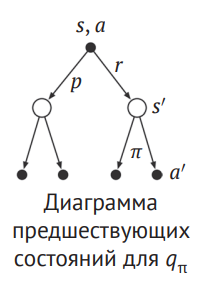
\includegraphics[width=0.25\textwidth]{q_pi_graph.png}
\end{wrapfigure}
Как выглядит уравнение Беллмана для ценностей действий, т. е. для $q_{\pi}$? Оно должно выражать ценность действия $q_{\pi}(s, a)$ в терминах ценностей действий $q_{\pi}(s', a')$ возможных преемников пары состояние–действие $(s, a)$. Указание: этому уравнению соответствует диаграмма предшествующих состояний справа. Выпишите последовательность равенств, аналогичную $(3.14)$, но для ценностей действий.
\begin{solution}
    Воспользуемся результатом упражнений 3.12 и 3.13:
    \begin{align*}
    q_\pi(s,a)
    &= \mathbb{E}_\pi\!\left[ G_t \mid S_t=s, A_t=a \right] = \\
    &= \sum_{s'\in S}\sum_{r\in R} p(s',r\mid s,a)\,\Bigl(r + \gamma\, v_\pi(s')\Bigr)  = \\
    &= \sum_{s'\in S}\sum_{r\in R} p(s',r\mid s,a)\,\Bigl(r + \gamma\sum_{a'\in A(s')} \pi(a'\mid s')\, q_\pi(s',a')\Bigr) 
    \end{align*}
\end{solution}

\subsection{Упражнение 3.18(c. 90)}
Ценность состояния зависит от ценностей действий, возможных в этом состоянии, и от вероятностей выбора
действий при текущей стратегии. Мы можем представить это в виде небольшой диаграммы предшествующих состояний с корнем в состоянии, на которой показаны все возможные действия:
\begin{figure}[H]
    \centering
    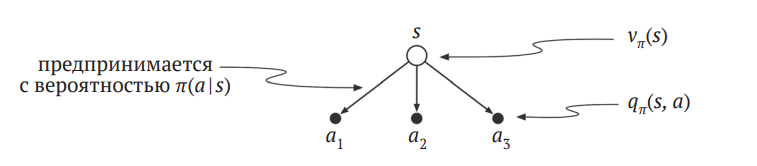
\includegraphics[width=0.8\linewidth]{fig_3_18_task.png}
\end{figure}
Выпишите уравнение, соответствующее этому интуитивному представлению и диаграмме для ценности в корневом узле $v_{\pi}(s)$, в терминах ценности в ожидаемом
листовом узле $q_{\pi}(s, a)$, при условии что $S_t = s$. Это уравнение должно включать математическое ожидание, обусловленное следованием стратегии $\pi$. Затем выпишите
второе уравнение, в котором ожидаемая ценность выражена явно через $\pi(a | s)$, так чтобы никакого математического ожидания ценности в уравнение не входило. 
\begin{solution}
\[
v_\pi(s)=\mathbb{E}_\pi\!\left[q_\pi(s,A_t)\mid S_t=s\right].
\]
Если множество действий дискретно, то это ожидание можно выписать явно через вероятности выбора действий:
\[
v_\pi(s)=\sum_{a}\pi(a\mid s)\,q_\pi(s,a).
\]
\end{solution}

\subsection{Упражнение 3.19(c. 91)}
Ценность действия $q_{\pi}(s, a)$ зависит от следующего ожидаемого вознаграждения и математического ожидания суммы оставшихся вознаграждений. И снова мы можем рассуждать о задаче, опираясь на небольшую диаграмму предшествующих состояний, на этот раз с корнем в действии (паре 
состояние-действие), которое ведет в одно из следующих возможных состояний:
\begin{figure}[H]
    \centering
    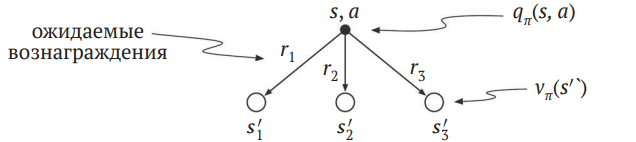
\includegraphics[width=0.7\linewidth]{fig_3_19_task.png}
\end{figure}
Выпишите уравнение, соответствующее этому интуитивному представлениюи диаграмме для ценности действия 
$q_{\pi}(s, a)$, в терминах следующего ожидаемого
вознаграждения $R_{t+1}$ и ожидаемой ценности следующего состояния $v_{\pi}(S_{t+1})$, при условии что $S_t = s$ и $A_t = a$. Это уравнение должно включать математическое
ожидание, но \emph{не} обусловленное следованием стратегии. Затем выпишите второе уравнение, в  котором ожидаемая ценность выражена явно через величину $p(s', r \mid s, a)$, определенную в $(3.2)$, так чтобы никакого математического ожидания ценности в уравнение не входило.
\begin{equation}
p(s', r \mid s, a)
=
\mathbb{P}\!\bigl\{ S_t = s',\, R_t = r \,\big|\, S_{t-1} = s,\, A_{t-1} = a \bigr\}.
\tag{3.2}
\end{equation}
\begin{solution}
При фиксированных $S_t=s$ и $A_t=a$ случайность обусловлена только динамикой среды, поэтому
\[
q_\pi(s,a)=\mathbb{E}\!\left[\,R_{t+1}+\gamma\,v_\pi(S_{t+1}) \,\middle|\, S_t=s,\ A_t=a\right].
\]
Расписывая это ожидание явно через модель среды $p(s',r\mid s,a)$ из (3.2), получаем
\[
q_\pi(s,a)=\sum_{s'}\sum_{r} p(s',r\mid s,a)\,\Bigl(r+\gamma\,v_\pi(s')\Bigr).
\]
\end{solution}

\subsection{Упражнение 3.20(c. 96)}
Нарисуйте или опишите оптимальную функцию ценности состояний для примера игры в гольф. 
\begin{solution}
    В примере 3.7 описана оптимальная стратегия: два удара драйвером и один паттером. Оптимальная функция ценности состояний соответствует именно этой политике. Поэтому 
    \[
    v_*(s) =
    \begin{cases}
    -1, & \text{в области грина}, \\
    -2, & \text{где $q_*(s, \text{driver})=-2$}, \\
    -3, & \text{где $q_*(s, \text{driver})=-3$}, \\
    \dots
    \end{cases}
    \]
\end{solution}

\subsection{Упражнение 3.21(c. 96)}
Нарисуйте или опишите линии уровня оптимальной функции
ценности действий для игры паттером, $q_*(s,\text{putter})$, в примере игры в гольф.
\begin{solution}
    Не ограничивая общности, предположим, что линии уровня $-2, -3$ функции $q_*(s, \text{driver})$ совпадают  с линиями уровня $-3, -6$ функции $q_*(s, \text{putter})$ соответственно. \\
    Выбор действия согласно $q_*(s,\text{putter})$ означает, что из состояния $s$ первый шаг мы делаем паттером, а дальше действуем оптимальным образом. \\
    Поэтому 
    \[
    q_*(s,\text{putter}) =
    \begin{cases}
    -1, & \text{в области грина}, \\
    -2, & \text{где $v_{\text{putt}}(s)=-2$}, \\
    -3, & \text{где $-4 \le v_{\text{putt}}(s) \le -3$}, \\
    -4, & \text{где $-7 \le v_{\text{putt}}(s) \le -5$}, \\
    \dots
    \end{cases}
    \]
\end{solution}

\subsection{Упражнение 3.22(c. 96)}
\begin{wrapfigure}{r}{0.3\textwidth}
    \centering
    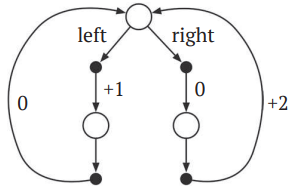
\includegraphics[width=0.25\textwidth]{fig_3_22_task.png}
\end{wrapfigure}
Рассмотрим непрерывный МППР, показанный на рисунке справа. Единственное решение принимается в верхнем состоянии, в котором возможно два действия, $left$ и $right$. Числа обозначают детерминированные вознаграждения за каждое действие. Имеется ровно две детерминированные стратегии, $\pi_{left}$ и $\pi_{right}$. Какая стратегия оптимальна, если $\gamma = 0$? А если $\gamma = 0.9$? А если $\gamma = 0.5$?
\begin{solution}
    Решение принимается только в состоянии $s_0$. После выбора действия процесс детерминированно возвращается в $s_0$ за два шага.

    \textbf{Стратегия $\pi_{left}$.}
    
    Последовательность наград:
    \[
    (+1,\,0,\,+1,\,0,\,+1,\,0,\dots)
    \]
    
    Тогда
    \[
    v_{left}(s_0)
    =
    1 + \gamma^2 + \gamma^4 + \dots
    =
    \frac{1}{1-\gamma^2}.
    \]
    
    \textbf{Стратегия $\pi_{right}$.}
    
    Последовательность наград:
    \[
    (0,\,+2,\,0,\,+2,\,0,\,+2,\dots)
    \]
    
    Тогда
    \[
    v_{right}(s_0)
    =
    2\gamma + 2\gamma^3 + 2\gamma^5 + \dots
    =
    \frac{2\gamma}{1-\gamma^2}.
    \]
    
    \textbf{Подсчёт для заданных значений $\gamma$:}
    
    \[
    \gamma = 0:
    \quad
    v_{left} = 1,
    \quad
    v_{right} = 0.
    \]
    
    \[
    \gamma = 0.9:
    \quad
    v_{left} = \frac{1}{1-0.81} = \frac{1}{0.19} \approx 5.26,
    \quad
    v_{right} = \frac{1.8}{0.19} \approx 9.47.
    \]
    
    \[
    \gamma = 0.5:
    \quad
    v_{left} = \frac{1}{1-0.25} = \frac{1}{0.75} = \frac{4}{3},
    \quad
    v_{right} = \frac{1}{0.75} = \frac{4}{3}.
    \]
\end{solution}

\subsection{Упражнение 3.23(c. 96)}
Выпишите уравнение Беллмана для $q_*$ в задаче о роботе-уборщике.
\begin{solution}
    Уравнение оптимальности Беллмана:
    \[
    q_*(s,a)=\sum_{s', r} p(s',r\mid s,a)\Bigl[r(s,a,s')+\gamma \max_{a'} q_*(s',a')\Bigr].
    \]
    
    Для робота-уборщика:
    \[
    q_*(h,s)
    =\alpha\Bigl[r_s+\gamma \max_{a'} q_*(h,a')\Bigr]
    +(1-\alpha)\Bigl[r_s+\gamma \max_{a'} q_*(l,a')\Bigr].
    \]
    
    \[
    q_*(h,w)
    =r_w+\gamma \max_{a'} q_*(h,a').
    \]
    
    \[
    q_*(l,s)
    =\beta\Bigl[r_s+\gamma \max_{a'} q_*(l,a')\Bigr]
    +(1-\beta)\Bigl[-3+\gamma \max_{a'} q_*(h,a')\Bigr].
    \]
    
    \[
    q_*(l,w)
    =r_w+\gamma \max_{a'} q_*(l,a').
    \]
    
    \[
    q_*(l,r)
    =\gamma \max_{a'} q_*(h,a').
    \]
\end{solution}

\subsection{Упражнение 3.24(c. 96)}
Рисунок $3.5$ показывает, что оптимальная ценность лучшего состояния сеточного мира равна $24.4$ с точностью до одного знака после запятой. Воспользуйтесь своим знанием оптимальной стратегии и формулой $(3.8)$, чтобы выразить эту ценность символически, а затем вычислите ее с тремя знаками после запятой. 
\begin{figure}[H]
    \centering
    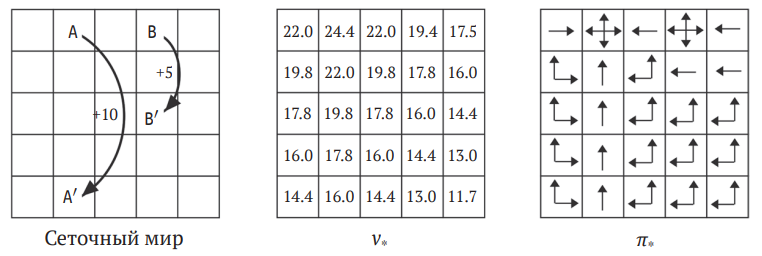
\includegraphics[width=0.75\linewidth]{fig_3_5.png}
    \caption{Рис. 3.5. Оптимальные решения задачи о сеточном мире}
\end{figure}
\begin{equation}
    G_t = R_{t+1} + \gamma R_{t+2} + \gamma^2 R_{t+3} + \cdots
= \sum_{k=0}^{\infty} \gamma^k R_{t+k+1}.
\tag{3.8}
\end{equation}
\begin{solution}
    Наилучшее состояние - $A$. Согласно оптимальной стратегии, из $A$
    агент получает вознаграждение $+10$ и мгновенно переходит в $A'$.
    Далее за $4$ шага с нулевыми наградами он возвращается в $A$,
    после чего цикл повторяется.
    
    Следовательно, начиная из $A$, ненулевые награды возникают
    через каждые $5$ шагов:
    \[
    10,\;\gamma^{5} \cdot 10,\;\gamma^{10}\cdot  10,\;\ldots
    \]
    
    По формуле (3.8)
    \[
    v_*(A)
    =
    \sum_{k=0}^{\infty} \gamma^k R_{t+k+1}
    =
    10 + \gamma^{5} \cdot 10 + \gamma^{10} \cdot 10 + \cdots
    =
    \frac{10}{1-\gamma^{5}}.
    \]
    
    При $\gamma = 0.9$ получаем
    \[
    v_*(A)
    =
    \frac{10}{1-0.9^{5}}
    =
    24.419.
    \]
\end{solution}

\subsection{Упражнение 3.25(c. 96)}
Запишите уравнение для $v_*$ в терминах $q_*$. 
\begin{solution}
    \[
    v_*(s)=\max_{a \in A(s)} q_*(s,a), \quad \forall s\in S.
    \]
\end{solution}

\subsection{Упражнение 3.26(c. 96)}
Запишите уравнение для $q_*$ в терминах $v_*$ и функции $p$ с четырьмя аргументами. 
\begin{solution}
    \[
    q_*(s,a)
    =
    \sum_{s',r}
    p(s',r \mid s,a)
    \left[
    r + \gamma v_*(s')
    \right],
    \quad \forall s \in S,\; a \in A(s).
    \]
\end{solution}

\subsection{Упражнение 3.27(c. 96)}
Запишите уравнение для $\pi_*$ в терминах $q_*$. 
\begin{solution}
    \[
    \pi_*(a\mid s)=
    \begin{cases}
    1, & a = \arg\max\limits_{a'} q_*(s,a'),\\[4pt]
    0, & \text{иначе},
    \end{cases}
    \qquad \forall s\in S,\; a\in A(s).
    \]
\end{solution}

\subsection{Упражнение 3.28(c. 96)}
Запишите уравнение для $\pi_*$ в терминах $v_*$ и функции $p$ с четырьмя аргументами.
\begin{solution}
    \[
    \begin{aligned}
    \pi_*(a \mid s)=
    &\begin{cases}
    1, 
    & a = \displaystyle
    \arg\max_{a'} \sum_{s',r} p(s',r \mid s,a')
    \bigl[ r + \gamma v_*(s') \bigr],
    \\[10pt]
    0,
    & \text{иначе},
    \end{cases} \\
    &\forall s \in S,\; a \in A(s).
    \end{aligned}
    \]
\end{solution}

\subsection{Упражнение 3.29(c. 96)}
Перепишите все четыре уравнения Беллмана для четырех функций ценности $(v_{\pi}, v_*, q_{\pi}, q_*)$ в  терминах функции $p$ с  тремя аргументами (3.4) и функции $r$ с двумя аргументами (3.5).
\begin{equation}
p(s' \mid s,a)
=
\Pr\{ S_t = s' \mid S_{t-1} = s,\; A_{t-1} = a \}
=
\sum_{r \in R} p(s',r \mid s,a).
\tag{3.4}
\end{equation}
\begin{equation}
r(s,a)
=
\mathbb{E}\!\left[ R_t \mid S_{t-1}=s,\; A_{t-1}=a \right]
=
\sum_{r \in R} r 
\sum_{s' \in S} 
p(s',r \mid s,a).
\tag{3.5}
\end{equation}
\begin{solution}
    \textbf{1. Уравнение Беллмана для $v_{\pi}$:}
    \[
    v_{\pi}(s)
    =
    \sum_{a} \pi(a \mid s)
    \left[
    r(s,a)
    +
    \gamma
    \sum_{s'} p(s' \mid s,a)\, v_{\pi}(s')
    \right].
    \]
    
    \textbf{2. Уравнение оптимальности для $v_*$:}
    \[
    v_{*}(s)
    =
    \max_{a}
    \left[
    r(s,a)
    +
    \gamma
    \sum_{s'} p(s' \mid s,a)\, v_{*}(s')
    \right].
    \]
    
    \textbf{3. Уравнение Беллмана для $q_{\pi}$:}
    \[
    q_{\pi}(s,a)
    =
    r(s,a)
    +
    \gamma
    \sum_{s'} p(s' \mid s,a)
    \sum_{a'} \pi(a' \mid s')\, q_{\pi}(s',a').
    \]
    
    \textbf{4. Уравнение оптимальности для $q_*$:}
    \[
    q_{*}(s,a)
    =
    r(s,a)
    +
    \gamma
    \sum_{s'} p(s' \mid s,a)
    \max_{a'} q_{*}(s',a').
    \]
\end{solution}

\section{Глава 4. Динамическое программирование}
\subsection{Упражнение 4.1(c. 105)}
В примере 4.1, если $\pi$ – равновероятная случайная стратегия, чему равно $q_{\pi}(11, \text{down})$? А чему равно $q_{\pi}(7, \text{down})$?
\begin{solution}
    \[
    q_{\pi}(s,a)=\sum_{s',r} p(s',r\mid s,a)\,\bigl[r+\gamma v_{\pi}(s')\bigr]
    \]
    Из постановки задачи 
    \[\gamma=1,\quad r=-1\ \text{на всех переходах},\quad v_{\pi}(T)=0.\]
    \[
    q_{\pi}(11,\text{down})
    =1\cdot\,[-1+v_{\pi}(T)]=-1 + 0 = -1.
    \]
    
    \[
    q_{\pi}(7,\text{down})
    =1\cdot\,[-1+v_{\pi}(11)]
    =-1-14=-15.
    \]
\end{solution}

\subsection{Упражнение 4.2(c. 106)}
В примере $4.1$ предположим, что добавлено новое состояние $15$ под состоянием $13$, а действия left, up, right, down в нем переводят агента в состояния $12, 13, 14$ и $15$ соответственно. Переходы из старых состояний не изменились.
Чему тогда равно $v_{\pi}(15)$ при следовании равновероятной случайной стратегии? Теперь предположим, что динамика состояния $13$ тоже изменилась, так что действие down переводит агента в новое состояние $15$. Чему в этом случае равно $v_{\pi}(15)$ при следовании равновероятной случайной стратегии? 
\begin{solution}
    Уравнение Беллмана:
    \[
    v_{\pi}(s)=\sum_a \pi(a\mid s)
    \sum_{s'} p(s'\mid s,a)\,[ -1 + v_{\pi}(s') ]
    \]
    
    Рассмотрим \textbf{случай без изменения переходов}. Тогда
    \[
    v_{\pi}(15)
    =\frac14\Big[
    (-1+v_{\pi}(12))
    +(-1+v_{\pi}(13))
    +(-1+v_{\pi}(14))
    +(-1+v_{\pi}(15))
    \Big].
    \]
    
    Отсюда
    \[
    4v_{\pi}(15)
    =
    -4+v_{\pi}(12)+v_{\pi}(13)+v_{\pi}(14)+v_{\pi}(15),
    \]
    \[
    3v_{\pi}(15)
    =
    -4+v_{\pi}(12)+v_{\pi}(13)+v_{\pi}(14).
    \]
    
    Из примера 4.1:
    \[
    v_{\pi}(12)=-22,\qquad
    v_{\pi}(13)=-20,\qquad
    v_{\pi}(14)=-14.
    \]
    
    Итого,
    \[
    v_{\pi}(15)
    =\frac{-4-22-20-14}{3}
    =-20.
    \]

    Перейдем к случаю, в котором \textbf{изменения переходов произошли}. Из математической теории уравений Беллмана известно, что в случае, когда стратегия $\pi$ гарантирует завершение из любого состояния, решение системы относительно $v_{\pi}$ существует и единственно. Поэтому нам достаточно привести пример, при котором будет выполняться система - это и есть решение. Заметим: если мы присвоим $v_{\pi}(15) = v_{\pi}(13) = 20$, то  $v_{\pi}(13)$ останется равным $20$ и после изменения переходов(так как до изменений действие down из $13$ возвращало состояние с ценностью $20$). Более того, уравнение Беллмана будет выполняться для $v_{\pi}(15) = 20$ на основании первой части решения задачи. Значения ценностей остальных состояний не изменятся.
\end{solution}

\subsection{Упражнение 4.3(c. 107)}
Как выглядят уравнения, аналогичные $(4.3)$, $(4.4)$ и  $(4.5)$, для функции ценности действий $q_{\pi}$ и ее последовательных приближений функциями $q_0, q_1, q_2,\dots$
\begin{align}
v_{\pi}(s)
&= \mathbb{E}_{\pi}\!\left[ G_t \mid S_t = s \right] \notag\\
&= \mathbb{E}_{\pi}\!\left[ R_{t+1} + \gamma G_{t+1} \mid S_t = s \right] \notag \\
&= \mathbb{E}_{\pi}\!\left[ R_{t+1} + \gamma v_{\pi}(S_{t+1}) \mid S_t = s \right] \tag{4.3} \\
&= \sum_{a} \pi(a \mid s)
\sum_{s',r} p(s', r \mid s, a)
\left[ r + \gamma v_{\pi}(s') \right]. \tag{4.4}
\end{align}
\begin{align}
v_{k+1}(s)
&= \mathbb{E}_{\pi}\!\left[ R_{t+1} + \gamma v_k(S_{t+1}) \mid S_t = s \right] \notag\\
&= \sum_{a} \pi(a \mid s)
\sum_{s',r} p(s', r \mid s, a)
\left[ r + \gamma v_k(s') \right].
\tag{4.5}
\end{align}
\begin{solution}
    \begin{align}
    q_{\pi}(s,a)
    &= \mathbb{E}_{\pi}\!\left[ G_t \mid S_t = s, A_t = a \right] \notag\\
    &= \mathbb{E}_{\pi}\!\left[ R_{t+1} + \gamma G_{t+1}
    \mid S_t = s, A_t = a \right] \notag\\
    &= \mathbb{E}_{\pi}\!\left[
    R_{t+1} + \gamma
    \sum_{a'} \pi(a' \mid S_{t+1})
    q_{\pi}(S_{t+1},a')
    \mid S_t = s, A_t = a
    \right] \notag\\
    &=
    \sum_{s',r} p(s', r \mid s, a)
    \left[
    r + \gamma
    \sum_{a'} \pi(a' \mid s')
    q_{\pi}(s',a')
    \right].
    \notag
    \end{align}
    
    \begin{align}
    q_{k+1}(s,a)
    &=
    \mathbb{E}_{\pi}\!\left[
    R_{t+1}
    +
    \gamma
    \sum_{a'} \pi(a' \mid S_{t+1})
    q_k(S_{t+1},a')
    \mid S_t = s, A_t = a
    \right] \notag \\
    &=
    \sum_{s',r} p(s', r \mid s, a)
    \left[
    r + \gamma
    \sum_{a'\in A(s')} \pi(a' \mid s')
    q_k(s',a')
    \right] \notag
    \end{align}
\end{solution}

\subsection{Упражнение 4.4(c. 111)}
В алгоритме итерации по стратегиям на стр. $110$ есть тонкая ошибка, состоящая в том, что он может никогда не завершиться, если стратегия постоянно переключается между двумя или более стратегиями, которые одинаково хороши. В педагогических целях это, может, и неплохо, но на практике не годится. Модифицируйте псевдокод, так чтобы сходимость была гарантирована.
\begin{figure}[H]
    \centering
    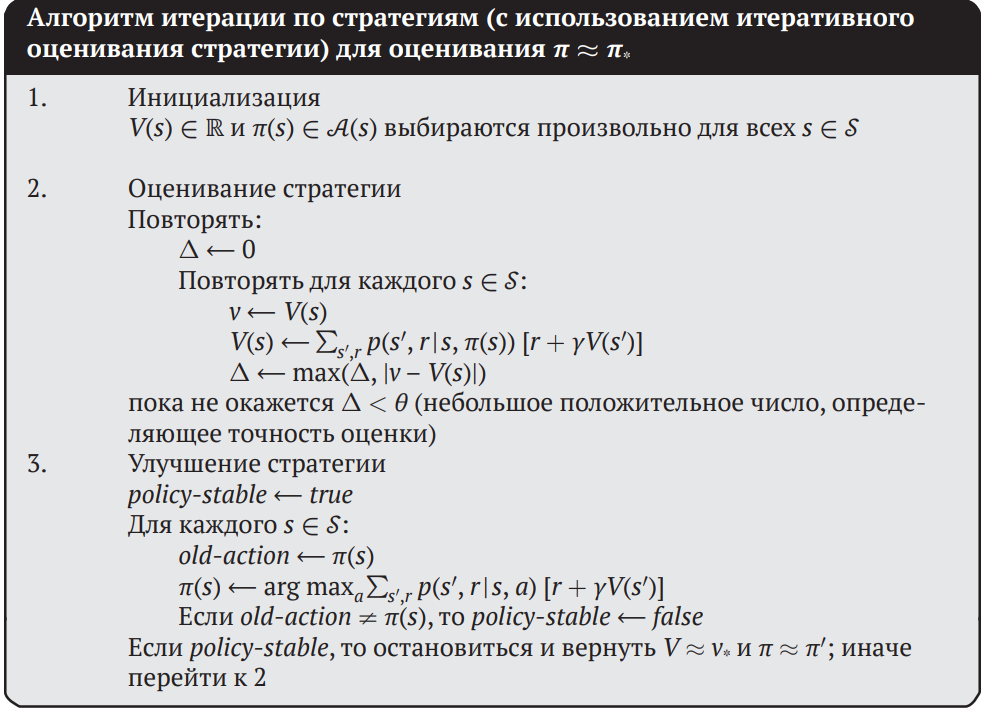
\includegraphics[width=1\linewidth]{iter_alg.png}
    \caption{}
\end{figure}
\begin{solution}
    Проблема возникает на этапе улучшения стратегии. Если множество $A'(s) = \text{Arg} \max_{a \in A(s)}
    q_{\pi}(s,a)$  состоит более чем из одного элемента и содержит $\pi(s)$, то нерегламентированный выбор действия ведет к появлению циклов. \\
    Поэтому в процесс улучшения стратегии следует добавить следующую проверку:
    \[
    \text{Если} \ \pi(s) \in A'(s), \ \text{то} \ \pi(s) \leftarrow \pi(s) \]
    \[
    \text{В противном случае } \pi(s) \leftarrow \forall a \in A'(s)
    \]
\end{solution}

\subsection{Упражнение 4.5(c. 111)}
Как следовало бы определить алгоритм итерации по стратегиям
для ценностей действий? Приведите полный алгоритм вычисления $q_*$, аналогичный показанному на стр. 110 для вычисления $v_*$. Обратите особое внимание на это упражнение, потому что развиваемые в нем идеи будут использоваться в книге далее. 
\begin{solution}
    Оценивание стратегии в терминах ценности действий приведено в упражнении 4.3. \\
    Заметим, что обновление стратегии по правилу
    \[\pi'(s) = \arg\max_aq_{\pi}(s, a)\]
    при известной ценности действий еще проще и не требует дополнительных равенств. \\
    Надо показать, что имеет место строгое улучшение стратегий:
    рассмотрим две детерминированные стратегии $\pi$ и $\pi'$ такие, что \[\pi'(s) = \arg\max_aq_{\pi}(s, a)\] 
    Предположим, что улучшения политики не произошло, тогда $q_{\pi'}(s,a) = q_{\pi}(s,a)$.
    Получим
    \[\pi'(s) = \arg\max_aq_{\pi}(s, a) = 
    \arg\max_aq_{\pi'}(s, a) \]
    Запишем уравнение Беллмана:
    \begin{align*}
        q_{\pi'}(s,a) = \\
        =& \sum_{s'\in S}\sum_{r\in R} p(s',r\mid s,a)\,\Bigl(r + \gamma\sum_{a'\in A(s')} \pi'(a'\mid s')\, q_{\pi'}(s',a')\Bigr) =\\
        =& \sum_{s'\in S}\sum_{r\in R} p(s',r\mid s,a)\,\Bigl(r + \gamma \cdot q_{\pi'}(s',\pi'(s'))\Bigr) =\\
        =& \sum_{s'\in S}\sum_{r\in R} p(s',r\mid s,a)\,\Bigl(r + \gamma \cdot \max_{a'} q_{\pi'}(s',a')\Bigr)
    \end{align*}
    Крайние равенства соответствуют уравнению оптимальности Беллмана, поэтому $q_{\pi'}(s,a) = q_{\pi}(s,a) = q_*(s,a)$ и $\pi(s) = \pi'(s) = \pi_*(s)$.
    \vspace{5mm} \\
    Псевдокод алгоритма: \\
    \textbf{Вход:} множества $S,\ A(s)$, динамика $p(s',r\mid s,a)$, $\gamma\in[0,1)$, порог $\theta>0$.\\
    \textbf{Выход:} $q_*$ и оптимальная стратегия $\pi_*$.
    
    \textbf{1. Инициализация}\\
    Для всех $s\in S$ выбрать $\pi(s)\in A(s)$ произвольно.\\
    Задать $q(s,a)$ произвольно для всех $(s,a)$.
    
    \textbf{2. Оценивание стратегии (итеративное)}\\
    \textbf{Повторять:}\\
    \hspace*{5mm} $\Delta \leftarrow 0$\\
    \hspace*{5mm} \textbf{для каждого } $s\in S$ \textbf{и каждого } $a\in A(s)$:\\
    \hspace*{5mm}\hspace*{5mm} $old \leftarrow q(s,a)$\\
    \hspace*{5mm}\hspace*{5mm} $q(s,a)\leftarrow 
    \sum_{s',r} p(s',r\mid s,a)\Bigl[r+\gamma\, q\bigl(s',\pi(s')\bigr)\Bigr]$\\
    \hspace*{5mm}\hspace*{5mm} $\Delta \leftarrow \max\bigl(\Delta,\ |old-q(s,a)|\bigr)$\\
    \textbf{пока } $\Delta \ge \theta$
    
    \textbf{3. Улучшение стратегии}\\
    $policy\_stable \leftarrow true$\\
    \textbf{для каждого } $s\in S$:\\
    \hspace*{5mm} $old\_action \leftarrow \pi(s)$\\
    \hspace*{5mm} $\pi(s)\leftarrow \arg\max_{a\in A(s)} q(s,a)$\\
    \hspace*{5mm} \textbf{если } $old\_action \ne \pi(s)$, \textbf{то } $policy\_stable \leftarrow false$\\
    \textbf{если } $policy\_stable$, \textbf{то остановиться и вернуть} $q, \ \pi$\\
    \textbf{иначе перейти к 2.}
\end{solution}

\subsection{Упражнение 4.6(c. 112)}
Предположим, что мы ограничены только $\varepsilon$-мягкими стратегиями, для которых вероятность выбора любого действия в каждом состоянии $s$ не меньше $\frac{\varepsilon}{|A(s)|}$. Качественно опишите изменения, которые нужно было бы внести
на шагах 3, 2 и 1 (именно в таком порядке) приведенного на стр. 110 алгоритма итерации по стратегиям для вычисления $v_*$.
\begin{solution}

    \textbf{3. Улучшение стратегии}\\
    policy-stable $\leftarrow$ true\\
    Для каждого $s \in S$:\\
    \hspace*{5mm} old-action $\leftarrow \arg\max_{a\in A(s)} \pi(a\mid s)$\\
    \hspace*{5mm} $a_* \leftarrow \arg\max_{a\in A(s)}
    \sum_{s',r} p(s',r\mid s,a)\bigl[r+\gamma V(s')\bigr]$\\
    \hspace*{5mm} Для каждого $a \in A(s)$:\\
    \hspace*{5mm}\hspace*{5mm} если $a=a_*$
    то 
    $\pi(a\mid s) \leftarrow 1-\varepsilon+\dfrac{\varepsilon}{|A(s)|}$\\
    \hspace*{5mm}\hspace*{5mm} иначе 
    $\pi(a\mid s) \leftarrow \dfrac{\varepsilon}{|A(s)|}$\\
    \hspace*{5mm} если old-action $\neq a_*$ то policy-stable $\leftarrow$ false\\
    Если policy-stable, то остановиться и вернуть $v_*$,$\pi_*$;
    иначе перейти к 2.
    
    \vspace{5mm}
    
    \textbf{2. Оценивание стратегии}\\
    Повторять: \\
    \hspace*{5mm} $\Delta \leftarrow 0$\\
    \hspace*{5mm} Повторять для каждого $s \in S$: \\
    \hspace*{5mm}\hspace*{5mm} $v \leftarrow V(s)$\\
    \hspace*{5mm}\hspace*{5mm} $V(s) \leftarrow 
    \sum_{a \in A(s)} \pi(a \mid s)
    \sum_{s',r} p(s', r \mid s, a)\,[r + \gamma V(s')]$\\
    \hspace*{5mm}\hspace*{5mm} $\Delta \leftarrow \max(\Delta,\ |v - V(s)|)$\\
    пока не окажется $\Delta < \theta$

    \vspace{5mm}

    \textbf{1. Инициализация}\\
    $V(s) \in \mathbb{R} \text{ выбираются произвольно для всех } s \in S$\\
    $\pi(a \mid s) \text{ выбирается произвольно при условии }
    \pi(a \mid s) \ge \dfrac{\varepsilon}{|A(s)|}
    \text{ для всех } s \in S \text{ и } a \in A(s)$
\end{solution}

\subsection{Упражнение 4.7(c. 112)}
Напишите программу, реализующую итерацию по стратегиям, и решите задачу об аренде машин со следующими изменениями. Один из служащих Джека в первом офисе каждую ночь ездит на автобусе домой, а живет он рядом со вторым офисом. Он с удовольствием готов
перегонять одну машину во второй офис бесплатно. Но каждая дополнительная машина все равно стоит 2 доллара, равно как и перегон всех машин в обратном направлении. Кроме того, в  каждом офисе у  Джека ограниченное количество парковочных мест. Если на ночь остается больше $10$ машин (после всех перегонов), то за пользование другой парковкой взимается дополнительно $4$ доллара
(вне зависимости от того, сколько машин там стоит). Такого рода нелинейности и  произвольная динамика часто встречаются в  реальных задачах, и  все методы оптимизации, кроме динамического программирования, к ним применимы с трудом. Для проверки своей программы сначала воспроизведите результаты
для исходной задачи.
\begin{solution}
    \textbf{Код смотри в отдельном файле репозитория.} \\
    Основную трудность составляет вычисление модели окружающей среды $p(s', r \mid s, a)$. Для более эффективных вычислений разобьем на два шага:
    \begin{equation}
    G(b_1,b_2) = \sum_{r_1,r_2}\mathbb{P}(r_1)\mathbb{P}(r_2)V(b_1+r_1,b_2+r_2)
    \tag{1}
    \end{equation}
    В этой формуле $b_1, b_2$ - ежедневное состояние офисов после запроса, но перед возвратом. Тогда $b_1 + r_1, b_2 + r_2$ - состояние офисов после возврата, где $r_1, r_2$ - всевозможные значения случайной величины возврата. Эта формула представляет собой математическо ожидание по возвратам(усредненная ценность) \\
    Рассмотрим второй шаг:
    \begin{equation}
    V(s_1,s_2) = \sum_{q_1,q_2}\mathbb{P}(q_1)\mathbb{P}(q_2)\left[r + \gamma G(b_1,b_2)\right]
    \tag{2}
    \end{equation}
    В этой формуле $s_1, s_2$ - состояние среды перед запросом, но после перегона, $q_1, q_2$ - запросы в первом и втором офисе соответственно, $b_1 = s_1 - q_1, b_2 = s_2 - q_2$ - ежедневное состояние офисов после запроса, но перед возвратом.
    По аналогии эта формула является усреднением ценности по запросам. Именно ей я пользуюсь в коде как при оценивании, так и при улучшении стратегии. \\
    В приложенном ноутбуке решается исходный пример, а после он модифицируется под упражнение. Некоторые области полученного графика не поддаются логическому объяснению. Я связываю это с произвольной и нелинейной динамикой.
    \begin{figure}[H]
    \centering

    \begin{subfigure}{0.48\textwidth}
        \centering
        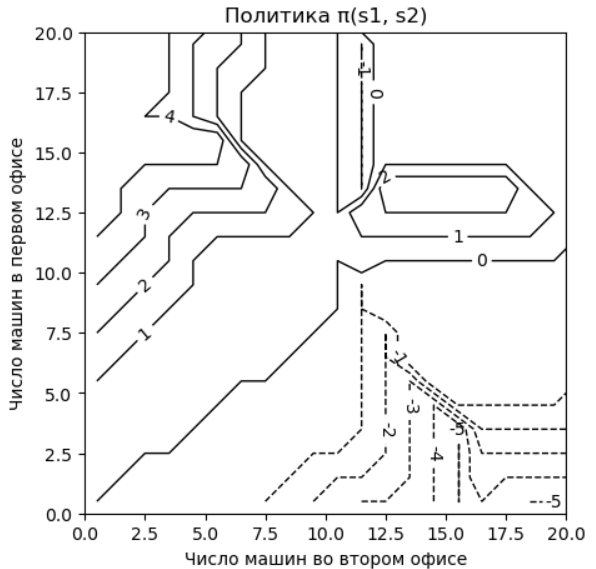
\includegraphics[width=\linewidth]{fig_4_7_final.png}
        \caption{Решение упр.4.7}
    \end{subfigure}
    \hfill
    \begin{subfigure}{0.48\textwidth}
        \centering
        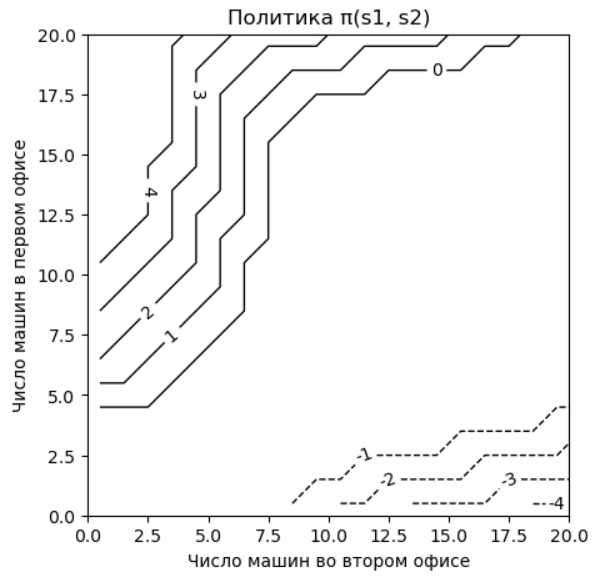
\includegraphics[width=\linewidth]{fig_4_7_sol.png}
        \caption{Решение исходного примера}
    \end{subfigure}

    \caption{Сравнение результатов}
    \end{figure}
\end{solution}

\subsection{Упражнение 4.8(c. 114)}
Почему у оптимальной политики в задаче игрока такая странная
форма? В частности, для капитала $50$ предлагается поставить все на одно подбрасывание, а для капитала $51$ - нет. Почему такая стратегия хороша? 
\begin{solution}
    Запишем формулу для оптимальной политики:
    \[\pi_*(s) = \arg\max_a\ \left[p_h\cdot V_*(s+a) + 
    (1 - p_h) \cdot V_*(s-a)\right]\]
    В условии задачи $p_h < 0.5$, поэтому игроку разумно действовать осторожно. При $s=51$ максимальная ставка равна $49$, но в случае неудачи, с вероятностью $0.6$, он окажется в состоянии $s=2$, ценность которого мала. Поэтому игрок выбирает поставить $1$ доллар и в худшем случае оказаться в состоянии $s=50$, которое является более оптимистичным.
\end{solution}

\subsection{Упражнение 4.9(c. 115)}
Реализуйте алгоритм итерации по ценности для задачи игрока и решите ее для $p_h = 0.25$ и $p_h= 0.55$. Возможно, вы сочтете удобным ввести два фиктивных состояния, соответствующих завершению с капиталом $0$ и $100$, сопоставив им ценности $0$ и $1$. Представьте свои результаты графически, как на рис.4.3. Является ли полученное решение устойчивым при 
$\theta \rightarrow  0$?
\begin{solution}
    \textbf{Код смотри в отдельном файле репозитория.} При $\theta \rightarrow  0$ оценивание политики сходится к единственной оптимальной функции ценности, но выбор действий в оптимальной политике определен не единственным образом(для сравнения результатов в коде я разрешал неоднозначности, выбирая минимальную ставку)
    \begin{figure}[H]
    \centering

    \begin{subfigure}{0.8\textwidth}
        \centering
        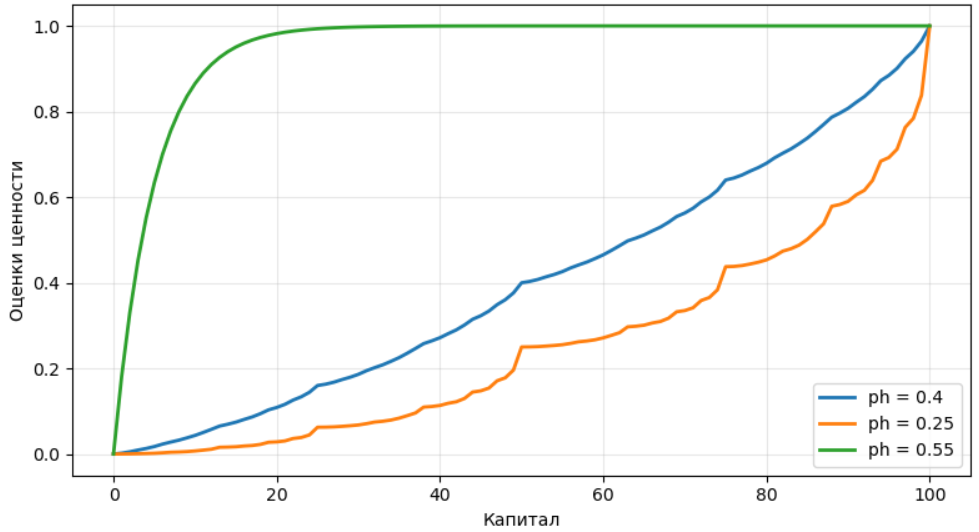
\includegraphics[width=\linewidth]{fig_4_9_sol_v.png}
        \caption{Оптимальная ценность состояний}
    \end{subfigure}
    \hfill
    \begin{subfigure}{0.8\textwidth}
        \centering
        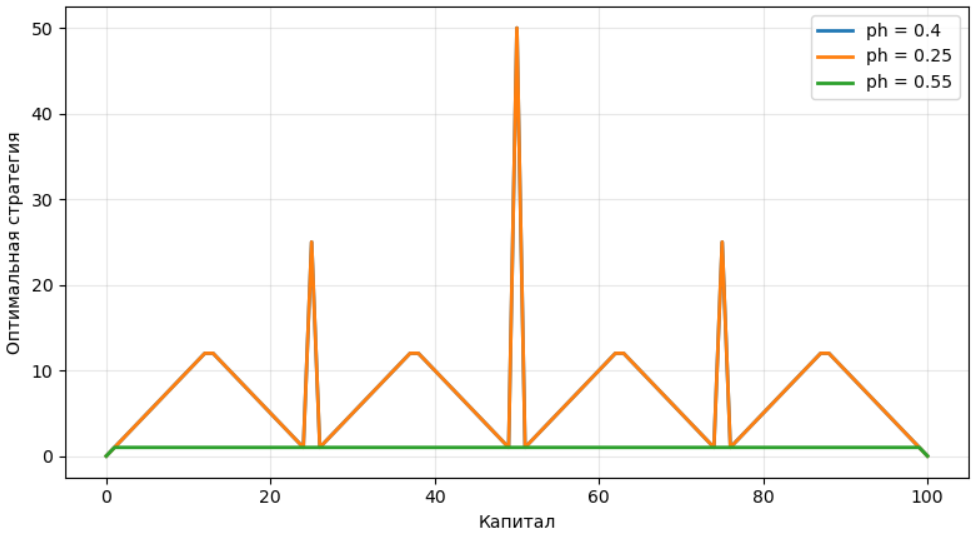
\includegraphics[width=\linewidth]{fig_4_9_pi.png}
        \caption{Оптимальная политика}
    \end{subfigure}

    \caption{}
    \end{figure}
\end{solution}

\subsection{Упражнение 4.10(c. 115)}
Каков аналог обновления в  алгоритме итерации по ценности
$(4.10)$ для ценностей действий $q_{k+1}(s, a)$? 
\begin{align*}
    v_{k+1}(s) &= \\
    &=\max_a\mathbb{E}\left[ R_{t+1}+\gamma\cdot v_{k}(S_{t+1} )\mid S_t=s, A_t=a) \right] =\\
    &= \max_a\sum_{s',r}p(s',r\mid s,a)\cdot\left[r + \gamma\cdot v_k(s')\right]
\tag{4.10}
\end{align*}
\begin{solution}
    Как и в случае ценности состояний, эта формула следует либо из упражнения 4.5, либо из уравнения оптимальности Беллмана для ценности действий:
    \[
        q_{k+1}(s,a)
        =
        \sum_{s',r}
        p(s',r \mid s,a)
        \left[
        r + \gamma \max_{a'} q_k(s', a')
        \right]
    \]
\end{solution}

\section{Глава 5. Методы Монте-Карло}
\subsection{Упражнение 5.1(c. 126)}
Рассмотрим диаграммы на рис. $5.1$ справа. Почему оценка функции ценности резко возрастает в последних двух строках на заднем плане? Почему она спадает в последней строке на диаграмме слева? Почему значения на переднем плане на верхних диаграммах выше, чем на нижних? 
\begin{figure}[H]
    \centering
    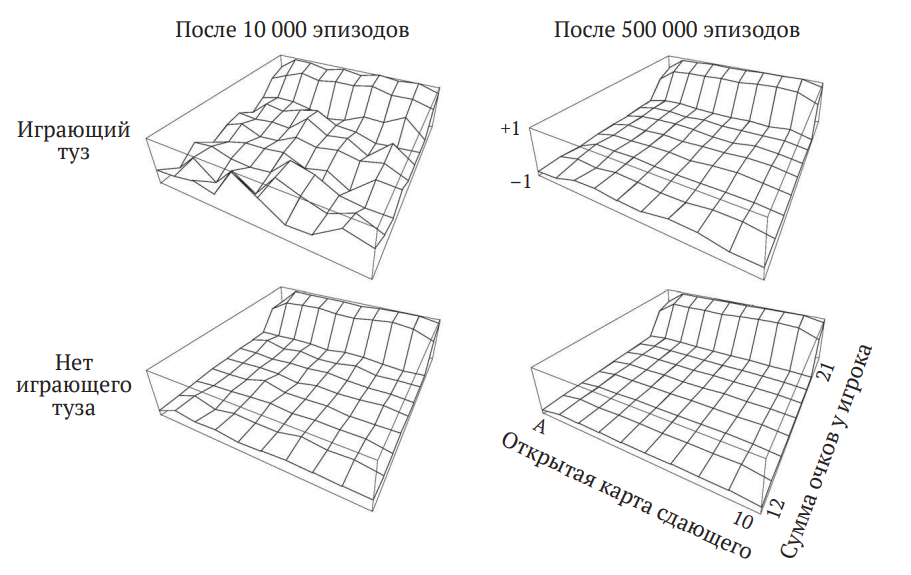
\includegraphics[width=1\linewidth]{fig_5_1.png}
    \caption{Рис. 5.1. Приближенные функции ценности состояний для стратегии игры в блэкджек, при которой игрок останавливается, набрав $20$ или $21$. Вычислены посредством оценивания стратегии методом Монте-Карло.}
\end{figure}
\begin{solution}
    \begin{enumerate}
        \item Из условия задачи очевидно, что стратегия игрока далеко не оптимальна: дойти до суммы $20$ или $21$ сложно без "перебора". Но в случае достижения таких значений выигрыш практически гарантирован, поэтому ценность состояний резко возрастает на последних двух строках.
        \item Левая строка соответствует случаю, когда открытой картой сдающего является туз. Это самый выгодный случай для противника, поэтому ценность состояний падает в этой строке.
        \item Ценность состояний при наличии играющего туза больше ценности состояний в случае его отсутствия, потому что играющий туз дает игроку запасной шанс: при переборе можно засчитать туз за $1$ и продолжить игру.
    \end{enumerate}
\end{solution}

\subsection{Упражнение 5.2(c. 126)}
Предположим, что вместо МК первого посещения для моделирования игры в блэкджек использовался МК всех посещений. Как вы думаете, будет ли результат сильно отличаться? Объясните свой ответ. 
\begin{solution}
    Не будет, так как внутри одного эпизода состояния повторяться не могут(так как сумма очков у игрока может только увеличиться). Это означает, что первое посещение состояния будет единственным. Небольшие различия могут быть обусловлены шумом.
\end{solution}

\subsection{Упражнение 5.3(c. 128)}
Нарисуйте диаграмму предшествующих состояний для оценивания $q_{\pi}$ методом Монте-Карло. 
\begin{solution}
    \leavevmode

    \medskip
    \centering
    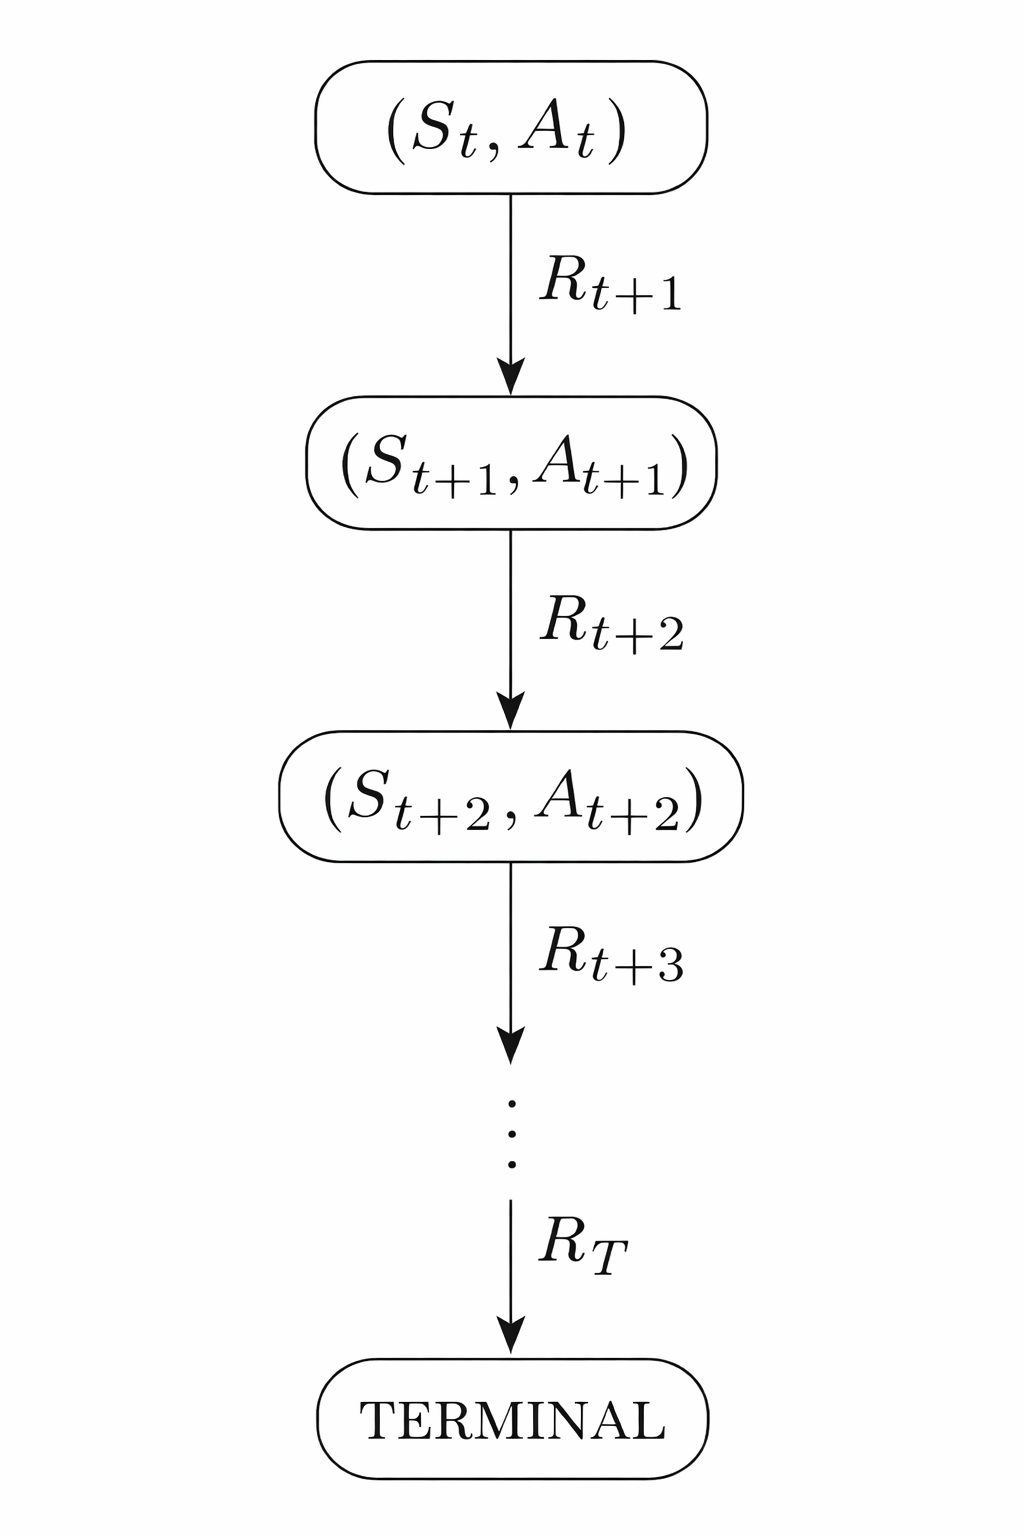
\includegraphics[width=0.4\linewidth]{fig_5_3_sol.png}

    \captionof{figure}{
    По аналогии с функциями ценности состояний теперь мы оцениваем пару состояние-действие, которая зависит от следующих пар до конца эпизода. Ветвления нет, потому что мы считаем доход по эпизоду.
    }
    \label{fig:5_3_sol}
\end{solution}

\subsection{Упражнение 5.4(c. 131)}
Псевдокод метода Монте-Карло ИС не эффективен, потому что для каждой пары состояние–действие он хранит список всех доходов и повторно вычисляет среднее. Было бы эффективнее использовать описанную в разделе 2.4
технику – хранить только среднее и количество элементов в списке (для каждой пары состояние–действие) и обновлять их инкрементно. Покажите, как для этого следует модифицировать псевдокод.
\begin{solution}
    \leavevmode\\
    \begin{algorithm}[H]
    \SetAlgoLined
    \DontPrintSemicolon
    \caption{Метод Монте-Карло ИС (с исследовательскими стартами), инкрементная версия}

    \textbf{Инициализация:}\;
    \Indp
    $\pi(s) \in \mathcal{A}(s)$ (произвольная) для всех $s \in \mathcal{S}$\;
    $Q(s, a) \in \mathbb{R}$ (произвольная) для всех $s \in \mathcal{S},\ a \in \mathcal{A}(s)$\;
    $N(s, a) \leftarrow 0$ для всех $s \in \mathcal{S},\ a \in \mathcal{A}(s)$\;
    \Indm

    \BlankLine
    \textbf{Повторять бесконечно (для каждого эпизода):}\;
    \Indp
    Выбрать $S_0 \in \mathcal{S},\ A_0 \in \mathcal{A}(S_0)$ случайным образом, так что вероятность любой пары больше 0\;
    Сгенерировать эпизод, начинающийся в $S_0, A_0$ и следующий $\pi$:\;
    \quad $S_0, A_0, R_1, \ldots, S_{T-1}, A_{T-1}, R_T$\;
    $G \leftarrow 0$\;
    \For{$t = T-1, T-2, \ldots, 0$}{
        $G \leftarrow \gamma G + R_{t+1}$\;
        \If{пара $S_t, A_t$ не встречается в $S_0, A_0, S_1, A_1, \ldots, S_{t-1}, A_{t-1}$}{
            $N(S_t, A_t) \leftarrow N(S_t, A_t) + 1$\;
            $Q(S_t, A_t) \leftarrow Q(S_t, A_t) + \dfrac{1}{N(S_t, A_t)}\bigl(G - Q(S_t, A_t)\bigr)$\;
            $\pi(S_t) \leftarrow \arg\max_a Q(S_t, a)$\;
        }
    }
    \Indm

    \end{algorithm}
\end{solution}

\subsection{Упражнение 5.5(c. 138)}
Рассмотрим МППР с одним незаключительным состоянием и одним действием, которое ведет назад в незаключительное состояние с вероятностью $p$ и в заключительное состояние с вероятностью $1 - p$. Пусть вознаграждение
за любой переход равно $+1$ и $\gamma = 1$. Предположим, что наблюдается один эпизод,
продолжающийся $10$ шагов, с доходом $10$. Каковы оценки ценности незаключительного состояния в случае первого посещения и всех посещений? 
\begin{solution}
    Эпизод длиной $10$ шагов с доходом $G = 10$ имеет вид:

    \begin{center}
    \resizebox{\textwidth}{!}{%
    \begin{tikzpicture}[
        every node/.style={font=\small},
        state/.style={circle, draw, thick, minimum size=7mm, inner sep=1pt},
        terminal/.style={rectangle, draw, thick, minimum size=7mm, inner sep=2pt, fill=gray!20},
        arrow/.style={-{Stealth[length=2mm]}, thick}
    ]
    \foreach \i in {0,...,9} {
        \node[state] (s\i) at (\i*1.4, 0) {$s$};
        \node[below=1mm of s\i] {\scriptsize $t=\i$};
    }
    \node[terminal] (term) at (14, 0) {\scriptsize term};
    \node[below=1mm of term] {\scriptsize $t=10$};
    \foreach \i [evaluate=\i as \j using int(\i+1)] in {0,...,8} {
        \draw[arrow] (s\i) -- node[above, font=\scriptsize] {$+1$} (s\j);
    }
    \draw[arrow] (s9) -- node[above, font=\scriptsize] {$+1$} (term);
    \end{tikzpicture}%
    }
    \end{center}

    При $\gamma = 1$ доход с момента $t$ равен $G_t = 10 - t$.

    \textbf{First-visit MC:} учитывается только первое посещение ($t = 0$):
    \[
    V_{\text{first-visit}}(s) = G_0 = 10.
    \]

    \textbf{Every-visit MC:} усредняются доходы со всех $10$ посещений:
    \[
    V_{\text{every-visit}}(s) = \frac{10 + 9 + \cdots + 1}{10} = \frac{55}{10} = 5{,}5.
    \]
\end{solution}

\subsection{Упражнение 5.6(c. 141)}
Как выглядит уравнение, аналогичное $(5.6)$, если вместо ценностей состояний $V(s)$ использовать ценности действий $Q(s, a)$, опять-таки при известных доходах, сгенерированных с помощью стратегии $b$?
\begin{solution}
    В формуле (5.6) для оценки $V(s)$:
    \[
    V(s) \doteq \frac{\sum_{t \in \mathcal{T}(s)} \rho_{t:T(t)-1}\, G_t}{\sum_{t \in \mathcal{T}(s)} \rho_{t:T(t)-1}}
    \]
    нужно сделать две замены.

    \textbf{1. Множество индексов.} Вместо $\mathcal{T}(s)$ — моментов посещения состояния $s$ — берём
    \[
    \mathcal{T}(s,a) = \{t : S_t = s,\ A_t = a\}.
    \]

    \textbf{2. Коэффициент $\rho$ начинается с шага $t+1$.} Действие $A_t = a$
    зафиксировано условием, поэтому отношение $\pi(A_t \mid S_t) / b(A_t \mid S_t)$
    для шага $t$ в коэффициент не входит — корректировать нужно только то, что
    происходит после этого выбора:
    \[
    \rho_{t+1:T(t)-1} = \prod_{k=t+1}^{T(t)-1} \frac{\pi(A_k \mid S_k)}{b(A_k \mid S_k)}.
    \]

    \textbf{Итоговая формула:}
    \[
    \boxed{\,Q(s,a) \doteq \frac{\sum_{t \in \mathcal{T}(s,a)} \rho_{t+1:T(t)-1}\, G_t}{\sum_{t \in \mathcal{T}(s,a)} \rho_{t+1:T(t)-1}}\,}
    \]
\end{solution}

\subsection{Упражнение 5.7(c. 141)}
На кривых обучения типа показанных на рис. $5.3$ ошибка обычно убывает по мере обучения, как и случилось для метода обыкновенной выборки по значимости. Но для метода взвешенной выборки по значимости ошибка сначала
возрастает, а потом убывает. Как вы думаете, почему так происходит?
\begin{figure}[H]
    \centering
    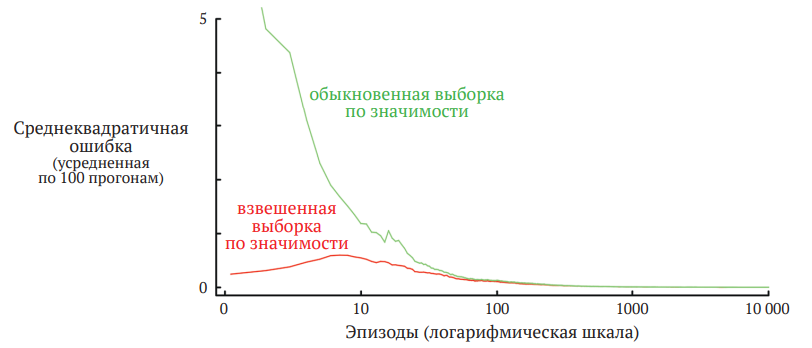
\includegraphics[width=1\linewidth]{fig_5_3.png}
    \caption{Рис. 5.3. Взвешенная выборка по значимости дает меньшую ошибку оценки ценности одного состояния в блэкджеке по эпизодам с разделенной стратегией}
\end{figure}
\begin{solution}
    Оценка инициализируется нулём, что близко к истинной ценности $-0{,}27726$,
    поэтому начальная ошибка мала. Поведенческая стратегия выбирает «ещё» и
    «хватит» равновероятно, тогда как целевая всегда останавливается, поэтому
    эпизоды с ненулевым $\rho$ редки.

    Пока все наблюдённые $\rho_t = 0$, знаменатель нулевой и оценка остаётся
    равной начальному значению $0$. Как только появляется первый эпизод с
    $\rho > 0$, веса в формуле
    \[
    V(s) = \frac{\sum_t \rho_t\, G_t}{\sum_t \rho_t}
    \]
    сокращаются, и оценка становится равна доходу этого единственного эпизода:
    \[
    V(s) = \frac{\rho_1 G_1}{\rho_1} = G_1 \in \{-1, 0, +1\}.
    \]
    Прыжок от $0$ к $\pm 1$ резко увеличивает квадратичную ошибку относительно
    истинного значения $-0{,}28$. По мере накопления согласующихся эпизодов
    оценка усредняется и подтягивается к истинной ценности — ошибка убывает.

    Иными словами, всплеск возникает потому, что взвешенная оценка по одному
    эпизоду полностью игнорирует вес и сводится к самому доходу, что временно
    уводит её от истинной ценности.
\end{solution}

\subsection{Упражнение 5.8(c. 141)}
При получении результатов в примере $5.5$, показанных на рис. $5.4$,
использовался метод МК первого посещения. Допустим, что для той же задачи был
применен метод МК всех посещений. Будет ли в таком случае дисперсия оценки
по-прежнему бесконечной? Объясните свой ответ.
\begin{figure}[H]
    \centering
    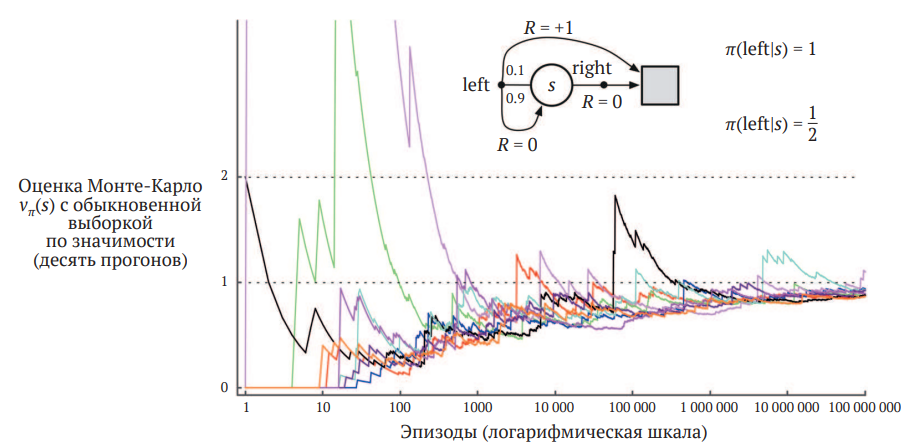
\includegraphics[width=1\linewidth]{fig_5_4.png}
    \caption{Рис. 5.4. Обыкновенная выборка по значимости порождает на удивление неустойчивые оценки для МППР с  одним состоянием, показанным
    в верхней части (пример 5.5). В данном случае правильная оценка равна 1
    $(\gamma = 1)$, но, хотя это действительно математическое ожидание выборочного дохода (после выборки по значимости), дисперсия выборки бесконечна
    и оценки не сходятся к этому значению. Эти результаты имеют место для МК
    первого посещения с разделенной стратегией
    }
\end{figure}
\begin{solution}
    Дисперсия по-прежнему бесконечна.

    В методе всех посещений каждый эпизод даёт вклад в $\mathbb{E}_b[\rho^2 G^2]$
    от \emph{каждого} посещения состояния $s$, тогда как в методе первого
    посещения учитывается только посещение в момент $t = 0$. Слагаемое от
    первого посещения в обоих методах одно и то же, а в методе всех посещений
    к нему добавляются дополнительные слагаемые от посещений в моменты
    $t = 1, 2, \ldots$

    Все слагаемые неотрицательны ($\rho^2 \geq 0$, $G^2 \geq 0$), поэтому
    $\mathbb{E}_b[\rho^2 G^2]$ для метода всех посещений не меньше, чем для
    метода первого посещения. Поскольку в учебнике для first-visit получен
    расходящийся ряд $0{,}2\sum_{k=0}^\infty 1{,}8^k = \infty$, больший по
    членам ряд для every-visit расходится тем более — дисперсия остаётся
    бесконечной.
\end{solution}

\subsection{Упражнение 5.9(c. 142)}
Модифицируйте алгоритм для оценивания стратегии методом МК первого посещения (раздел $5.1$), воспользовавшись инкрементной реализацией выборочного среднего, описанной в разделе $2.4$.
\begin{solution}
    \leavevmode\\
    \begin{algorithm}[H]
    \SetAlgoLined
    \DontPrintSemicolon
    \caption{Предсказание методом МК первого посещения для оценивания $V \approx v_\pi$ (инкрементная версия)}

    \KwIn{стратегия $\pi$, подлежащая оцениванию}

    \textbf{Инициализация:}\;
    \Indp
    $V(s) \in \mathbb{R}$ (произвольная) для всех $s \in \mathcal{S}$\;
    $N(s) \leftarrow 0$ для всех $s \in \mathcal{S}$\;
    \Indm

    \BlankLine
    \textbf{Повторять бесконечно (для каждого эпизода):}\;
    \Indp
    Сгенерировать эпизод, следуя $\pi$: $S_0, A_0, R_1, S_1, A_1, R_2, \ldots, S_{T-1}, A_{T-1}, R_T$\;
    $G \leftarrow 0$\;
    \For{$t = T-1, T-2, \ldots, 0$}{
        $G \leftarrow \gamma G + R_{t+1}$\;
        \If{$S_t$ не встречается в $S_0, S_1, \ldots, S_{t-1}$}{
            $N(S_t) \leftarrow N(S_t) + 1$\;
            $V(S_t) \leftarrow V(S_t) + \dfrac{1}{N(S_t)}\bigl(G - V(S_t)\bigr)$\;
        }
    }
    \Indm

    \end{algorithm}
\end{solution}

\subsection{Упражнение 5.10(c. 143)}
Выведите правило обновления взвешенного среднего $(5.8)$ из
$(5.7)$. Рассуждайте так же, как при выводе правила для обычного среднего $(2.3)$.
\begin{equation}
    V_n \doteq \frac{\sum_{k=1}^{n-1} W_k G_k}{\sum_{k=1}^{n-1} W_k}, \quad n \geq 2,
    \tag{5.7}
\end{equation}
\begin{equation}
    V_{n+1} \doteq V_n + \frac{W_n}{C_n}\bigl[G_n - V_n\bigr], \quad n \geq 1,
    \tag{5.8}
\end{equation}
\begin{solution}
    Обозначим $C_n = \sum_{k=1}^{n} W_k$. Тогда из $(5.7)$:
    \[
    V_{n+1} = \frac{\sum_{k=1}^{n} W_k G_k}{C_n} = \frac{\sum_{k=1}^{n-1} W_k G_k + W_n G_n}{C_n}.
    \]
    Заметим, что $\sum_{k=1}^{n-1} W_k G_k = C_{n-1} V_n$, поэтому
    \[
    V_{n+1} = \frac{C_{n-1} V_n + W_n G_n}{C_n} = \frac{(C_n - W_n) V_n + W_n G_n}{C_n} = V_n + \frac{W_n}{C_n}\bigl[G_n - V_n\bigr].
    \]
\end{solution}

\subsection{Упражнение 5.11(c. 144)}
В приведённом выше алгоритме управления методом МК с разделённой стратегией вы, возможно, ожидали, что в обновлении $W$ будет участвовать коэффициент выборки по значимости $\pi(A_t \mid S_t) / b(A_t \mid S_t)$, а на самом деле мы видим $1/b(A_t \mid S_t)$. Почему же, несмотря на это, алгоритм корректен?
\begin{solution}
    Целевая стратегия $\pi$ детерминирована и жадна: $\pi(s) = \arg\max_a Q(s, a)$. Поэтому $\pi(A_t \mid S_t)$ принимает лишь два значения:
    \[
    \pi(A_t \mid S_t) = 
    \begin{cases}
        1, & \text{если } A_t = \pi(S_t), \\
        0, & \text{если } A_t \neq \pi(S_t).
    \end{cases}
    \]
    В случае $A_t \neq \pi(S_t)$ весь коэффициент $\rho$ обнуляется, и вклад в обновление становится нулевым. В оставшемся случае $A_t = \pi(S_t)$ выполнено $\pi(A_t \mid S_t) = 1$, поэтому
    \[
    \frac{\pi(A_t \mid S_t)}{b(A_t \mid S_t)} = \frac{1}{b(A_t \mid S_t)}.
    \]
\end{solution}

\subsection{Упражнение 5.12. Кольцевые гонки(c. 145)}
Рассмотрим
управление гоночным автомобилем на повороте, показанном на рис.  $5.5$. Вы
хотите пройти его как можно быстрее, но не настолько быстро, чтобы вылететь
с трассы. В нашей упрощенной модели кольцевых гонок автомобиль может находиться в одной из дискретных ячеек сетки. Скорость также дискретна и равна
количеству ячеек, на которые машина переместилась по горизонтали и по вертикали за один временной шаг. Действия – приращения составляющих скорости.
Каждая может изменяться на $+1, -1$ или $0$ на одном шаге, так что всего имеется
девять $(3 \times 3)$ действий. Обе составляющие скорости должны быть неотрицательны и меньше $5$, и одновременно могут быть равны $0$ только на линии старта. Каждый эпизод начинается в одном из случайно выбранных начальных состояний,
когда обе составляющие скорости равны нулю, а  заканчивается, когда машина
пересечет линию финиша. За каждый шаг до пересечения линии финиша полагается вознаграждение $-1$. Если машина задела границу трассы, то она возвращается
в случайную позицию на линии старта, обе составляющие скорости обнуляются,
и  эпизод продолжается. Прежде чем обновлять положение машины на каждом
шаге, следует проверить, не пересекает ли предполагаемая траектория движения
границу трассы. Если машина пересекает линию финиша, то эпизод заканчивается; если она пересекает какую-то другую границу, то считается, что машина вылетела с трассы, поэтому она возвращается на линию старта. Чтобы сделать задачу
более интересной, с вероятностью $0.1$ на каждом временном шаге оба приращения, составляющих скорости, равны нулю независимо от того, какими они должны
были бы стать. Примените к этой задаче метод управления Монте-Карло, чтобы
вычислить оптимальную стратегию при старте из каждого начального состояния.
Нарисуйте несколько траекторий, следующих оптимальной стратегии (но подавите для них шум).
\begin{figure}[H]
    \centering
    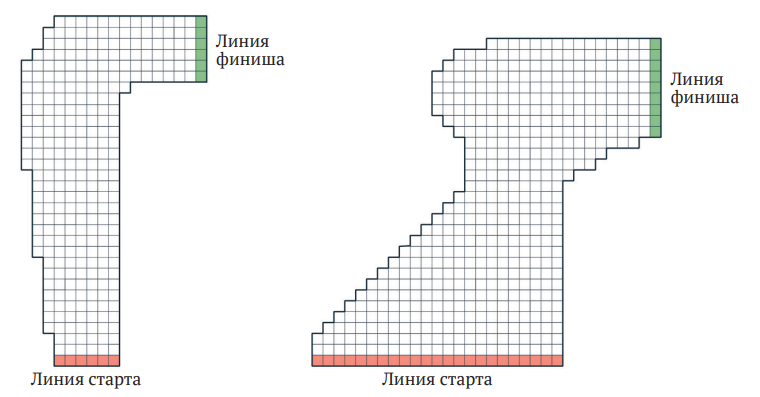
\includegraphics[width=0.6\linewidth]{fig_5_5.png}
    \caption{Рис. 5.5. Два правых поворота в задаче о круговых гонках}
\end{figure}
\begin{solution}
    \textbf{Код смотри в отдельном файле репозитория.} \\
    \begin{figure}[H]
    \centering
    \begin{minipage}{0.4\textwidth}
        \centering
        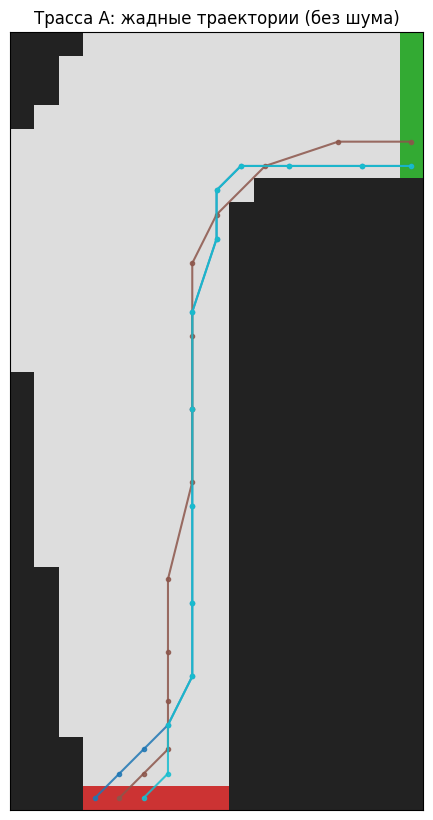
\includegraphics[width=\linewidth]{track_a.png}
    \end{minipage}\hfill
    \begin{minipage}{0.4\textwidth}
        \centering
        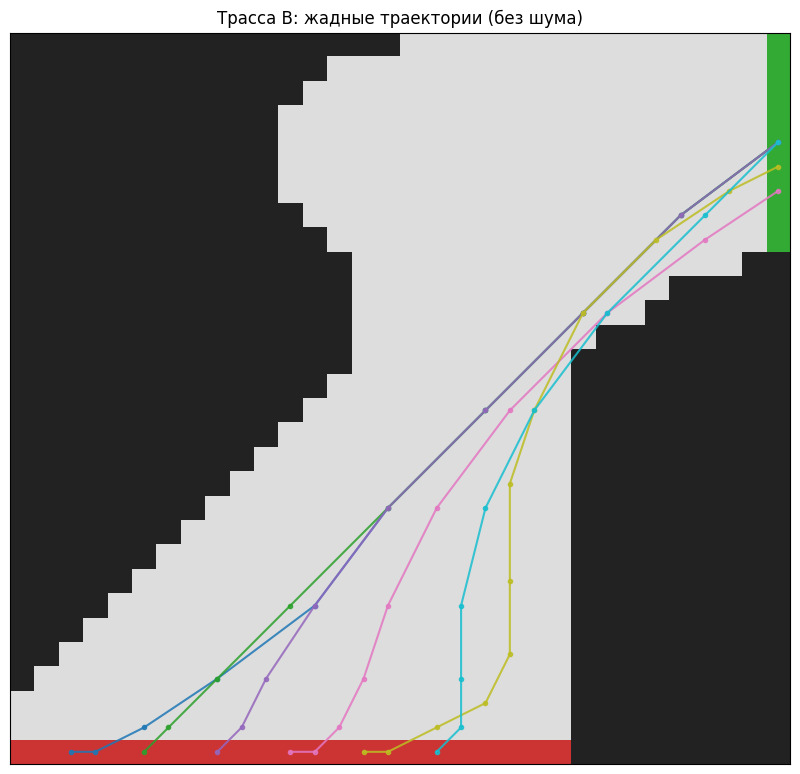
\includegraphics[width=\linewidth]{track_b.png}
    \end{minipage}
    \end{figure}
\end{solution}


\subsection{*Упражнение 5.13(c. 148)}
Восполните шаги, необходимые для вывода $(5.14)$ из $(5.12)$.
\begin{equation}
    \resizebox{0.8\textwidth}{!}{$\displaystyle \rho_{t:T-1} R_{t+1} = \frac{\pi(A_t|S_t)}{b(A_t|S_t)} \frac{\pi(A_{t+1}|S_{t+1})}{b(A_{t+1}|S_{t+1})} \frac{\pi(A_{t+2}|S_{t+2})}{b(A_{t+2}|S_{t+2})} \cdots \frac{\pi(A_{T-1}|S_{T-1})}{b(A_{T-1}|S_{T-1})} R_{t+1}. $}
    \tag{5.12}
\end{equation}
\begin{equation}
    \mathbb{E}[\rho_{t:T-1} R_{t+1}] = \mathbb{E}[\rho_{t:t} R_{t+1}].
    \tag{5.14}
\end{equation}
\begin{solution}
    Подставляя $(5.12)$ в левую часть $(5.14)$, получаем:
    \[
    \mathbb{E}[\rho_{t:T-1} R_{t+1}] = \mathbb{E}\left[\frac{\pi(A_t|S_t)}{b(A_t|S_t)} R_{t+1} \cdot \prod_{k=t+1}^{T-1} \frac{\pi(A_k|S_k)}{b(A_k|S_k)}\right].
    \]
    Матожидание произведения распадается на произведение матожиданий:
    \[
    = \mathbb{E}[\rho_{t:t} R_{t+1}] \cdot \prod_{k=t+1}^{T-1} \mathbb{E}\left[\frac{\pi(A_k|S_k)}{b(A_k|S_k)}\right].
    \]
    По $(5.13)$ каждый множитель при $k \geq t+1$ равен $1$, откуда
    \[
    \mathbb{E}[\rho_{t:T-1} R_{t+1}] = \mathbb{E}[\rho_{t:t} R_{t+1}]. 
    \]
\end{solution}

\subsection{*Упражнение 5.14(c. 148)}
Модифицируйте алгоритм управления Монте-Карло с разделённой стратегией (стр.~144), воспользовавшись идеей усечённой средневзвешенной оценки $(5.10)$. Заметим, что сначала нужно будет преобразовать это равенство, введя ценности действий.
\begin{equation}
    \resizebox{0.85\linewidth}{!}{$\displaystyle V(s) \doteq \frac{\sum_{t \in \mathcal{T}(s)} \left((1-\gamma)\sum_{h=t+1}^{T(t)-1} \gamma^{h-t-1} \rho_{t:h-1} \bar{G}_{t:h} + \gamma^{T(t)-t-1} \rho_{t:T(t)-1} \bar{G}_{t:T(t)}\right)}{\sum_{t \in \mathcal{T}(s)} \left((1-\gamma)\sum_{h=t+1}^{T(t)-1} \gamma^{h-t-1} \rho_{t:h-1} + \gamma^{T(t)-t-1} \rho_{t:T(t)-1}\right)}. $}
    \tag{5.10}
\end{equation}
\begin{solution}
    \textbf{Преобразование $(5.10)$ для ценностей действий.}
    Действие $A_t = a$ задано условием, поэтому importance ratio начинаются с $\rho_{t+1:\cdot}$. Выделим слагаемое $h = t+1$ из внутренней суммы (для него $\bar{G}_{t:t+1} = R_{t+1}$ и importance ratio отсутствует):
    \[
    \resizebox{0.97\linewidth}{!}{$\displaystyle Q(s,a) \doteq \frac{\sum_{t \in \mathcal{T}(s,a)} \left((1-\gamma) R_{t+1} + (1-\gamma)\sum_{h=t+2}^{T(t)-1} \gamma^{h-t-1} \rho_{t+1:h-1} \bar{G}_{t:h} + \gamma^{T(t)-t-1} \rho_{t+1:T(t)-1} \bar{G}_{t:T(t)}\right)}{\sum_{t \in \mathcal{T}(s,a)} \left((1-\gamma) + (1-\gamma)\sum_{h=t+2}^{T(t)-1} \gamma^{h-t-1} \rho_{t+1:h-1} + \gamma^{T(t)-t-1} \rho_{t+1:T(t)-1}\right)}. $}
    \]

    \textbf{Рекуррентные соотношения.}
    Обозначим числитель и знаменатель добавки от момента $t$ как $N_t$ и $D_t$. Используя $\bar{G}_{t:h} = R_{t+1} + \bar{G}_{t+1:h}$, получаем:
    \[
    \begin{aligned}
    N_t &= R_{t+1} \cdot D_t + \gamma \rho_{t+1} N_{t+1}, \\
    D_t &= (1-\gamma) + \gamma \rho_{t+1} D_{t+1},
    \end{aligned}
    \]
    где
    \[
    \rho_{t+1} = \frac{\pi(A_{t+1}\mid S_{t+1})}{b(A_{t+1}\mid S_{t+1})},
    \qquad N_{T-1} = R_T, \qquad D_{T-1} = 1.
    \]

    \noindent\textbf{Алгоритм.}
    \par\noindent
    \begin{algorithm}[H]
        \DontPrintSemicolon
        \SetAlgoLined
        \KwIn{Поведенческая политика $b$ с покрытием $\pi$}
        \KwOut{Целевая политика $\pi \approx \pi_*$}
        \BlankLine
        \textbf{Инициализация:}\;
        \For{всех $s \in \mathcal{S}$, $a \in \mathcal{A}(s)$}{
            $Q(s,a) \leftarrow$ произвольно\;
            $C_{\text{num}}(s,a) \leftarrow 0$, $\quad C_{\text{den}}(s,a) \leftarrow 0$\;
        }
        $\pi(s) \leftarrow \arg\max_a Q(s,a)$ для всех $s \in \mathcal{S}$\;
        \BlankLine
        \ForEach{эпизод}{
            Сгенерировать эпизод по $b$: $S_0, A_0, R_1, \ldots, S_{T-1}, A_{T-1}, R_T$\;
            $N \leftarrow 0$, $\quad D \leftarrow 0$\;
            \For{$t = T-1, T-2, \ldots, 0$}{
                \eIf{$t = T-1$}{
                    $N \leftarrow R_{t+1}$, $\quad D \leftarrow 1$\;
                }{
                    $\rho \leftarrow \dfrac{\pi(A_{t+1}\mid S_{t+1})}{b(A_{t+1}\mid S_{t+1})}$\;
                    $N \leftarrow R_{t+1} \cdot D + \gamma \cdot \rho \cdot N$\;
                    $D \leftarrow (1-\gamma) + \gamma \cdot \rho \cdot D$\;
                }
                $C_{\text{num}}(S_t, A_t) \leftarrow C_{\text{num}}(S_t, A_t) + N$\;
                $C_{\text{den}}(S_t, A_t) \leftarrow C_{\text{den}}(S_t, A_t) + D$\;
                $Q(S_t, A_t) \leftarrow C_{\text{num}}(S_t, A_t) / C_{\text{den}}(S_t, A_t)$\;
                $\pi(S_t) \leftarrow \arg\max_a Q(S_t, a)$\;
                \If{$A_t \neq \pi(S_t)$}{
                    \textbf{выйти из внутреннего цикла}\;
                }
            }
        }
    \end{algorithm}
\end{solution}

\section{Глава 6. Обучение на основе временных различий}

\subsection{Упражнение 6.1(c. 154)}
Если $V$ изменяется на протяжении эпизода, то $(6.6)$ справедливо только приближённо; какова разность между левой и правой частями? Обозначим $V_t$ массив ценностей состояний, используемый в выражении $(6.5)$ для TD-ошибки в момент $t$ и в правиле TD-обновления $(6.2)$. Повторив приведённый выше вывод, найдите дополнительный член, который нужно прибавить к сумме TD-ошибок, чтобы получить ошибку Монте-Карло.
\begin{equation}
    G_t - V(S_t) = \sum_{k=t}^{T-1} \gamma^{k-t} \delta_k.
    \tag{6.6}
\end{equation}
\begin{solution}
    Реально вычисляемая TD-ошибка использует версию массива на момент $k$:
    \[
    \delta_k = R_{k+1} + \gamma V_k(S_{k+1}) - V_k(S_k).
    \]
    Прибавим и вычтем $\gamma V_t(S_{t+1})$:
    \[
    G_t - V_t(S_t) = \delta_t + \gamma\left(G_{t+1} - V_t(S_{t+1})\right).
    \]
    Чтобы рекурсивно применить то же преобразование, нужно перейти от $V_t(S_{t+1})$ к $V_{t+1}(S_{t+1})$:
    \[
    G_{t+1} - V_t(S_{t+1}) = \left(G_{t+1} - V_{t+1}(S_{t+1})\right) + \left(V_{t+1}(S_{t+1}) - V_t(S_{t+1})\right).
    \]
    Раскручивая по индукции до конца эпизода (с учётом $G_T = V_T(S_T) = 0$), получаем:
    \[
    G_t - V_t(S_t) = \sum_{k=t}^{T-1} \gamma^{k-t} \delta_k + \sum_{k=t+1}^{T-1} \gamma^{k-t} \left(V_k(S_k) - V_{k-1}(S_k)\right).
    \]
    Таким образом, искомый дополнительный член равен
    \[
    \Delta_t = \sum_{k=t+1}^{T-1} \gamma^{k-t} \left(V_k(S_k) - V_{k-1}(S_k)\right). 
    \]
\end{solution}

\subsection{Упражнение 6.2(c.157)}
Это упражнение поможет развить интуитивное понимание того, почему TD-методы часто оказываются эффективнее методов Монте-Карло. Рассмотрим пример с поездкой домой и подход к его решению методами TD и Монте-Карло. Можете ли вы представить себе ситуацию, в которой TD-обновление в среднем было бы лучше обновления Монте-Карло? Приведите пример ситуации~-- описание прошлого опыта и текущего состояния,~-- в которой вы ожидаете, что TD-обновление будет лучше. 
\begin{solution}
    Пусть из старого офиса накоплен обширный опыт, и для всех состояний пути после въезда на трассу оценки $V(s)$ уже точны. После переезда меняется только начальный участок пути (новая парковка~$\to$ точка въезда на трассу), а хвост пути остаётся прежним.

    Для нового состояния <<новая парковка>> TD-обновление использует $V(S')$, где $S'$~-- точка въезда на трассу. Поскольку $V(S')$ уже точно отражает оставшееся время до дома, TD-таргет имеет малую дисперсию и сразу подтягивает к новому состоянию всю информацию, выученную из старого опыта. Достаточно нескольких поездок, чтобы оценка для новой парковки стала точной.

    Метод Монте-Карло использует фактически прошедшее время до дома~-- случайную величину, дисперсия которой накапливается по всему пути (пробки, светофоры, погода на знакомой части маршрута). Чтобы усреднить этот шум, требуется много эпизодов, хотя информация о хвосте пути уже была выучена ранее.

    Аналогичный эффект возникает и без переезда офиса: разные состояния пути встречаются с разной частотой, и редко посещаемые стартовые состояния обучаются медленно, тогда как промежуточные состояния хорошо изучены. TD переносит точную информацию из изученных состояний на соседние через одно обновление, что отражает использование марковской структуры задачи; метод Монте-Карло такого переноса не выполняет.
\end{solution}

\subsection{Упражнение 6.3(c. 159)}
Из результатов примера случайного блуждания, показанных на левом графике, может показаться, что первый эпизод приводит только к изменению $V(A)$. Какую информацию это несёт о том, что происходило в первом эпизоде? Почему изменилась только оценка для одного этого состояния? На сколько точно она изменилась?
\begin{solution}
    Эпизод всегда начинается в C, начальные ценности $V(s) = 0.5$ для всех неконечных состояний, шаг $\alpha = 0.1$, $\gamma = 1$. TD-ошибка одного шага:
    \[
    \delta_t = R_{t+1} + \gamma V(S_{t+1}) - V(S_t).
    \]
    При переходе между двумя неконечными состояниями $\delta_t = 0 + 0.5 - 0.5 = 0$, поэтому такие переходы не меняют оценок. Ненулевое обновление возможно лишь на последнем шаге — при переходе в терминал.

    Раз изменилась только $V(A)$, последний переход был из $A$ в левый терминал ($R = 0$, $V(\text{терм}) = 0$):
    \[
    \delta = 0 + 0 - 0.5 = -0.5.
    \]
    Тогда
    \[
    V(A) \leftarrow V(A) + \alpha \delta = 0.5 + 0.1 \cdot (-0.5) = 0.45.
    \]
    То есть эпизод завершился выходом влево из $A$, а $V(A)$ уменьшилась на $0.05$.
\end{solution}

\subsection{Упражнение 6.4(c. 159)}
Конкретные результаты, показанные на правом графике для примера случайного блуждания, зависят от размера шага $\alpha$. Как вы думаете, повлияло бы это на выводы о том, какой алгоритм лучше, если бы значения $\alpha$ изменялись в более широком диапазоне? Существует ли другое фиксированное значение $\alpha$, при котором любой из обсуждаемых алгоритмов работал бы значительно лучше, чем показано на рисунке? Объясните свой ответ.
\begin{solution}
    Качественные выводы не изменились бы: TD по-прежнему достигал бы меньшей асимптотической ошибки, чем MC. Это следствие свойств задачи, а не выбора $\alpha$.

    При любом постоянном $\alpha$ есть компромисс:
    \begin{itemize}
        \item большое $\alpha$ — быстрое убывание ошибки в начале, но высокий шум в пределе;
        \item малое $\alpha$ — медленное обучение, но низкая асимптотическая ошибка.
    \end{itemize}
    Расширение диапазона $\alpha$ в обе стороны добавило бы только худших кривых: при слишком больших $\alpha$ метод застревал бы на высоком уровне шума, при слишком малых — не успевал бы обучиться за 100 эпизодов.

    Значительно лучшего результата с фиксированным $\alpha$ добиться нельзя: для сходимости к истинным ценностям нужно убывающее $\alpha_n$, удовлетворяющее условиям:
    \[
    \sum_n \alpha_n = \infty, \quad \sum_n \alpha_n^2 < \infty.
    \]
    Только тогда метод и быстро движется в начале, и сходится в пределе.
\end{solution}

\subsection{*Упражнение 6.5(c. 159)}
На правом графике для примера случайного блуждания ошибка СКО TD-метода сначала убывает, а затем снова возрастает, особенно при больших значениях $\alpha$. Что могло бы быть причиной такого поведения? Как вы думаете, это происходит всегда или зависит от того, как инициализирована приближённая функция ценности?
\begin{solution}
    Причина — шум обновлений при большом постоянном $\alpha$. В стационарном режиме оценки не сходятся к истинным значениям, а «болтаются» вокруг них с некоторой амплитудой, определяемой самим $\alpha$ и динамикой задачи. Этот уровень шума не зависит от инициализации. Кривая сначала падает (обновления в среднем тянут к истинным значениям), достигает минимума, а затем подрастает до уровня шума.

    Сам эффект — стационарный шум выше минимума на траектории — присутствует при большом $\alpha$ \emph{всегда}, это свойство метода с постоянным шагом. Инициализация влияет лишь на то, насколько подъём визуально заметен: при старте близко к истинным значениям он виден, при старте далеко (например, $V(s) = 0$) маскируется большим начальным падением.
\end{solution}

\subsection{Упражнение 6.6(c. 159)}
В примере 6.2 мы сказали, что истинные ценности состояний от A до E в примере случайного блуждания равны $1/6, 2/6, 3/6, 4/6$ и $5/6$. Опишите по крайней мере два способа их вычисления. Как вы думаете, каким воспользовались мы? Почему?
\begin{solution}
    \textbf{Способ 1: уравнения Беллмана.} Политика равновероятна, $\gamma = 1$, ненулевая награда $+1$ возникает только при переходе из E в правый терминал. Уравнение Беллмана для $v_\pi$:
    \[
    v_\pi(s) = \sum_{a} \pi(a \mid s) \sum_{s', r} p(s', r \mid s, a)\bigl[r + \gamma v_\pi(s')\bigr].
    \]
    Подставляя политику и динамику задачи, получаем систему для пяти неконечных состояний:
    \begin{align*}
        v(A) &= \tfrac{1}{2} \cdot 0 + \tfrac{1}{2} v(B), \\
        v(B) &= \tfrac{1}{2} v(A) + \tfrac{1}{2} v(C), \\
        v(C) &= \tfrac{1}{2} v(B) + \tfrac{1}{2} v(D), \\
        v(D) &= \tfrac{1}{2} v(C) + \tfrac{1}{2} v(E), \\
        v(E) &= \tfrac{1}{2} v(D) + \tfrac{1}{2}(1 + 0).
    \end{align*}
    Каждое уравнение для внутреннего состояния говорит, что $v(s_i)$ равно среднему соседей, значит ценности линейны по номеру состояния: $v(s_i) = a + b \cdot i$. Граничные условия $v = 0$ при $i = 0$ и $v = 1$ при $i = 6$ дают $a = 0$, $b = 1/6$, откуда $v(s_i) = i/6$.

    \textbf{Способ 2: вероятностный аргумент.} Поскольку других вознаграждений нет и $\gamma = 1$, ценность состояния равна вероятности того, что эпизод, начатый из этого состояния, завершится в правом терминале. Это классическая задача о симметричном случайном блуждании с поглощающими барьерами, для которой известна формула $p(i) = i/N$ (здесь $N = 6$).

    \textbf{Каким способом воспользовались авторы.} Скорее всего вторым: знаменатель $6$ в ответе равен длине пути между терминалами и характерен именно для формулы случайного блуждания. Однако для того, кто не знаком с этим фактом, удобнее первый способ — он опирается только на уравнения Беллмана, введённые в этой книге, и приводит к тому же ответу через линейность решения и граничные условия.
\end{solution}

\subsection{*Упражнение 6.7(c. 162)}
Спроектируйте вариант обновления TD(0) с разделённой стратегией, который можно использовать с произвольной целевой стратегией $\pi$ и покрывающей поведенческой стратегией $b$ и в котором на каждом шаге $t$ применяется коэффициент выборки по значимости $\rho_{t:t}$ (5.3).
\begin{equation}
    \rho_{t:T-1} \doteq \frac{\prod_{k=t}^{T-1} \pi(A_k \mid S_k) p(S_{k+1} \mid S_k, A_k)}{\prod_{k=t}^{T-1} b(A_k \mid S_k) p(S_{k+1} \mid S_k, A_k)} = \prod_{k=t}^{T-1} \frac{\pi(A_k \mid S_k)}{b(A_k \mid S_k)}.
    \tag{5.3}
\end{equation}
\begin{solution}
    \leavevmode\\
    \begin{algorithm}[H]
        \DontPrintSemicolon
        \KwIn{целевая стратегия $\pi$, поведенческая стратегия $b$ (с покрытием $\pi$), шаг $\alpha \in (0, 1]$}
        Инициализировать $V(s)$ произвольно для всех $s \in \mathcal{S}^+$, $V(\text{terminal}) = 0$\;
        \ForEach{эпизод}{
            Инициализировать $S$\;
            \While{$S$ не терминальное}{
                $A \gets$ действие, выбранное согласно $b(\cdot \mid S)$\;
                Выполнить действие $A$, получить $R$ и $S'$\;
                $\rho \gets \dfrac{\pi(A \mid S)}{b(A \mid S)}$\;
                $V(S) \gets V(S) + \alpha \, \rho \, \bigl[R + \gamma V(S') - V(S)\bigr]$\;
                $S \gets S'$\;
            }
        }
        \caption{Off-policy TD(0) с одношаговым коэффициентом важности}
    \end{algorithm}
\end{solution}

\subsection{Упражнение 6.8(c. 163)}
Покажите, что вариант (6.6) для ценности действий имеет место, если ошибка TD для ценности действий определена как $\delta_t = R_{t+1} + \gamma Q(S_{t+1}, A_{t+1}) - Q(S_t, A_t)$ и снова предполагается, что ценности не изменяются от шага к шагу.
\begin{equation}
    G_t - V(S_t) = \sum_{k=t}^{T-1} \gamma^{k-t} \delta_k.
    \tag{6.6}
\end{equation}
\begin{solution}
    Замечание: в условии упражнения пропущен множитель $\gamma$ перед $Q(S_{t+1}, A_{t+1})$. Корректное определение TD-ошибки для ценности действий:
    \[
    \delta_t = R_{t+1} + \gamma Q(S_{t+1}, A_{t+1}) - Q(S_t, A_t).
    \]
    \begin{align*}
        G_t - Q(S_t, A_t)
        &= R_{t+1} + \gamma G_{t+1} - Q(S_t, A_t) \\
        &\quad + \gamma Q(S_{t+1}, A_{t+1}) - \gamma Q(S_{t+1}, A_{t+1}) \\
        &= \delta_t + \gamma\bigl(G_{t+1} - Q(S_{t+1}, A_{t+1})\bigr) \\
        &= \delta_t + \gamma \delta_{t+1}
        + \gamma^2 \bigl(G_{t+2} - Q(S_{t+2}, A_{t+2})\bigr) \\
        &= \delta_t + \gamma \delta_{t+1} + \gamma^2 \delta_{t+2} + \dots
        + \gamma^{T-t-1} \delta_{T-1} \\
        &\quad + \gamma^{T-t}\bigl(G_T - Q(S_T, A_T)\bigr) \\
        &= \delta_t + \gamma \delta_{t+1} + \gamma^2 \delta_{t+2} + \dots
        + \gamma^{T-t-1} \delta_{T-1} \\
        &\quad + \gamma^{T-t}(0 - 0) \\
        &= \sum_{k=t}^{T-1} \gamma^{k-t} \delta_k.
    \end{align*}
\end{solution}

\subsection{Упражнение 6.9. Ветреный сеточный мир с ходами короля(c. 164)}
Решите задачу о ветреном сеточном мире, считая, что возможных действий не четыре, а восемь, — добавляются ходы по диагонали. Насколько лучшее решение вы сможете найти, располагая дополнительными действиями? Можно ли ещё улучшить его, включив девятое действие — не двигаться самому, а положиться только на силу ветра?
\begin{solution}
    \textbf{Код смотри в отдельном файле репозитория.} \\
    Алгоритм Sarsa с параметрами $\varepsilon = 0.1$, $\alpha = 0.5$, $Q(s, a) = 0$ при инициализации. Число эпизодов увеличено до 2000 для надёжной сходимости в более сложных вариантах задачи.

    \textbf{Исходная задача (4 действия).} Минимальная длина жадной траектории — 15 шагов.
    \begin{figure}[H]
        \centering
        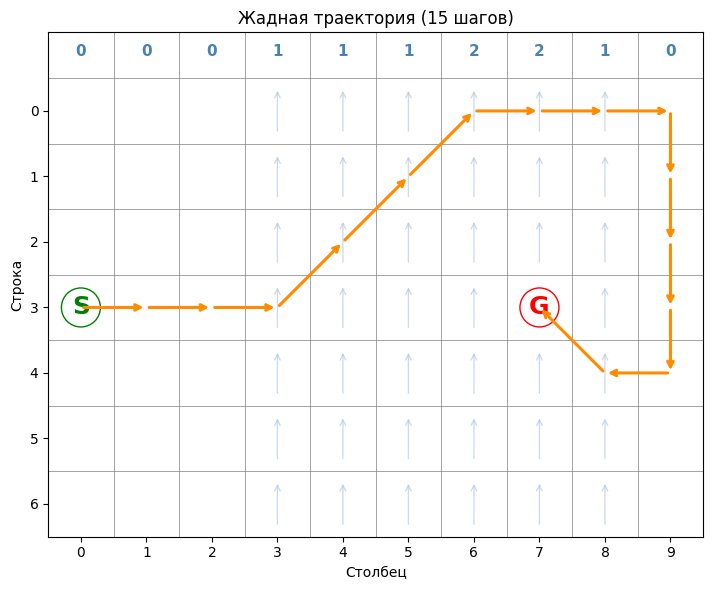
\includegraphics[width=0.7\textwidth]{original_trajectory.png}
        \caption{Жадная траектория для исходной задачи (15 шагов).}
    \end{figure}

    \textbf{Ходы короля (8 действий).} Диагональные ходы позволяют эффективнее компенсировать снос ветра. Минимальная длина жадной траектории — 7 шагов.
    \begin{figure}[H]
        \centering
        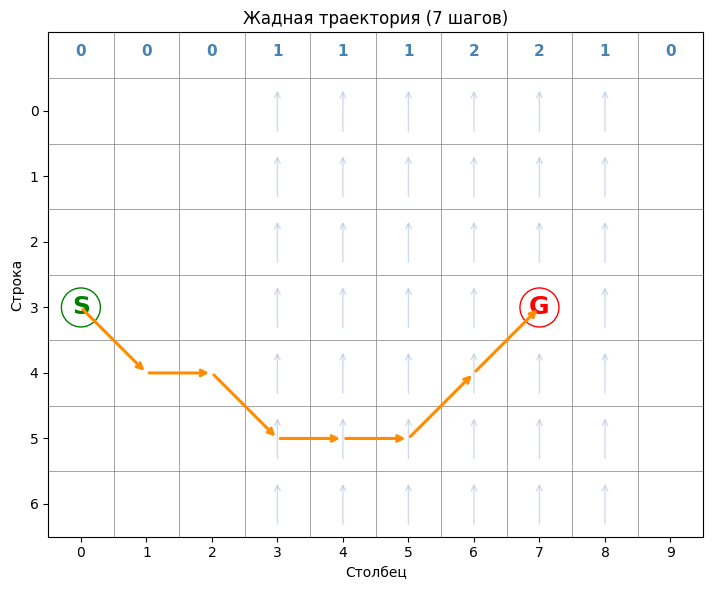
\includegraphics[width=0.7\textwidth]{diag_trajectory.png}
        \caption{Жадная траектория с ходами короля (7 шагов).}
    \end{figure}

    \textbf{Ходы короля + действие «стоять на месте» (9 действий).} Добавление девятого действия не улучшает результат: минимальная длина по-прежнему 7 шагов. Использовать ветер пассивно невыгодно, потому что бездействие тоже стоит $-1$ за шаг, а активное движение всегда даёт по крайней мере не худший прогресс.
    \begin{figure}[H]
        \centering
        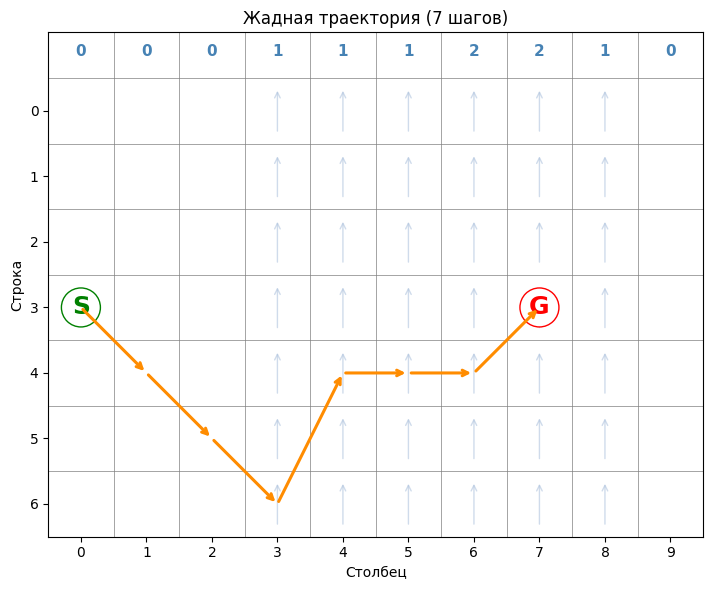
\includegraphics[width=0.7\textwidth]{diag_stay_trajectory.png}
        \caption{Жадная траектория с ходами короля и действием «стоять на месте» (7 шагов).}
    \end{figure}

    \textbf{Вывод.} Переход от 4 к 8 действиям сократил оптимальную длину эпизода более чем вдвое (с 15 до 7 шагов). Девятое действие не приносит дополнительного выигрыша.
\end{solution}
\notebook{06_09_10}{6.9}

\subsection{Упражнение 6.10. Стохастический ветер(c. 164)}
Решите задачу о ветреном сеточном мире с ходами короля в предположении, что воздействие ветра если и есть, то стохастическое: иногда оно отклоняется на 1 от средних значений, указанных под столбцом. Точнее, треть времени сила ветра средняя (как в предыдущем упражнении), ещё треть времени вас сдувает на дополнительную ячейку вверх, а ещё треть — на дополнительную ячейку вниз.
\begin{solution}
    \textbf{Код смотри в отдельном файле репозитория.} \\
    Алгоритм Sarsa с теми же параметрами: $\varepsilon = 0.1$, $\alpha = 0.5$, $Q(s, a) = 0$, 2000 эпизодов. Действия — ходы короля (8 направлений). Сила ветра в столбце с базовым значением $w$ применяется как $w - 1$, $w$ или $w + 1$ с равными вероятностями $1/3$.

    \begin{figure}[H]
        \centering
        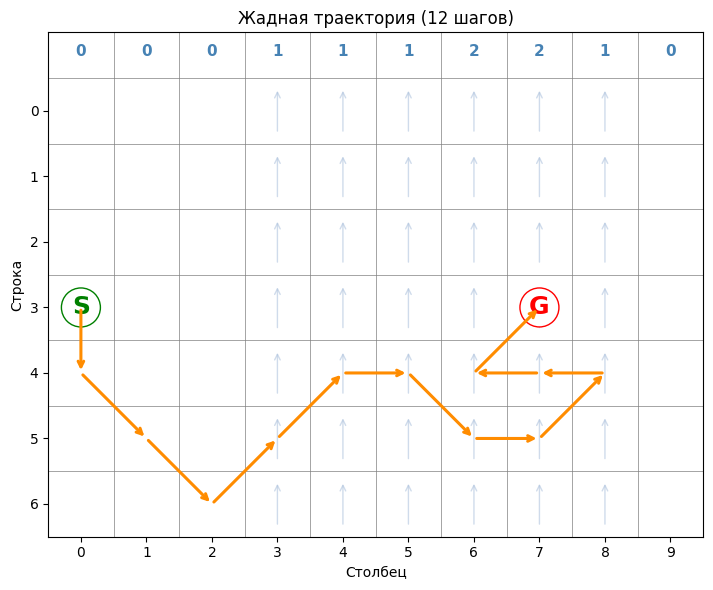
\includegraphics[width=0.7\textwidth]{6_10_trajectory.png}
        \caption{Одна из жадных траекторий при стохастическом ветре (12 шагов).}
    \end{figure}

    Из-за случайности ветра жадная траектория уже не детерминирована — каждый прогон даёт свою длину. По 100 прогонам жадной стратегии средняя длина эпизода составила $16.4 \pm 9.1$ шагов, с отдельными удачными прогонами в 12 шагов.

    \textbf{Вывод.} По сравнению с детерминированным случаем (7 шагов) стохастический ветер существенно усложняет задачу: оптимальная стратегия не может полагаться на точное знание сноса, и средняя длина эпизода более чем удваивается. Высокое стандартное отклонение отражает естественный разброс траекторий из-за случайности среды.
\end{solution}
\notebook{06_09_10}{6.10}

\subsection{Упражнение 6.11(c. 167)}
Почему Q-обучение считается методом управления с разделённой стратегией?
\begin{solution}
    В Q-обучении поведенческая и целевая политики различаются:
    \begin{itemize}
        \item \textbf{Поведенческая политика} (по ней выбираются действия в среде) — $\varepsilon$-жадная по $Q$, чтобы обеспечить покрытие;
        \item \textbf{Целевая политика} (та, чью функцию ценности мы оцениваем) — жадная по $Q$.
    \end{itemize}
    Это видно из самого правила обновления:
    \[
    Q(S, A) \leftarrow Q(S, A) + \alpha\Bigl[R + \gamma \max_{a'} Q(S', a') - Q(S, A)\Bigr].
    \]
    В качестве оценки следующего шага берётся $\max_{a'} Q(S', a')$ — ценность \emph{жадного} действия, а не реально выбранного $A'$ из $\varepsilon$-жадной политики. 
\end{solution}

\subsection{Упражнение 6.12(c. 167)}
Предположим, что выбор действия жадный. Будет ли тогда алгоритм Q-обучения в точности совпадать с Sarsa? Будут ли они выбирать в точности одинаковые действия и одинаково обновлять веса?
\begin{solution}
    \textbf{Обновления весов совпадают.} В Sarsa используется $Q(S', A')$, в Q-обучении — $\max_{a'} Q(S', a')$. Если $A'$ выбирается жадно, то $A' \in \arg\max_{a'} Q(S', a')$, и значит
    \[
    Q(S', A') = \max_{a'} Q(S', a').
    \]
    Поэтому при жадном выборе действий правила обновления тождественны по значению, независимо от того, как разрешаются ничьи.

    \textbf{Последовательности действий могут различаться.} В состояниях, где у нескольких действий одинаковое $Q$, жадный выбор разрешает ничью случайно. Если в двух алгоритмах ничьи разрешаются независимыми случайными механизмами, то выбранные действия могут отличаться. При фиксированном детерминированном правиле разрешения ничьих (одинаковом для обоих алгоритмов) последовательности действий совпадают.

    \textbf{Итог.} При жадном выборе действий обновления весов всегда идентичны. Последовательности действий идентичны при условии одинакового разрешения ничьих.
\end{solution}

\subsection{*Упражнение 6.13(c. 171)}
Как выглядят уравнения обновления для двойной версии алгоритма Expected Sarsa с $\varepsilon$-жадной целевой стратегией?
\begin{solution}
    Поддерживаем две независимые оценки $Q_1$ и $Q_2$. На каждом шаге с вероятностью $0.5$ обновляем одну из них, с вероятностью $0.5$ — другую. Политика, по которой берётся ожидание, строится из той же оценки, которую обновляем; ценности под суммой берутся из другой оценки. Это разделяет роли «выбор» и «оценка» и устраняет смещение максимизации.

    Обозначим $\varepsilon$-жадную политику относительно оценки $Q_i$ как
    \[
    \pi_i(a \mid s) =
    \begin{cases}
        1 - \varepsilon + \dfrac{\varepsilon}{|\mathcal{A}(s)|}, & \text{если } a = \arg\max_{a'} Q_i(s, a'), \\[6pt]
        \dfrac{\varepsilon}{|\mathcal{A}(s)|}, & \text{иначе}.
    \end{cases}
    \]

    Тогда правила обновления:
    \begin{itemize}
        \item С вероятностью $0.5$:
        \[
        Q_1(S, A) \leftarrow Q_1(S, A) + \alpha\Bigl[R + \gamma \sum_{a'} \pi_1(a' \mid S') \, Q_2(S', a') - Q_1(S, A)\Bigr].
        \]
        \item Иначе:
        \[
        Q_2(S, A) \leftarrow Q_2(S, A) + \alpha\Bigl[R + \gamma \sum_{a'} \pi_2(a' \mid S') \, Q_1(S', a') - Q_2(S, A)\Bigr].
        \]
    \end{itemize}
\end{solution}

\subsection{Упражнение 6.14(c. 173)}
Опишите, как можно переформулировать задачу Джека об аренде машин (пример 4.2) в терминах послесостояний. Почему в этой конкретной задаче такая постановка, скорее всего, приведёт к ускорению сходимости?
\begin{solution}
    \textbf{Послесостояние в задаче Джека.} Послесостояние — это конфигурация офисов сразу после ночного перегона машин, но до дневных запросов и возвратов. Если утром в офисах было $(s_1, s_2)$ и Джек перегнал $a$ машин, послесостояние равно $\sigma(s, a) = (s_1 - a, s_2 + a)$.

    \textbf{Почему это ускоряет сходимость.} Многие пары $(s, a)$ приводят к одному и тому же послесостоянию. Например, послесостояние $(8, 7)$ достигается из $(10, 5)$ при $a = -2$, из $(9, 6)$ при $a = -1$, из $(8, 7)$ при $a = 0$ и т.\,д. Дальнейшая динамика для всех этих пар идентична, поэтому различать их бессмысленно.

    В обычной формулировке через $q(s, a)$ алгоритм отдельно учит ценность каждой такой пары, разбивая статистику между ними. В формулировке через $v(\sigma)$ все эти пары обновляют одну общую оценку, что даёт:
    \begin{itemize}
        \item меньше обучаемых параметров (пространство послесостояний значительно меньше пространства пар $(s, a)$);
        \item больше данных на параметр — любой опыт из любой пары вносит вклад в одну и ту же оценку.
    \end{itemize}
    Оба эффекта ускоряют сходимость по сравнению со стандартной формулировкой.
\end{solution}

\section{Глава 7. n-шаговый бутстрэппинг}
\subsection{Упражнение 7.1(c. 179)}
В главе 6 мы отметили, что ошибку Монте-Карло можно записать в виде суммы TD-ошибок (6.6), если оценка ценности не изменяется от шага к шагу. Покажите, что $n$-шаговую ошибку в формуле (7.2) также можно записать в виде суммы TD-ошибок (опять-таки, если оценки ценности не изменяются), что обобщает ранее полученный результат.
\begin{equation}
    G_t - V(S_t) = \sum_{k=t}^{T-1} \gamma^{k-t} \delta_k.
    \tag{6.6}
\end{equation}
\begin{equation}
    V_{t+n}(S_t) \doteq V_{t+n-1}(S_t) + \alpha\left[G_{t:t+n} - V_{t+n-1}(S_t)\right], \quad 0 \le t < T.
    \tag{7.2}
\end{equation}
\begin{solution}
    $n$-шаговая ошибка в (7.2) --- это величина $G_{t:t+n} - V_{t+n-1}(S_t)$. По условию ценности не изменяются от шага к шагу, поэтому индекс времени у $V$ можно опустить: $V_{t+n-1}(S_t) = V(S_t)$. Нужно показать, что эта ошибка равна сумме $n$ подряд идущих TD-ошибок.

    Распишем $n$-шаговый доход через первое вознаграждение и оставшийся доход. Из определения (7.1) следует
    \[
    G_{t:t+n} = R_{t+1} + \gamma G_{t+1:t+n}.
    \]
    Это верно при $n \ge 1$. Здесь мы пользуемся тем, что усечённый доход с горизонтом $n$ шагов от момента $t$ --- это первое вознаграждение плюс усечённый доход с горизонтом $n-1$ шагов от момента $t+1$.

    Теперь действуем так же, как в выводе (6.6). Прибавим и вычтем $\gamma V(S_{t+1})$:
    \begin{align*}
        G_{t:t+n} - V(S_t) &= R_{t+1} + \gamma G_{t+1:t+n} - V(S_t) + \gamma V(S_{t+1}) - \gamma V(S_{t+1}) \\
        &= \bigl(R_{t+1} + \gamma V(S_{t+1}) - V(S_t)\bigr) + \gamma\bigl(G_{t+1:t+n} - V(S_{t+1})\bigr) \\
        &= \delta_t + \gamma\bigl(G_{t+1:t+n} - V(S_{t+1})\bigr).
    \end{align*}
    В скобке снова стоит $n$-шаговая ошибка, но уже для момента $t+1$ и с горизонтом на единицу меньше. Применим к ней то же самое разложение:
    \begin{align*}
        G_{t:t+n} - V(S_t) &= \delta_t + \gamma\bigl(G_{t+1:t+n} - V(S_{t+1})\bigr) \\
        &= \delta_t + \gamma \delta_{t+1} + \gamma^2 \bigl(G_{t+2:t+n} - V(S_{t+2})\bigr) \\
        &= \delta_t + \gamma \delta_{t+1} + \gamma^2 \delta_{t+2} + \dots + \gamma^{n-1}\bigl(G_{t+n:t+n} - V(S_{t+n})\bigr).
    \end{align*}
    Раскладывание останавливается, когда горизонт усечения становится нулевым. По определению $n$-шагового дохода $G_{t+n:t+n} = V(S_{t+n})$ (доход с нулевым числом шагов --- это просто оценка ценности). Поэтому последнее слагаемое обнуляется:
    \[
    \gamma^{n-1}\bigl(G_{t+n:t+n} - V(S_{t+n})\bigr) = \gamma^{n-1}\bigl(V(S_{t+n}) - V(S_{t+n})\bigr) = 0.
    \]
    В итоге получаем
    \[
    G_{t:t+n} - V(S_t) = \sum_{k=t}^{t+n-1} \gamma^{k-t} \delta_k.
    \]
    Это сумма $n$ подряд идущих TD-ошибок, что и требовалось.

    Замечание: при $n = T - t$ доход $G_{t:t+n}$ становится обыкновенным полным доходом $G_t$, верхний предел суммы превращается в $T-1$, и формула переходит в (6.6). Так что результат главы 6 --- это частный случай при $n \to T-t$.
\end{solution}

\subsection{Упражнение 7.2(c. 179)}
В случае $n$-шагового метода оценки ценности изменяются от шага к шагу,
поэтому алгоритм, в котором используется сумма TD-ошибок (см. предыдущее
упражнение) вместо ошибки в формуле (7.2), отличается от описанного выше.
Лучше он или хуже? Придумайте и запрограммируйте простой эксперимент,
чтобы ответить на этот вопрос эмпирически.
\begin{equation}
    V_{t+n}(S_t) \doteq V_{t+n-1}(S_t) + \alpha\left[G_{t:t+n} - V_{t+n-1}(S_t)\right],
    \quad 0 \le t < T.
    \tag{7.2}
\end{equation}
\begin{solution}
    В упражнении 7.1 равенство $G_{t:t+n}-V(S_t)=\sum_{k=t}^{t+n-1}\gamma^{k-t}\delta_k$
    выполнено точно только если все $\delta_k$ посчитаны с одной и той же $V$.
    В классическом алгоритме (7.2) бутстрап-член $V(S_{\tau+n})$ всегда свежий.
    В варианте с суммой TD-ошибок каждая $\delta_k$ считается один раз и
    сохраняется, поэтому разные ошибки используют разные версии $V$ ---
    обновление работает с устаревшими оценками.

    \textbf{Эксперимент.} Сеточный мир $5\times5$, завышенная инициализация
    $V(s)=+5$, метрика --- RMSE до $v_\pi$ по эпизодам, усреднённая по прогонам,
    $n\in\{1,2,4,8,16\}$.

    \begin{figure}[ht]
        \centering
        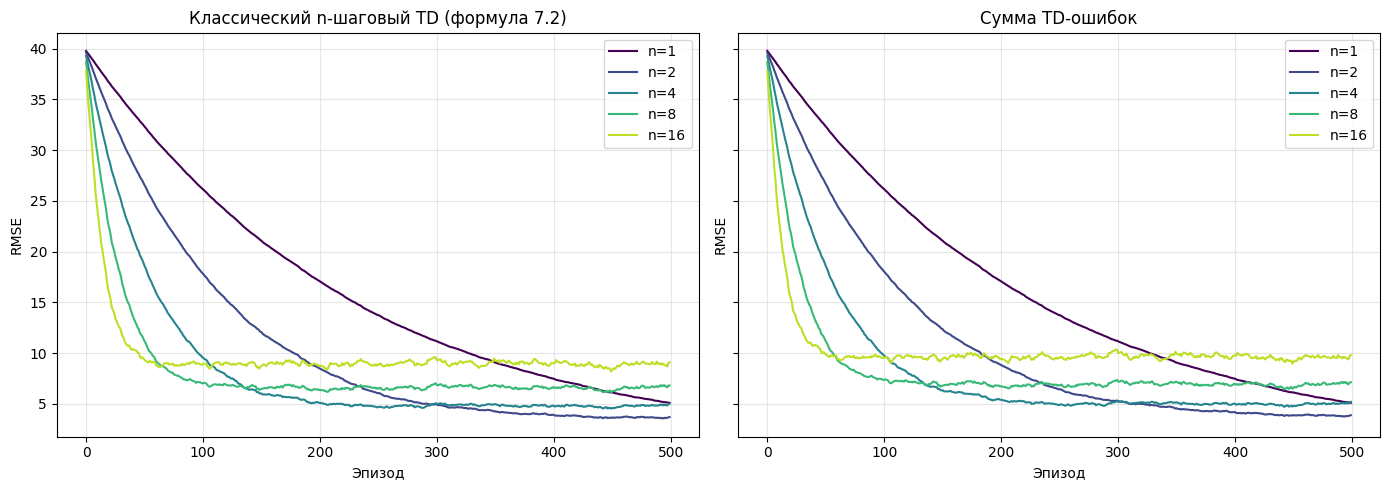
\includegraphics[width=\textwidth]{7_2_sol_rmse.png}
        \caption{RMSE классического алгоритма (7.2) и варианта с суммой TD-ошибок.}
    \end{figure}
    \begin{figure}[ht]
        \centering
        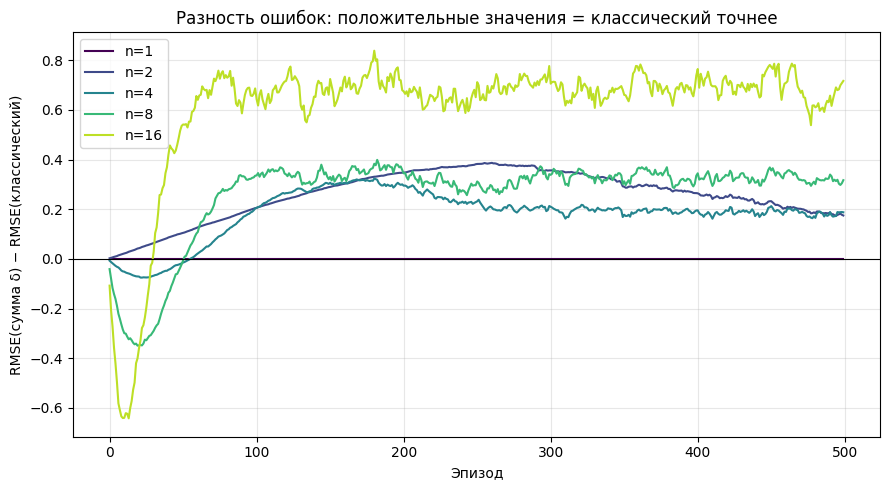
\includegraphics[width=0.7\textwidth]{7_2_sol.png}
        \caption{Разность RMSE: положительные значения --- классический точнее.}
    \end{figure}

    \textbf{Результаты.} При $n=1$ алгоритмы совпадают тождественно. В установившемся режиме разность положительна и растёт с $n$.
    В первые $\sim$30 эпизодов при больших $n$ разность уходит в минус: устаревшие
    ошибки тормозят резкий спад завышенной $V$, что временно ближе к истине.

    \textbf{Вывод.} Вариант с суммой сохранённых TD-ошибок \emph{хуже}: разница
    растёт с $n$ и исчезает при $n=1$. Причина --- использование устаревших оценок
    $V$; в коротком переходном режиме это может помогать, но в целом вредит.
\end{solution}
\notebook{07_02}{7.2}

\subsection{Упражнение 7.3(c. 181)}
Как вы думаете, почему в примерах из этой главы используется более масштабная задача о случайном блуждании (с 19, а не 5 состояниями)? Верно ли, что при меньшем блуждании более выгодным оказалось бы другое значение $n$? А что, если в большем блуждании изменить результат левой части с $0$ на $-1$? Повлияло бы это на выбор наилучшего значения?
\begin{solution}
    \textbf{Почему 19 состояний.} Цель рис. 7.2 --- показать, что лучше всего
    работают промежуточные $n$. Для этого нужно, чтобы крайние варианты были
    заметно хуже среднего. В короткой цепочке из 5 состояний эпизод слишком
    короткий: при $n$ больше длины эпизода $n$-шаговый доход превращается в
    полный доход, и все большие $n$ дают один и тот же метод Монте-Карло.
    Различимых значений $n$ остаётся мало, и выраженного минимума на кривой
    ошибки не получится. Длинная цепочка даёт достаточно места, чтобы развести
    методы по $n$ и увидеть U-образную кривую.
 
    \textbf{Другое $n$ для маленькой задачи.} Да. Оптимальное $n$ соразмерно
    длине эпизода. В цепочке из 5 состояний уже двух-трёх шагов хватает, чтобы
    обновление дошло до всех посещённых состояний, а большие $n$ схлопываются в
    Монте-Карло. Поэтому оптимум сместился бы к малым $n$ и стал бы менее
    выраженным.
 
    \textbf{Замена $0$ на $-1$ слева.} Да, повлияло бы. Выгода большого $n$ ---
    быстро доставлять коррекцию к удалённым состояниям; она велика там, где у
    этих состояний большая начальная ошибка. Замена награды меняет истинные
    ценности (диапазон $[0,1]$ переходит в $[-1,+1]$), а значит и профиль
    начальной ошибки $V_0 - v_\pi$ --- даже при одинаковой инициализации, так
    как $v_\pi$ у задач разные.
\end{solution}

\subsection{Упражнение 7.4(c. 183)}
Докажите, что $n$-шаговый доход в методе Sarsa (7.4) можно точно выразить
в терминах новой TD-ошибки:
\begin{multline}
    G_{t:t+n} = Q_{t-1}(S_t, A_t) \\
    + \sum_{k=t}^{\min(t+n,T)-1}
    \gamma^{k-t}\left[R_{k+1} + \gamma Q_k(S_{k+1}, A_{k+1}) - Q_{k-1}(S_k, A_k)\right].
    \tag{7.6}
\end{multline}
\begin{multline}
    G_{t:t+n} \doteq R_{t+1} + \gamma R_{t+2} + \dots + \gamma^{n-1} R_{t+n} \\
    + \gamma^n Q_{t+n-1}(S_{t+n}, A_{t+n}), \quad n \ge 1,\ 0 \le t < T-n.
    \tag{7.4}
\end{multline}
\begin{solution}
    Обозначим TD-ошибку для ценности действий
    \[
    \delta_k \doteq R_{k+1} + \gamma Q_k(S_{k+1}, A_{k+1}) - Q_{k-1}(S_k, A_k).
    \]
    Распишем сумму из правой части (7.6), считая для удобства $t+n \le T$
    (тогда верхний предел равен $t+n-1$):
    \begin{align*}
        \sum_{k=t}^{t+n-1} \gamma^{k-t} \delta_k
        &= \sum_{k=t}^{t+n-1} \gamma^{k-t} R_{k+1}
        + \sum_{k=t}^{t+n-1} \gamma^{k-t+1} Q_k(S_{k+1}, A_{k+1}) \\
        &\quad - \sum_{k=t}^{t+n-1} \gamma^{k-t} Q_{k-1}(S_k, A_k).
    \end{align*}
    В средней сумме сделаем замену индекса $j = k+1$, тогда она пробегает
    $j = t+1, \dots, t+n$:
    \[
    \sum_{k=t}^{t+n-1} \gamma^{k-t+1} Q_k(S_{k+1}, A_{k+1})
    = \sum_{j=t+1}^{t+n} \gamma^{j-t} Q_{j-1}(S_j, A_j).
    \]
    Это та же величина, что и последняя сумма, только с другими пределами.
    При вычитании совпадающие члены для $j = t+1, \dots, t+n-1$ сокращаются,
    остаются крайние:
    \[
    \begin{aligned}
    &\sum_{j=t+1}^{t+n} \gamma^{j-t} Q_{j-1}(S_j, A_j)
    - \sum_{k=t}^{t+n-1} \gamma^{k-t} Q_{k-1}(S_k, A_k) \\
    &\qquad = \gamma^n Q_{t+n-1}(S_{t+n}, A_{t+n}) - Q_{t-1}(S_t, A_t).
    \end{aligned}
    \]
    Подставляя обратно, получаем
    \[
    \sum_{k=t}^{t+n-1} \gamma^{k-t} \delta_k
    = \underbrace{\sum_{k=t}^{t+n-1} \gamma^{k-t} R_{k+1}
    + \gamma^n Q_{t+n-1}(S_{t+n}, A_{t+n})}_{=\ G_{t:t+n}\ \text{по (7.4)}}
    - Q_{t-1}(S_t, A_t).
    \]
    Первые два слагаемых --- это в точности определение $G_{t:t+n}$ из (7.4).
    Перенося $Q_{t-1}(S_t, A_t)$ влево, приходим к (7.6):
    \[
    G_{t:t+n} = Q_{t-1}(S_t, A_t) + \sum_{k=t}^{t+n-1} \gamma^{k-t} \delta_k.
    \]
    Если эпизод заканчивается раньше ($t+n > T$), доход обрывается на шаге $T$,
    и верхний предел суммы становится $\min(t+n,T)-1$ --- это и записано в (7.6).
\end{solution}

\subsection{Упражнение 7.5(c. 186)}
Напишите псевдокод описанного выше алгоритма предсказания ценности состояния
с разделённой стратегией.
\begin{solution}
    Алгоритм совпадает по структуре с $n$-шаговым TD-предсказанием, но
    $n$-шаговый доход вычисляется по рекуррентной формуле (7.13):
    \[
    G_{t:h} = \rho_t\bigl(R_{t+1} + \gamma G_{t+1:h}\bigr)
    + (1-\rho_t)V_{h-1}(S_t), \qquad \rho_t = \frac{\pi(A_t|S_t)}{b(A_t|S_t)},
    \]
    с базой $G_{h:h} = V_{h-1}(S_h)$. Рекурсия разворачивается в один цикл,
    идущий от $h$ к $\tau$: переменная $G$ инициализируется базой и на каждом
    шаге пересчитывается. Дополнительной памяти не требуется --- значения
    $\rho_k$, $R_{k+1}$, $S_k$ алгоритм уже хранит.

    \begin{algorithm}[H]
        \DontPrintSemicolon
        \KwIn{поведенческая стратегия $b$ такая, что $b(a|s) > 0$ для всех
        $s \in \mathcal{S},\ a \in \mathcal{A}$; целевая стратегия $\pi$}
        Параметры: размер шага $\alpha \in (0,1]$, целое $n > 0$\;
        Инициализировать $V(s)$ произвольно для всех $s \in \mathcal{S}$\;
        Все операции с $S_t$ и $R_t$ берут индекс по модулю $n+1$\;
        \BlankLine
        \ForEach{эпизод}{
            Инициализировать и сохранить $S_0 \ne$ заключительное состояние\;
            $T \leftarrow \infty$\;
            \For{$t = 0, 1, 2, \dots$}{
                \If{$t < T$}{
                    Выбрать действие $A_t \sim b(\cdot|S_t)$\;
                    Предпринять $A_t$, наблюдать и сохранить $R_{t+1}$, $S_{t+1}$\;
                    \If{$S_{t+1}$ --- заключительное состояние}{
                        $T \leftarrow t+1$\;
                    }
                }
                $\tau \leftarrow t - n + 1$ \tcp*{момент обновления}
                \If{$\tau \ge 0$}{
                    $h \leftarrow \min(\tau+n,\, T)$\;
                    $G \leftarrow V(S_h)$ \tcp*{база $G_{h:h}$}
                    \For{$k = h-1, h-2, \dots, \tau$}{
                        $\rho \leftarrow \dfrac{\pi(A_k|S_k)}{b(A_k|S_k)}$\;
                        $G \leftarrow \rho\,(R_{k+1} + \gamma G)
                        + (1-\rho)\,V(S_k)$\;
                    }
                    $V(S_\tau) \leftarrow V(S_\tau)
                    + \alpha\,[\,G - V(S_\tau)\,]$\;
                }
                \If{$\tau = T - 1$}{
                    \textbf{выйти из цикла}\;
                }
            }
        }
        \caption{$n$-шаговое предсказание $V \approx v_\pi$ с разделённой
        стратегией и переменным управлением}
    \end{algorithm}
\end{solution}

\subsection{Упражнение 7.6(c. 187)}
Докажите, что переменное управление в приведённых выше уравнениях не изменяет
математического ожидания дохода.
\begin{solution}
    Докажем для ценностей действий (формула 7.14); для ценностей состояний
    (7.13) рассуждение аналогично. Переменное управление --- это член,
    добавленный к доходу:
    \[
    C = \gamma\bar V_{h-1}(S_{t+1}) - \gamma\rho_{t+1}Q_{h-1}(S_{t+1}, A_{t+1}),
    \qquad \rho_{t+1} = \frac{\pi(A_{t+1}|S_{t+1})}{b(A_{t+1}|S_{t+1})}.
    \]
    Достаточно показать, что $\mathbb{E}_b[C] = 0$ --- тогда добавление $C$ не
    меняет математического ожидания дохода.

    Зафиксируем $S_{t+1} = s$ и возьмём условное математическое ожидание по
    выбору $A_{t+1} \sim b(\cdot|s)$. Первый член от $A_{t+1}$ не зависит и
    выходит из-под ожидания как есть. Второй член распишем суммой по действиям:
    \[
    \begin{aligned}
    \mathbb{E}_b\bigl[\rho_{t+1}Q_{h-1}(s, A_{t+1}) \mid s\bigr]
    &= \sum_a b(a|s)\,\frac{\pi(a|s)}{b(a|s)}\,Q_{h-1}(s, a) \\
    &= \sum_a \pi(a|s)\,Q_{h-1}(s, a).
    \end{aligned}
    \]
    Здесь $b(a|s)$ сократилось. По определению (7.8) ожидаемая ценность состояния
    есть усреднение $Q$ по целевой стратегии:
    \[
    \bar V_{h-1}(s) = \sum_a \pi(a|s)\,Q_{h-1}(s, a).
    \]
    Значит оба члена $C$ равны $\gamma\bar V_{h-1}(s)$, и
    \[
    \mathbb{E}_b[C \mid s]
    = \gamma\bar V_{h-1}(s) - \gamma\bar V_{h-1}(s) = 0
    \quad \text{при любом } s.
    \]
    По формуле полного математического ожидания $\mathbb{E}_b[C] = 0$.

    \textbf{Случай ценностей состояний (7.13).} Управляющий член ---
    $V_{h-1}(S_t) - \rho_t V_{h-1}(S_t)$. Оценка $V_{h-1}(S_t)$ от действия не
    зависит, поэтому, используя известный факт $\mathbb{E}_b[\rho_t \mid s] = 1$,
    \[
    \mathbb{E}_b\bigl[V_{h-1}(s) - \rho_t V_{h-1}(s) \mid s\bigr]
    = V_{h-1}(s)\bigl(1 - \mathbb{E}_b[\rho_t \mid s]\bigr)
    = V_{h-1}(s)(1 - 1) = 0.
    \]

    В обоих случаях работает одно и то же сокращение $b(a|s)\,\rho = \pi(a|s)$:
    для состояний оно сворачивается до $\mathbb{E}_b[\rho] = 1$, для действий ---
    до $\mathbb{E}_b[\rho Q] = \bar V$. Управляющий член при этом не константа:
    он коррелирует с доходом и снижает дисперсию, не внося смещения.
\end{solution}

\subsection{*Упражнение 7.7(c. 192)}
Напишите псевдокод описанного выше алгоритма предсказания ценности действий
с разделённой стратегией. Особое внимание обратите на условия завершения
рекурсии при достижении горизонта или конца эпизода.
\begin{solution}
    Алгоритм совпадает по структуре с $n$-шаговым предсказанием, но
    $n$-шаговый доход вычисляется по рекуррентной формуле (7.14):
    \[
    G_{t:h} = R_{t+1} + \gamma\rho_{t+1}\bigl(G_{t+1:h} - Q_{h-1}(S_{t+1}, A_{t+1})\bigr)
    + \gamma\bar V_{h-1}(S_{t+1}),
    \]
    где $\rho_{t+1} = \pi(A_{t+1}|S_{t+1})/b(A_{t+1}|S_{t+1})$ и
    $\bar V(s) = \sum_a \pi(a|s)Q(s,a)$. Рекурсия разворачивается в один цикл
    от $h$ к $\tau$. Условие завершения зависит от того, оборвался эпизод или
    нет:
    \begin{itemize}
        \item если $h \le T$ (горизонт внутри эпизода), база --- $G_{h:h} = Q(S_h, A_h)$;
        \item если $h > T$ (эпизод закончился раньше), база --- $G_{T-1:h} = R_T$.
    \end{itemize}

    \begin{algorithm}[H]
        \small
        \DontPrintSemicolon
        \KwIn{поведенческая стратегия $b$ с $b(a|s) > 0$ для всех $s, a$;
        целевая стратегия $\pi$}
        Параметры: размер шага $\alpha \in (0,1]$, целое $n > 0$\;
        Инициализировать $Q(s,a)$ произвольно для всех $s \in \mathcal{S},\ a \in \mathcal{A}$\;
        Все операции с $S_t$, $A_t$, $R_t$ берут индекс по модулю $n+1$\;
        \BlankLine
        \ForEach{эпизод}{
            Инициализировать $S_0 \ne$ заключительное состояние\;
            Выбрать действие $A_0 \sim b(\cdot|S_0)$\;
            $T \leftarrow \infty$\;
            \For{$t = 0, 1, 2, \dots$}{
                \If{$t < T$}{
                    Предпринять $A_t$, наблюдать и сохранить $R_{t+1}$, $S_{t+1}$\;
                    \eIf{$S_{t+1}$ --- заключительное состояние}{
                        $T \leftarrow t+1$\;
                    }{
                        Выбрать и сохранить $A_{t+1} \sim b(\cdot|S_{t+1})$\;
                    }
                }
                $\tau \leftarrow t - n + 1$ \tcp*{момент обновления}
                \If{$\tau \ge 0$}{
                    $h \leftarrow \tau + n$ \tcp*{горизонт}
                    \BlankLine
                    \tcc{База рекурсии — два случая}
                    \eIf{$h \ge T$}{
                        $G \leftarrow R_T$ \tcp*{эпизод закончился: $G_{T-1:h}=R_T$}
                        $k_{\text{start}} \leftarrow T - 2$\;
                    }{
                        $G \leftarrow Q(S_h, A_h)$ \tcp*{горизонт внутри: $G_{h:h}=Q(S_h,A_h)$}
                        $k_{\text{start}} \leftarrow h - 1$\;
                    }
                    \BlankLine
                    \tcc{Разворачиваем рекурсию (7.14) от $k_{\text{start}}$ к $\tau$}
                    \For{$k = k_{\text{start}},\ k_{\text{start}}-1,\ \dots,\ \tau$}{
                        $\rho \leftarrow \dfrac{\pi(A_{k+1}|S_{k+1})}{b(A_{k+1}|S_{k+1})}$\;
                        $\bar V \leftarrow \sum_a \pi(a|S_{k+1})\,Q(S_{k+1}, a)$\;
                        $G \leftarrow R_{k+1}
                        + \gamma\rho\,\bigl(G - Q(S_{k+1}, A_{k+1})\bigr)
                        + \gamma\bar V$\;
                    }
                    $Q(S_\tau, A_\tau) \leftarrow Q(S_\tau, A_\tau)
                    + \alpha\,[\,G - Q(S_\tau, A_\tau)\,]$\;
                }
            }
            \If{$\tau = T - 1$}{
                \textbf{выйти из цикла}\;
            }
        }
        \caption{$n$-шаговое предсказание $Q \approx q_\pi$ с разделённой
        стратегией и переменным управлением}
    \end{algorithm}

    \textbf{Пояснение к условиям завершения.} Если горизонт $h$ не достигнут
    раньше конца эпизода ($h < T$), доход обрывается на оценке $Q(S_h, A_h)$ и
    цикл идёт от $h-1$. Если же эпизод закончился до горизонта ($h \ge T$),
    последнего действия $A_h$ просто не существует, поэтому базой служит
    последнее реальное вознаграждение $R_T$, а цикл начинается с $T-2$. В обоих
    случаях рекурсия сворачивается в один проход без отдельной рекурсивной
    функции.
\end{solution}

\subsection{Упражнение 7.8(c. 187)}
Покажите, что общий (с разделённой стратегией) вариант $n$-шагового дохода
(7.13) всё ещё можно точно и компактно записать в виде суммы основанных
на состояниях TD-ошибок (6.5), если приближённая функция ценности состояний
не изменяется.
\begin{equation}
    G_{t:h} \doteq \rho_t\left(R_{t+1} + \gamma G_{t+1:h}\right) + (1-\rho_t)V(S_t),
    \quad t < h < T.
    \tag{7.13}
\end{equation}
\begin{equation}
    \delta_t \doteq R_{t+1} + \gamma V(S_{t+1}) - V(S_t).
    \tag{6.5}
\end{equation}
\begin{solution}
    Раз $V$ не меняется, пишем её без индексов. Вынесем $V(S_t)$ из (7.13) и
    вставим в скобку $\gamma V(S_{t+1})$, чтобы выделить $\delta_t$:
    \begin{align*}
        G_{t:h} &= V(S_t) + \rho_t\left(R_{t+1} + \gamma G_{t+1:h} - V(S_t)\right)\\
                &= V(S_t) + \rho_t\left(\delta_t + \gamma\left(G_{t+1:h} - V(S_{t+1})\right)\right).
    \end{align*}

    Обозначим $E_t \doteq G_{t:h} - V(S_t)$. Тогда $E_t = \rho_t(\delta_t + \gamma E_{t+1})$,
    причём из условия завершения $G_{h:h} = V(S_h)$ следует $E_h = 0$. Раскручивая
    рекурсию вниз:
    \begin{equation*}
        E_t = \sum_{k=t}^{h-1} \gamma^{k-t}\left(\prod_{i=t}^{k}\rho_i\right)\delta_k,
    \end{equation*}
    откуда
    \begin{equation}
        G_{t:h} = V(S_t) + \sum_{k=t}^{h-1}
        \gamma^{k-t}\left(\prod_{i=t}^{k}\rho_i\right)\delta_k.
        \tag{$\ast$}
    \end{equation}

    Проверим края: при всех $\rho_i = 1$ получаем формулу (6.6), а при $\rho_t = 0$
    --- $G_{t:h} = V(S_t)$, что совпадает с (7.13). Равенство ($\ast$) точное только
    потому, что $V$ неизменна: иначе члены $\gamma V(S_{t+1})$ на соседних шагах
    брались бы из разных версий $V$ и не сокращались бы.
\end{solution}

\subsection{Упражнение 7.9(c. 187)}
Повторите предыдущее упражнение для варианта $n$-шагового дохода с разделённой
стратегией для ценностей действий (7.14) и TD-ошибки в смысле Expected Sarsa
(величина в квадратных скобках в формуле (6.9)).
\begin{equation}
    G_{t:h} \doteq R_{t+1} + \gamma\left(\rho_{t+1}\left(G_{t+1:h} - Q(S_{t+1}, A_{t+1})\right)
    + \bar{V}(S_{t+1})\right), \quad t < h \le T.
    \tag{7.14}
\end{equation}
\begin{equation}
    \delta_t \doteq R_{t+1} + \gamma\bar{V}(S_{t+1}) - Q(S_t, A_t),
    \qquad \bar{V}(s) \doteq \sum_a \pi(a\,|\,s)\,Q(s, a).
    \tag{6.9}
\end{equation}
\begin{solution}
    Раз $Q$ не меняется, пишем её без индексов. В (7.14) первое действие не
    взвешивается по значимости, поэтому рекурсия здесь по $Q$, а не по $V$.
    Вынесем $Q(S_t, A_t)$ и подставим $\gamma\bar V(S_{t+1})$, чтобы выделить $\delta_t$:
    \begin{align*}
        G_{t:h}
        &= Q(S_t, A_t)
        + \underbrace{R_{t+1} + \gamma\bar V(S_{t+1}) - Q(S_t, A_t)}_{\delta_t}\\
        &\quad + \gamma\rho_{t+1}\left(G_{t+1:h} - Q(S_{t+1}, A_{t+1})\right)\\
        &= Q(S_t, A_t) + \delta_t
        + \gamma\rho_{t+1}\left(G_{t+1:h} - Q(S_{t+1}, A_{t+1})\right).
    \end{align*}

    Обозначим $E_t \doteq G_{t:h} - Q(S_t, A_t)$. Тогда $E_t = \delta_t + \gamma\rho_{t+1}E_{t+1}$,
    причём из условия завершения рекурсии $E_h = 0$. Обрати внимание: первый член
    $\delta_t$ идёт без коэффициента $\rho$, а дальше каждый следующий уровень
    домножается на $\rho_{t+1}, \rho_{t+2}, \dots$. Раскручивая:
    \begin{equation*}
        E_t = \sum_{k=t}^{h-1} \gamma^{k-t}\left(\prod_{i=t+1}^{k}\rho_i\right)\delta_k,
    \end{equation*}
    где при $k=t$ пустое произведение равно $1$. Отсюда
    \begin{equation}
        G_{t:h} = Q(S_t, A_t) + \sum_{k=t}^{h-1}
        \gamma^{k-t}\left(\prod_{i=t+1}^{k}\rho_i\right)\delta_k.
        \tag{$\ast$}
    \end{equation}

    Отличие от упражнения 7.8 в том, что произведение коэффициентов начинается с
    $i=t+1$: первое действие $A_t$ уже выбрано и в выборку по значимости не входит.
    Как и там, равенство ($\ast$) точное лишь потому, что $Q$ неизменна --- иначе
    члены $\gamma\bar V(S_{t+1})$ на соседних шагах брались бы из разных версий $Q$
    и не сокращались бы.
\end{solution}

\subsection{Упражнение 7.10(c. 187)}
Придумайте не очень сложную задачу предсказания
с разделённой стратегией и воспользуйтесь ей, чтобы показать, что алгоритм
обучения с разделённой стратегией, в котором используются уравнения (7.13) и
(7.2), эффективнее более простого алгоритма, в котором используются уравнения
(7.1) и (7.9).
\begin{equation}
    \begin{aligned}
    G_{t:t+n} \doteq{}& R_{t+1} + \gamma R_{t+2} + \cdots
    + \gamma^{n-1}R_{t+n} \\
    &+ \gamma^n V_{t+n-1}(S_{t+n}), \quad n \ge 1,\ 0 \le t < T-n.
    \end{aligned}
    \tag{7.1}
\end{equation}
\begin{equation}
    V_{t+n}(S_t) \doteq V_{t+n-1}(S_t) + \alpha\left[G_{t:t+n} - V_{t+n-1}(S_t)\right],
    \quad 0 \le t < T.
    \tag{7.2}
\end{equation}
\begin{equation}
    V_{t+n}(S_t) \doteq V_{t+n-1}(S_t)
    + \alpha\rho_{t:t+n-1}\left[G_{t:t+n} - V_{t+n-1}(S_t)\right],
    \quad 0 \le t < T.
    \tag{7.9}
\end{equation}
\begin{equation}
    G_{t:h} \doteq \rho_t\left(R_{t+1} + \gamma G_{t+1:h}\right) + (1-\rho_t)V_{h-1}(S_t),
    \quad t < h < T.
    \tag{7.13}
\end{equation}
\begin{solution}
    \textbf{Код смотри в отдельном файле репозитория.}
    \textbf{Задача.} Случайное блуждание на 19 состояниях (пример 7.1), награда
    $+1$ справа и $-1$ слева. Поведенческая стратегия $b$ равновероятная;
    целевая $\pi$ задаётся одним числом $\pi(\text{вправо}\,|\,s)=p$ во всех
    состояниях, так что $\rho$ на шаге равен $p/0{,}5$ для хода вправо и
    $(1-p)/0{,}5$ для хода влево. Берём $n=4$ и $p\in\{0{,}1;\,0{,}3;\,0{,}5\}$.
    Истинные $v_\pi$ для каждого $p$ считаются точно из уравнений Беллмана,
    метрика --- RMSE до $v_\pi$ по состояниям и эпизодам, усреднённый по 100
    прогонам. При $p=0{,}5$ задача on-policy, поэтому оба метода обязаны совпасть
    (это проверка кода; при $n=1$ они совпадают тождественно).

    \begin{figure}[ht]
        \centering
        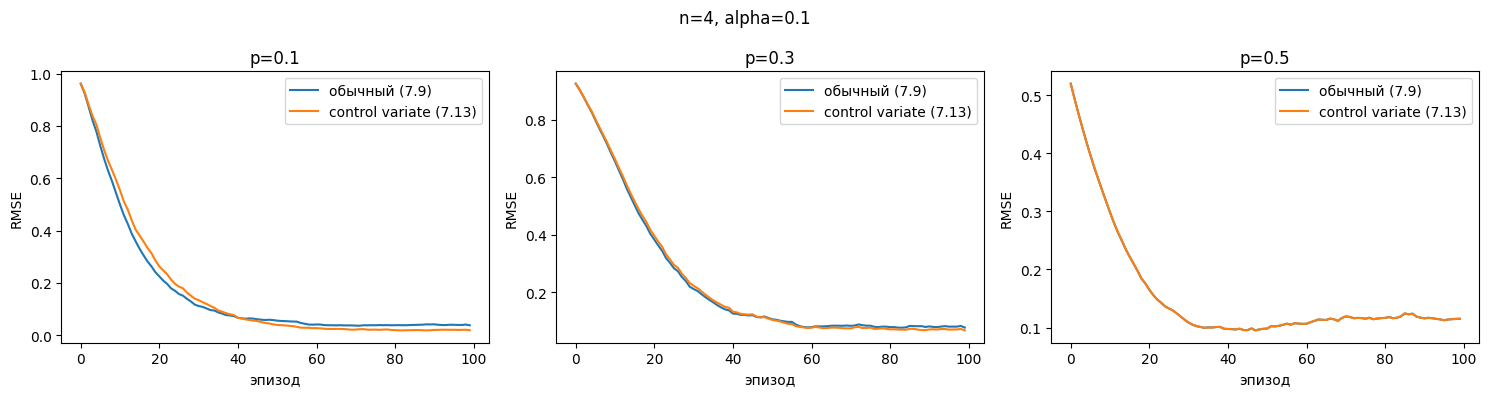
\includegraphics[width=\textwidth]{alpha_0_1.png}
        \caption{$n=4$, $\alpha=0{,}1$: при малом шаге методы почти неотличимы.}
    \end{figure}
    \begin{figure}[ht]
        \centering
        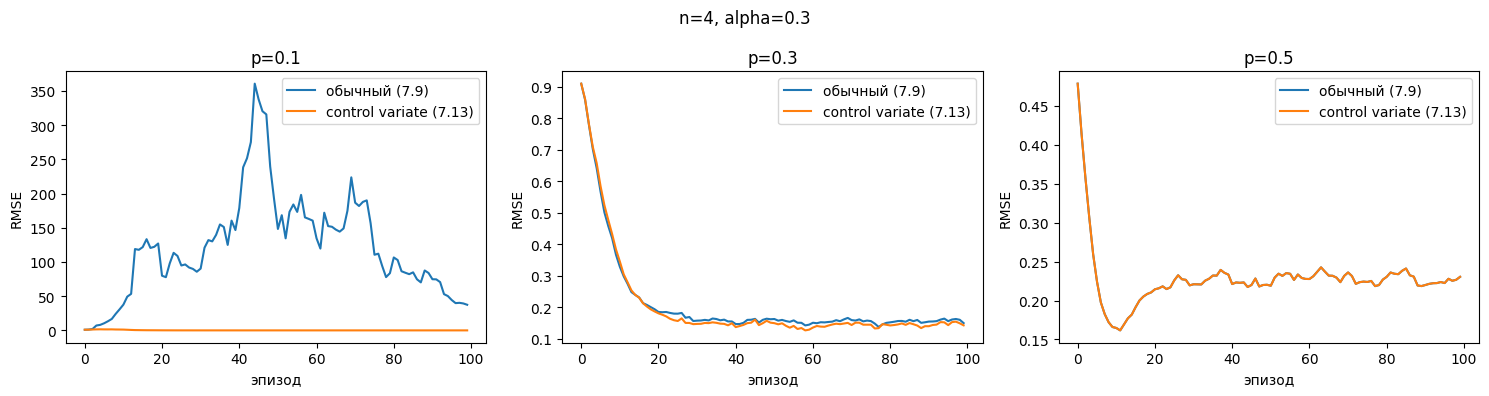
\includegraphics[width=\textwidth]{alpha_0_3.png}
        \caption{$n=4$, $\alpha=0{,}3$: при $p=0{,}1$ обычный метод (7.9)
        разваливается, control variate остаётся устойчивым (выглядит как ноль
        из-за масштаба оси).}
    \end{figure}
    \begin{figure}[H]
        \centering
        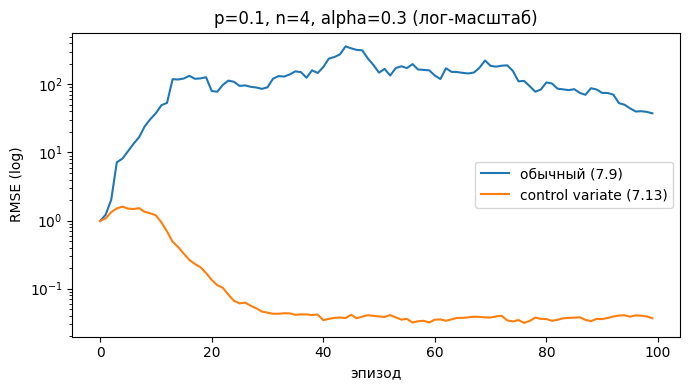
\includegraphics[width=0.7\textwidth]{log_alpha_0_3.png}
        \caption{Тот же случай $p=0{,}1$ в лог-масштабе: обе кривые видны
        раздельно, control variate точнее обычного на два порядка.}
    \end{figure}

    \textbf{Результаты.} При $p=0{,}5$ кривые совпадают --- веса равны 1. С ростом
    смещения $\pi$ коэффициенты $\rho$ всё сильнее отличаются от 1, и на окне
    $n=4$ их произведения разлетаются в широком диапазоне. При малом шаге
    $\alpha=0{,}1$ это почти незаметно. При $\alpha=0{,}3$ и сильном off-policy
    $p=0{,}1$ обычный метод (7.9) умножает обновление на огромные произведения
    $\rho$ и расходится (RMSE доходит до сотен), тогда как control variate
    усекает доход до текущей оценки $V$ в точках с малым $\rho$ и потому остаётся
    устойчивым.

    \textbf{Вывод.} Алгоритм с control variate (7.13)+(7.2) \emph{эффективнее}:
    при сильном расхождении $\pi$ и $b$ он точнее и не разваливается при больших
    шагах, а при $n=1$ и в on-policy случае совпадает с обычным.
\end{solution}
\notebook{07_10}{7.10}

\subsection{Упражнение 7.11(c. 187)}
Покажите, что если приближённые ценности действий не изменяются, то доход в
алгоритме обновления по дереву (7.16) можно записать в виде суммы основанных
на математическом ожидании TD-ошибок:
\begin{equation*}
    G_{t:t+n} = Q(S_t, A_t)
    + \sum_{k=t}^{\min(t+n,\,T-1)} \delta_k \prod_{i=t+1}^{k} \gamma\pi(A_i\,|\,S_i),
\end{equation*}
где $\delta_t \doteq R_{t+1} + \gamma\bar{V}_t(S_{t+1}) - Q(S_t, A_t)$, а $\bar V_t$
определено формулой (7.8).
\begin{equation}
    \begin{aligned}
    G_{t:t+n} \doteq{}& R_{t+1}
    + \gamma\sum_{a\ne A_{t+1}}\pi(a\,|\,S_{t+1})Q(S_{t+1},a)\\
    &+ \gamma\pi(A_{t+1}\,|\,S_{t+1})G_{t+1:t+n}, \quad t < T-1.
    \end{aligned}
    \tag{7.16}
\end{equation}
\begin{solution}
    Раз $Q$ не меняется, пишем её без индексов. Сумма по $a\ne A_{t+1}$ -- это
    полное $\bar V(S_{t+1})$ без члена выбранного действия:
    \begin{equation*}
        \sum_{a\ne A_{t+1}}\pi(a|S_{t+1})Q(S_{t+1},a)
        = \bar V(S_{t+1}) - \pi(A_{t+1}|S_{t+1})Q(S_{t+1},A_{t+1}).
    \end{equation*}
    Подставим это в (7.16) и сгруппируем слагаемые с $\gamma\pi(A_{t+1}|S_{t+1})$:
    \begin{align*}
        G_{t:t+n} &= \underbrace{R_{t+1} + \gamma\bar V(S_{t+1})}_{\delta_t + Q(S_t,A_t)}
                     + \gamma\pi(A_{t+1}|S_{t+1})\bigl(G_{t+1:t+n} - Q(S_{t+1},A_{t+1})\bigr)\\
                  &= Q(S_t,A_t) + \delta_t
                     + \gamma\pi(A_{t+1}|S_{t+1})\bigl(G_{t+1:t+n} - Q(S_{t+1},A_{t+1})\bigr).
    \end{align*}

    Обозначим $E_t \doteq G_{t:t+n} - Q(S_t, A_t)$. Тогда
    \begin{equation*}
        E_t = \delta_t + \gamma\pi(A_{t+1}|S_{t+1})\,E_{t+1}.
    \end{equation*}
    В отличие от упражнений 7.8--7.9 множитель при рекурсивном члене здесь не
    $\gamma\rho$, а $\gamma\pi(A_{t+1}|S_{t+1})$ -- это и даёт произведение
    $\prod\gamma\pi(A_i|S_i)$. Раскручивая рекурсию:
    \begin{equation*}
        E_t = \sum_{k=t}^{\min(t+n,\,T-1)} \delta_k \prod_{i=t+1}^{k}\gamma\pi(A_i|S_i),
    \end{equation*}
    где при $k=t$ произведение пустое и равно $1$.

    Завершение рекурсии. Если окно достаёт до конца эпизода ($t+n\ge T$), то
    последний шаг $\tau=T-1$ даёт $G_{T-1:t+n} = R_T$, и поскольку $S_T$
    терминально, $\bar V(S_T)=0$, так что $E_{T-1}=\delta_{T-1}$ точно --- отсюда
    верхний предел $\min(t+n,T-1)$. Если же окно закрывается раньше ($t+n<T$),
    отдельного хвостового члена $E_{t+n}$ не возникает: в последней точке доход
    становится одношаговым (7.15), для которого $G-Q=\delta$ по определению.
    Проверка при $n=1$: $G_{t:t+1}=R_{t+1}+\gamma\bar V(S_{t+1})$, то есть
    $E_t=\delta_t$ --- ровно один член суммы с пустым произведением.

    Возвращаясь к $G_{t:t+n} = Q(S_t,A_t) + E_t$, получаем требуемое равенство.
\end{solution}

\section{Глава 8. Планирование и обучение табличными методами}
\subsection{Упражнение 8.1(с. 203)}
На рис. 8.3 непланирующий метод выглядит особенно плохо, поскольку является
одношаговым; метод с многошаговым бутстрэппингом работал бы лучше. Как вы
думаете, может ли один из методов с многошаговым бутстрэппингом, рассмотренных
в главе 7, показать такие же хорошие результаты, как метод Dyna? Объясните свой
ответ.

\begin{figure}[H]
    \centering
    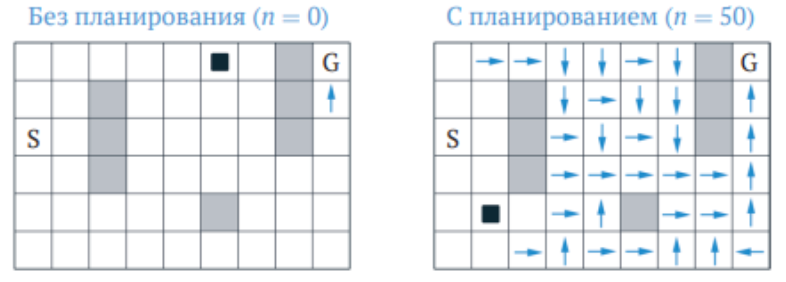
\includegraphics[width=0.9\textwidth]{8.1.png}
    \caption*{Рис. 8.3. Стратегии, найденные планирующими и непланирующими агентами Dyna-Q
    к середине второго эпизода. Стрелки показывают жадные действия в каждом
    состоянии; если для некоторого состояния не показана ни одна стрелка, то
    ценности всех действий в нём одинаковы. Чёрным квадратиком обозначено
    местоположение агента.}
\end{figure}

\begin{solution}
    Нет. Ни один многошаговый метод из главы 7 не сравняется с Dyna.

    Дело в том, какие пары состояние-действие обновляет каждый метод.
    Многошаговый метод обновляет только пары на реально пройденной траектории:
    чтобы изменить ценность состояния, в него надо физически прийти ногами.
    Dyna же на каждом реальном шаге делает $n$ планирующих обновлений (здесь
    $n=50$), выбирая из модели любые ранее встреченные пары --- то есть
    обновляет и те состояния, где агента сейчас нет, не заходя в них заново.
    Поэтому на рис. 8.3 у Dyna к середине второго эпизода уже выстроена цепочка
    жадных действий через половину лабиринта, а у одношагового агента изменился
    лишь последний шаг.

    Можно возразить, что самый сильный многошаговый метод --- Монте-Карло
    ($n\to\infty$) --- в конце эпизода обновит сразу всю траекторию. Но и это
    не помогает. Во-первых, МК заперт на одной буквально пройденной траектории
    и не умеет склеивать переходы в маршруты, которые целиком не проходились.
    Во-вторых, первый эпизод длинный и сильно петляет (около $1700$ шагов), а
    при $\gamma=0.95$ отдача состояния, посещённого в начале такого пути, равна
    $\gamma^{\approx 1700}\approx 0$: сигнал от цели до него практически не
    доходит, и выученная ценность отражает не кратчайший путь, а долгие
    блуждания. Планирующие обновления Dyna вида
    $Q(s,a)\leftarrow R+\gamma\max_a Q(s',a')$ за счёт оператора $\max$
    распространяют ценность назад по кратчайшему маршруту через модель.

    Итог: многошаговый бутстрэппинг обгонит одношаговый метод, но догнать Dyna
    не сможет.
\end{solution}

\subsection{Упражнение 8.2(с. 206)}
По какой причине Dyna-агент с призом за исследование, Dyna-Q+, показывает
лучшие результаты и в первой, и во второй частях экспериментов с блокированием и коротким путём?

\begin{solution}
    Dyna-Q+ хранит для каждой пары состояние-действие счётчик $\tau$ --- число
    шагов с момента, когда её последний раз пробовали в реальной среде, --- и на
    шаге планирования прибавляет к смоделированному вознаграждению бонус
    $\kappa\sqrt{\tau}$. Принцип один на обе части: где агент давно не был,
    $\tau$ велик, бонус большой, и жадная политика сама тянет проверить это
    место. Получается направленное исследование вместо случайного.

    Первая часть, до изменения среды. В начале обучения агент потрогал лишь
    малую долю пар, а у остальных $\tau$ только растёт, поэтому бонус заставляет
    систематически пробовать непройденные действия. Так Dyna-Q+ быстро строит
    полную модель и раньше выходит на оптимальный путь. Обычный Dyna-Q
    исследует только вслепую, случайными $\varepsilon$-жадными шагами, и
    покрывает пространство медленнее --- отсюда его более низкая кривая ещё до
    всякого изменения.

    Вторая часть, после изменения. В заброшенном участке $\tau$ растёт, бонус
    надувает ценность давно не пробованного действия, ведущего туда; агент идёт
    его проверить и из реального опыта узнаёт о перемене. Здесь важна асимметрия
    двух задач. При блокировании старый путь перестаёт работать, и среда сама
    вынуждает даже обычный Dyna-Q переучиться. А при коротком пути старый
    маршрут по-прежнему ведёт к цели, давления нет: модель Dyna-Q утверждает,
    что прохода не существует, и чем дольше он планирует, тем сильнее жадная
    политика отворачивается от нужного угла. Случайно набрать целую
    последовательность шагов в ту сторону почти невозможно, поэтому короткий
    путь обычный Dyna-Q не находит никогда. Бонус Dyna-Q+ именно это и
    исправляет: он нужен, чтобы замечать не только ухудшения среды, но и её
    улучшения, которые иначе остаются незамеченными. Любопытство стоит лишних
    проверочных шагов, но в этих задачах окупается.
\end{solution}

\subsection{Упражнение 8.3(с. 206)}
Если внимательно посмотреть на рис. 8.5, то можно заметить, что различие между
агентами Dyna-Q+ и Dyna-Q немного меньше в первой части эксперимента. Чем это
можно объяснить?

\begin{figure}[H]
    \centering
    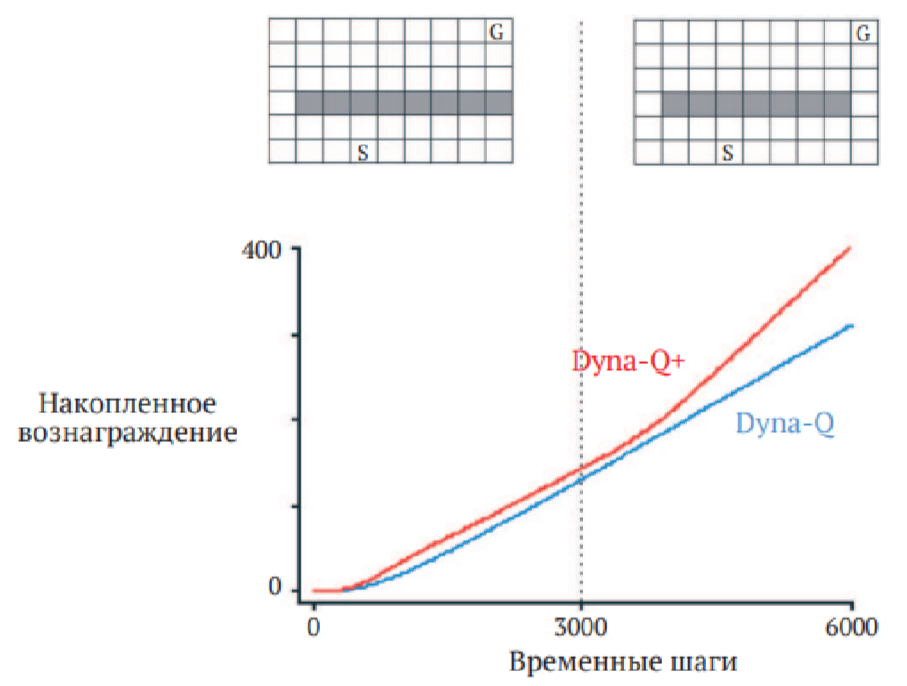
\includegraphics[width=0.75\textwidth]{fig_8_5.png}
    \caption*{Рис. 8.5. Усреднённые результаты Dyna-агентов в задаче о коротком пути в
    лабиринте. На протяжении первых 3000 шагов использовалась левая окружающая
    среда, а затем правая.}
\end{figure}

\begin{solution}
    Меньший зазор в первой части объясняется тем, что там исследованию почти
    нечего находить: среда статична, а полезный путь всего один. Преимущество
    Dyna-Q+ здесь узкое --- оно целиком за счёт более быстрого первичного
    обучения. Пока маршрут ещё не известен, бонус $\kappa\sqrt{\tau}$ заставляет
    агента систематически перебирать непройденные пары, и он покрывает лабиринт
    быстрее, чем обычный Dyna-Q со своими случайными $\varepsilon$-жадными
    шагами. Поэтому Dyna-Q+ находит оптимальный путь раньше и раньше начинает
    набирать вознаграждение оптимальным темпом --- эта фора и сдвигает его
    кривую вверх.

    Но как только путь найден, исследование перестаёт окупаться и даже начинает
    стоить: счётчик $\tau$ у давно не тронутых пар растёт, и бонус рано или
    поздно перерастает ценность оптимального действия, уводя агента на
    бессмысленный крюк. Поэтому фора сохраняется, но не увеличивается, и в
    статичной первой части агенты идут почти вровень. Разница резко растёт лишь
    во второй части, когда открывается короткий путь: тогда то же направленное
    исследование находит новый маршрут, которого обычный Dyna-Q не обнаруживает
    вовсе.
\end{solution}

\subsection{Упражнение 8.4(с. 206)}
Описанный выше приз за исследование
фактически изменяет оценки ценностей состояний и действий. Так ли это
необходимо? Предположим, что приз $\kappa\sqrt{\tau}$ используется не при
обновлении, а только при выборе действий, т.\,е. что всегда выбирается такое
действие, для которого $Q(S_t,a)+\kappa\sqrt{\tau(S_t,a)}$ достигает максимума.
Проведите эксперимент в сеточном мире, который демонстрирует сильные и слабые
стороны такого подхода.

\begin{solution}
    \textbf{Код смотри в отдельном файле репозитория.}

    Эксперимент поставлен на лабиринте с коротким путём (как в примере 8.3):
    сетка $6\times 9$, на шаге $5000$ из $10000$ справа от барьера открывается
    короткий путь, длинный при этом остаётся. Сравниваются три агента --- Dyna-Q,
    Dyna-Q+ и предложенный вариант, где приз входит только в правило выбора
    $\arg\max_a\!\big[Q(s,a)+\kappa\sqrt{\tau(s,a)}\big]$, но не в обновления.
    Параметры стандартные ($n=50$, $\alpha=1$, $\gamma=0.95$, $\varepsilon=0.1$,
    $\kappa=10^{-3}$), усреднение по $30$ запускам.

    \begin{figure}[ht]
        \centering
        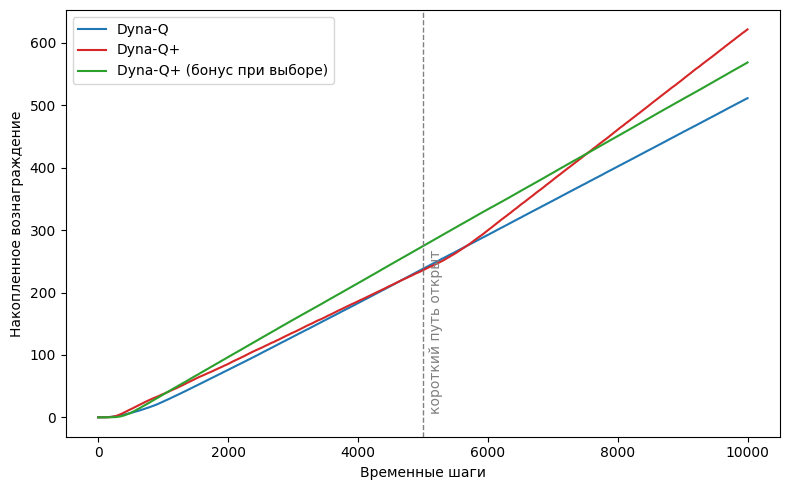
\includegraphics[width=0.75\textwidth]{8_4_sol_1.png}
        \caption*{Накопленное вознаграждение. Короткий путь открывается на шаге
        $5000$ (пунктир).}
    \end{figure}

    \begin{figure}[ht]
        \centering
        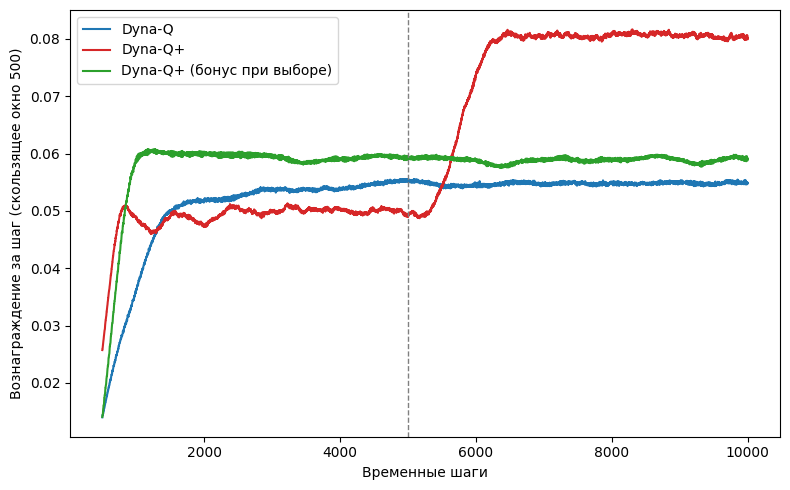
\includegraphics[width=0.75\textwidth]{8_4_sol_2.png}
        \caption*{Вознаграждение за шаг (скользящее окно $500$), тот же
        эксперимент.}
    \end{figure}

    Удобнее читать график вознаграждения за шаг (второй рисунок) --- на нём видны
    оба режима.

    Сильная сторона (статичная первая фаза, до шага $5000$). Здесь исследовать
    почти нечего, и селективный вариант (зелёный) даёт самый высокий темп
    вознаграждения, а полный Dyna-Q+ (красный) --- самый низкий. Причина в том,
    что у селективного варианта $Q$ остаётся честной оценкой ценности: приз не
    вшит в неё, поэтому, найдя путь, агент чисто его эксплуатирует. У Dyna-Q+
    приз распространяется через планирование и раздувает ценности давно не
    тронутых пар, из-за чего даже жадное действие периодически оказывается
    крюком, и агент чаще сходит с оптимального маршрута. Значит, в статичной
    среде менять оценки ценностей не только не нужно, но и слегка вредно.
    (Селективный вариант обгоняет и обычный Dyna-Q: его направленное локальное
    исследование быстрее выводит на путь и не платит постоянный
    $\varepsilon$-налог чисто случайных шагов.)

    Слабая сторона (после открытия прохода на шаге $5000$). Короткий путь лежит
    далеко от используемого маршрута, и находит его только Dyna-Q+: темп
    вознаграждения подскакивает с $\approx 0.05$ до $\approx 0.08$. Селективный
    вариант остаётся на уровне длинного пути ($\approx 0.06$), как и обычный
    Dyna-Q. Это прямо вытекает из устройства приза: в селективном варианте
    $\kappa\sqrt{\tau}$ влияет только на выбор в том состоянии, где агент стоит
    сейчас, и никуда не распространяется. Поэтому он не может выстроить градиент
    ценности, который провёл бы агента через весь лабиринт к заброшенному
    участку; а так как маршрут мимо этого участка не проходит, локальный стимул
    там попросту не срабатывает, и изменение остаётся незамеченным. У Dyna-Q+
    приз, вшитый в обновления, наоборот подтягивается к состояниям-предшественникам
    и целенаправленно ведёт агента к проходу.

    Вывод. Перенос приза в правило выбора --- это размен: мы получаем честные
    оценки ценности и чистую эксплуатацию (выигрыш в статичной среде и там, где
    переучиться вынуждает сама среда), но теряем способность дотягиваться до
    далёких неисследованных областей (проигрыш, когда находку надо искать там,
    куда текущая стратегия не ходит). Так что изменять оценки ради хорошего
    поведения в общем случае не обязательно --- но именно это изменение и
    обеспечивает дальнобойное направленное исследование, без которого далёкие
    улучшения среды не обнаруживаются.
\end{solution}

\subsection{Упражнение 8.5(с. 206)}
Как можно было бы изменить табличный алгоритм Dyna-Q на стр.~201, чтобы он был
применим к стохастической окружающей среде? Почему такая модификация могла бы
показывать плохие результаты в изменяющейся окружающей среде типа рассмотренной
в этом разделе? Как можно было бы изменить алгоритм, чтобы он хорошо работал и в
стохастической, и в изменяющейся среде?

\begin{solution}
    Часть 1 (стохастическая среда). Вместо детерминированной модели
    $Model(S,A)\leftarrow R,S'$ хранить для каждой пары $(s,a)$ выборочную оценку
    распределения исходов $\hat p(s',r\mid s,a)$ --- например, счётчики
    наблюдённых пар $(s',r)$. На шаге планирования вместо единственного
    сохранённого перехода сэмплировать $(s',r)$ из этой оценки (либо делать
    ожидаемое обновление по всем исходам).

    Часть 2 (почему плохо в изменяющейся среде). Выборочная оценка усредняет всю
    историю с равными весами. После изменения среды накопленные старые
    наблюдения подавляют немногие новые, и оценка сдвигается к новой динамике
    крайне медленно. Это даже хуже детерминированного Dyna-Q: там шаг
    $Model(S,A)\leftarrow R,S'$ --- перезапись, и одно новое наблюдение мгновенно
    исправляет модель, тогда как усреднение ещё долго тянет устаревшую статистику
    и заставляет агента планировать по ней.

    Часть 3 (и стохастическая, и изменяющаяся). Нужны два независимых
    исправления, закрывающие разные беды.

    \emph{Забывание.} Оценку распределения обновлять с постоянным шагом $\beta$,
    сдвигая весь вектор вероятностей к индикатору $e_{(S',R)}$ наблюдённого
    исхода:
    \begin{equation*}
        \hat p(\cdot\mid S,A)\leftarrow (1-\beta)\,\hat p(\cdot\mid S,A)
        + \beta\, e_{(S',R)}.
    \end{equation*}
    Это выпуклая комбинация двух распределений, поэтому результат снова
    неотрицателен и суммируется в единицу (перенормировка не нужна), а старые
    наблюдения гаснут геометрически --- модель отслеживает свежую динамику (как
    постоянный шаг для нестационарной задачи из главы~2).

    \emph{Исследование.} Добавить приз Dyna-Q+: на шаге планирования прибавлять к
    награде $\kappa\sqrt{\tau(s,a)}$, где $\tau$ --- число шагов с последнего
    реального опробования $(s,a)$.

    Забывание чинит переходы, которые агент \emph{уже наблюдает заново}; приз
    гонит его вернуться к тем, которые он \emph{перестал посещать}. Поодиночке ни
    одно не справляется, вместе --- метод тянет обе сложности сразу.

    \begin{algorithm}[H]
        \DontPrintSemicolon
        \SetKwInOut{Init}{Инициализация}
        \Init{$Q(s,a)$, оценки $\hat p(\cdot\mid s,a)$, счётчики
              $\mathrm{last}(s,a)\leftarrow 0$, время $t\leftarrow 0$}
        \While{\textnormal{обучение продолжается}}{
            $S\leftarrow$ текущее состояние\;
            $A\leftarrow \varepsilon\text{-жадная}(S,Q)$\;
            Выполнить $A$; наблюдать $R,S'$\;
            $Q(S,A)\leftarrow Q(S,A)+\alpha\big[R+\gamma\max_a Q(S',a)-Q(S,A)\big]$\;
            $\hat p(\cdot\mid S,A)\leftarrow (1-\beta)\,\hat p(\cdot\mid S,A)+\beta\,e_{(S',R)}$ \tcp*{забывающая модель}
            $t\leftarrow t+1$;\quad $\mathrm{last}(S,A)\leftarrow t$\;
            \For{$n$ \textnormal{раз}}{
                $\bar S\leftarrow$ случайное ранее наблюдавшееся состояние\;
                $\bar A\leftarrow$ случайное ранее предпринятое в $\bar S$ действие\;
                $(\bar S',\bar R)\sim \hat p(\cdot\mid \bar S,\bar A)$ \tcp*{сэмпл из распределения}
                $\bar R\leftarrow \bar R+\kappa\sqrt{t-\mathrm{last}(\bar S,\bar A)}$ \tcp*{приз за исследование}
                $Q(\bar S,\bar A)\leftarrow Q(\bar S,\bar A)+\alpha\big[\bar R+\gamma\max_a Q(\bar S',a)-Q(\bar S,\bar A)\big]$\;
            }
        }
    \end{algorithm}
\end{solution}

\subsection{Упражнение 8.6(с. 213)}
В приведённом выше анализе предполагалось, что все $b$ возможных следующих
состояний равновероятны. Предположим вместо этого, что распределение сильно
несимметрично, т.\,е. некоторые из $b$ состояний возникают с гораздо большей
вероятностью, чем другие. При таком предположении увеличится или уменьшится
преимущество выборочных обновлений над полными? Аргументируйте свой ответ.

\begin{solution}
    Преимущество выборочных обновлений увеличится.

    Полное обновление суммирует по всем $b$ преемникам и стоит порядка $b$
    операций независимо от их вероятностей: на маловероятные исходы оно тратится
    наравне с частыми, хотя вклад первых в ожидание ничтожен. Скос распределения
    эту цену не снижает.

    Выборочное обновление сэмплирует $s'\sim p(\cdot\mid s,a)$, то есть само
    вкладывает вычисления пропорционально вероятности исхода (а значит, и его
    вкладу в ожидание). При сильном скосе масса собрана на немногих состояниях:
    почти все сэмплы попадают в них, разброс сэмплированной цели мал, и среднее
    приближается к истинному ожиданию
    $\sum_{s'} p(s'\mid s,a)\,[\,r+\gamma\max_a Q(s',a)\,]$ за число обновлений,
    много меньшее $b$. Маловероятные исходы при этом недооцениваются --- но они и
    должны влиять слабо, ведь их вес $p$ мал.

    Итого: при скосе выборочное обновление достигает хорошей оценки ещё быстрее,
    тогда как полное по-прежнему платит полную цену $b$. Разрыв в пользу
    выборочного растёт.
\end{solution}

\subsection{Упражнение 8.7(с. 216)}
Некоторые графики на рис.~8.8 имеют всплески и неровности на ранних участках,
особенно это относится к верхнему графику для случая $b=1$ и равномерного
распределения. Как это можно объяснить? Какие аспекты представленных данных
подтверждают вашу гипотезу?

\begin{figure}[H]
    \centering
    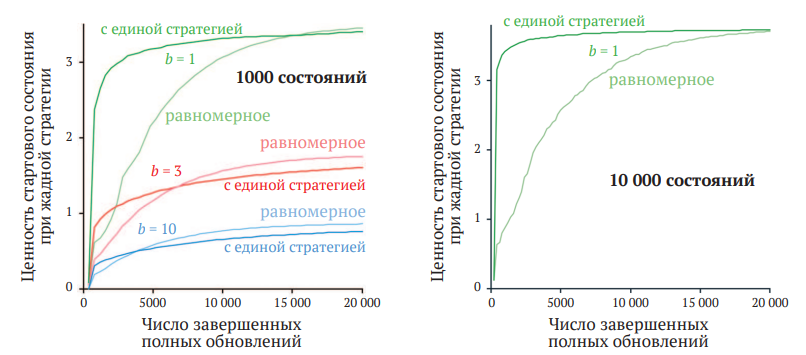
\includegraphics[width=0.95\textwidth]{fig_8_8.png}
    \caption*{Рис. 8.8. Относительная эффективность обновлений, распределённых равномерно в
    пространстве состояний, и обновлений, в которых используются имитированные
    траектории с единой стратегией. Все эпизоды начинаются в одном и том же
    состоянии. Результаты соответствуют случайно сгенерированным задачам двух
    разных размеров с различными коэффициентами ветвления $b$.}
\end{figure}

\begin{solution}
    По оси ординат отложена ценность стартового состояния при жадной стратегии,
    пересчитываемая по мере накопления полных обновлений. Эта ценность зависит
    только от состояний на жадном пути из старта. При равномерном распределении
    обновляются все пары подряд, но на ценность старта влияют лишь немногие из
    них, и срабатывают они в произвольном порядке, пока
    значения ещё не устоялись: кривая стоит ровно, а затем подскакивает, когда
    очередное релевантное звено обновилось или сменилось жадное действие. При
    $b=1$ каждое полное обновление одношаговое (цель $r+\gamma\max_a Q(s')$ по
    единственному преемнику, без усреднения), поэтому такие скачки особенно
    резкие.

    Гипотезу подтверждают два наблюдения. Во-первых, всплески монотонно слабеют с
    ростом $b$: при $b=1$ они выражены, при $b=3$ тише, при $b=10$ кривая почти
    гладкая --- это согласуется с тем, что при большем ветвлении цель усредняется
    по $b$ преемникам (каждый с весом $\sim 1/b$), и изменение одного из них
    двигает её лишь на малую долю. Во-вторых, неровности сидят только на раннем
    участке, а дальше все кривые выходят на плато: эффект переходный и гаснет по
    мере того, как ценности сходятся к истинным и обновления перестают что-либо
    менять.
\end{solution}

\subsection{Упражнение 8.8(с. 224)}
Повторите эксперимент, результаты которого
представлены в нижней части рис.~8.8, а затем попробуйте выполнить его же со
значением $b=3$. Обсудите полученные результаты.

\begin{solution}
    \textbf{Код смотри в отдельном файле репозитория.}

    Воспроизведён эксперимент для задачи с 10000 состояний: случайная MDP с
    ветвлением $b$, обрывом эпизода с вероятностью 0.1 и наградами из $N(0,1)$,
    полные обновления (8.1) с $\gamma=0.9$. Сравниваются равномерное распределение
    обновлений (перебор всех пар в перемешанном порядке) и распределение с единой
    $\varepsilon$-жадной стратегией из старта; по оси ординат --- ценность старта
    при жадной стратегии (оценка Монте-Карло), усреднение по 20 задачам. Случай
    $b=1$ повторяет нижнюю панель рис.~8.8, случай $b=3$ достроен.

    \begin{figure}[h]
        \centering
        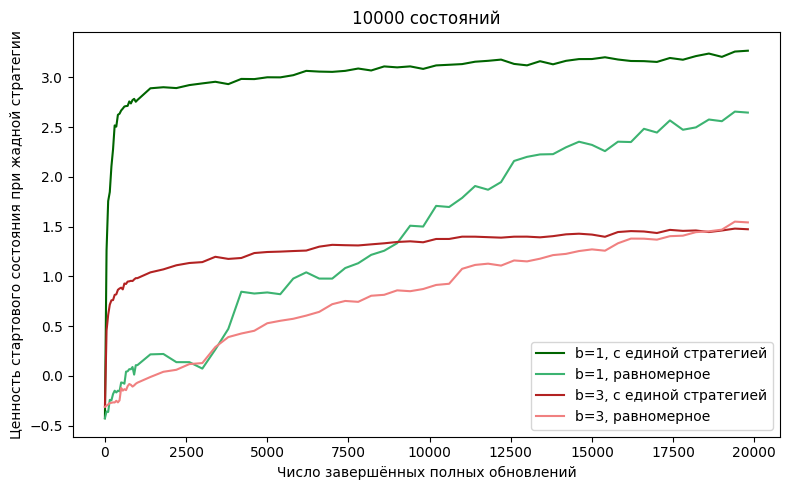
\includegraphics[width=0.8\textwidth]{fig_8_8_sol.png}
        \caption*{Задача с 10000 состояний: равномерное распределение обновлений
        против распределения с единой стратегией, для $b=1$ и $b=3$.}
    \end{figure}

    При $b=1$ распределение с единой стратегией даёт большое и продолжительное
    преимущество: оно сразу концентрирует обновления на немногих состояниях,
    достижимых из старта, поэтому ценность старта взлетает за первые сотни
    обновлений. Равномерному же на 10000 состояний 20000 обновлений хватает лишь
    на один полный проход по всем парам, поэтому значения распространяются
    медленно, и кривая догоняет единую стратегию только к концу.

    При $b=3$ это преимущество резко сжимается: кривая с единой стратегией рано
    выходит на низкое плато, а равномерное к концу её догоняет и даже слегка
    обгоняет. Причина --- рост ветвления: при $b=3$ траектории из старта быстро
    разветвляются и охватывают гораздо более широкое множество состояний, так что
    фокусировка единой стратегии на окрестности старта размывается; вдобавок
    достижимая ценность ниже (плато $b=3$ заметно ниже, чем у $b=1$).

    Вывод согласуется с общим утверждением раздела: выигрыш распределения с единой
    стратегией максимален, когда состояний много, а ветвление мало, и с ростом
    $b$ он быстро тает.
\end{solution}


\newpage
\part{Приближенные методы решения}

\part{Приближенные методы решения}
\section{Глава 9. Предсказание с единой стратегией и аппроксимацией}

\subsection{Упражнение 9.1(с. 252)}
Покажите, что табличные методы типа тех, что представлены в первой части книги, --- частный случай линейной аппроксимации функции. Каковы в этом случае векторы признаков?
\begin{solution}
    Возьмём $d=|\mathcal S|$ и в качестве признаков --- one-hot векторы: для
    состояния $s$
    \begin{equation*}
        x_i(s) = \begin{cases} 1, & i = s,\\ 0, & i \ne s, \end{cases}
        \qquad i = 1, \dots, |\mathcal S|.
    \end{equation*}
    Каждому состоянию отвечает свой базисный вектор, и все они ортонормированы.

    При таких признаках линейная аппроксимация (9.8) вынимает ровно одну
    компоненту весов:
    \begin{equation*}
        \hat v(s, \mathbf w) = \mathbf w^\top \mathbf x(s)
        = \sum_{i=1}^{|\mathcal S|} w_i x_i(s) = w_s.
    \end{equation*}
    То есть вектор весов $\mathbf w$ --- это и есть таблица ценностей, а $w_s$ ---
    ячейка состояния $s$.

    Метод тоже вырождается в табличный. Градиент здесь $\nabla\hat v(s,\mathbf w)
    = \mathbf x(s)$, поэтому общее линейное СГС-обновление
    \begin{equation*}
        \mathbf w_{t+1} = \mathbf w_t + \alpha\big[U_t - \hat v(S_t,\mathbf w_t)\big]\mathbf x(S_t)
    \end{equation*}
    из-за one-hot $\mathbf x(S_t)$ затрагивает единственную компоненту $i=S_t$, а
    все остальные ($i\ne S_t$) оставляет без изменения:
    \begin{equation*}
        w_{S_t} \leftarrow w_{S_t} + \alpha\big[U_t - w_{S_t}\big],
        \qquad w_i \leftarrow w_i \ (i \ne S_t).
    \end{equation*}
    Это дословно табличное обновление с целью $U_t$ (например, $U_t = G_t$ для
    Монте-Карло или $U_t = R_{t+1} + \gamma\hat v(S_{t+1},\mathbf w_t)$ для TD(0)).
    Обновления разных состояний не влияют друг на друга --- ровно потому, что
    признаки ортогональны, --- так что обобщения между состояниями нет, как и
    положено таблице.
\end{solution}

\subsection{Упражнение 9.2(с. 253)}
Почему формула (9.17) определяет $(n+1)^k$ различных признаков для размерности
$k$?
\begin{equation}
    x_i(s) = \prod_{j=1}^{k} s_j^{\,c_{i,j}},
    \tag{9.17}
\end{equation}
\begin{solution}
    Признак задаётся набором показателей $(c_1, \dots, c_k)$, где каждый
    $c_j$ независимо пробегает множество $\{0, 1, \dots, n\}$ из $n+1$ элементов.
    По правилу произведения таких наборов
    \begin{equation*}
        \underbrace{(n+1)(n+1)\cdots(n+1)}_{k} = (n+1)^k.
    \end{equation*}

    Осталось проверить, что разным наборам отвечают разные признаки (иначе
    различных признаков было бы меньше). Пусть два набора задают один и тот же
    моном при всех значениях аргументов:
    \begin{equation*}
        \prod_{j=1}^{k} s_j^{c_j} = \prod_{j=1}^{k} s_j^{c'_j}
        \quad \text{для всех } s_1, \dots, s_k.
    \end{equation*}
    Зафиксируем все аргументы кроме $s_j$, положив их равными $1$. Слева и справа
    остаётся $s_j^{c_j} = s_j^{c'_j}$ при всех $s_j$, откуда $c_j = c'_j$. Это
    верно для каждого $j$, поэтому наборы совпадают.

    Значит, отображение из наборов показателей в признаки инъективно: различных
    наборов $(n+1)^k$, и различных признаков ровно столько же.
\end{solution}

\subsection{Упражнение 9.3 (с. 254)}
При каких $n$ и $c_{i,j}$ порождаются векторы признаков
\begin{equation*}
    \mathbf x(s) = \big(1,\ s_1,\ s_2,\ s_1 s_2,\ s_1^2,\ s_2^2,\ s_1 s_2^2,\ s_1^2 s_2,\ s_1^2 s_2^2\big)^\top ?
\end{equation*}

\begin{solution}
    Здесь $k=2$ (две компоненты $s_1, s_2$), и каждый признак имеет вид
    $x_i(s) = s_1^{c_{i,1}} s_2^{c_{i,2}}$. Признаков ровно $9 = 3^2 = (n+1)^k$,
    причём это все комбинации показателей из $\{0,1,2\}^2$ --- то есть полный
    полиномиальный базис порядка $n=2$ (показатели $c_{i,j} \in \{0,1,2\}$).

    По порядку признаков пары показателей $(c_{i,1}, c_{i,2})$ таковы:
    \begin{equation*}
        \begin{array}{c|ccccccccc}
            x_i(s) & 1 & s_1 & s_2 & s_1 s_2 & s_1^2 & s_2^2 & s_1 s_2^2 & s_1^2 s_2 & s_1^2 s_2^2 \\
            \hline
            (c_{i,1}, c_{i,2}) & (0,0) & (1,0) & (0,1) & (1,1) & (2,0) & (0,2) & (1,2) & (2,1) & (2,2)
        \end{array}
    \end{equation*}
\end{solution}

\subsection{Упражнение 9.4(с. 264)}
Допустим, у нас есть основания полагать, что одно из двух измерений пространства состояний оказывает большее влияние на функцию ценности, чем другое, и что обобщение должно производиться главным образом поперёк этого измерения, а не вдоль него. Какого рода замощения можно было бы предложить, чтобы извлечь пользу из этого априорного знания?

\begin{solution}
    Пусть важная ось (вдоль которой функция ценности меняется быстро) --- это
    $y$, а маловажная --- $x$. Предлагаются плитки в виде узких горизонтальных
    полос: вытянутых вдоль $x$ и узких по $y$.

    Такая форма сразу даёт нужную асимметрию обобщения. При смещении вдоль $x$
    (вдоль полосы) состояние почти всегда остаётся в той же плитке, набор
    активных признаков не меняется, поэтому оценка вдоль $x$ почти постоянна ---
    широкое обобщение по маловажной оси. При смещении по $y$ (поперёк полос)
    из-за их узости состояние быстро переходит из одной полосы в другую, активные
    плитки меняются, и оценка может меняться резко --- слабое обобщение, высокое
    разрешение по важной оси.

    Форма плитки задаёт обобщение, но итоговое разрешение определяется тем,
    насколько густо наслаиваются смещённые замощения. Поэтому замощения нужно
    сдвигать в основном вдоль $y$: чем гуще сдвиг по $y$, тем больше различимых
    комбинаций активных плиток вдоль этой оси и тем тоньше разрешение там, где оно
    важно. Вдоль $x$ сдвиги не нужны или редки --- там разрешение намеренно грубое,
    и лишние замощения только тратили бы память.

    Итого: узкие горизонтальные полосы, смещаемые преимущественно вдоль $y$ и
    почти не смещаемые вдоль $x$. Это даёт широкое обобщение по маловажной оси $x$
    и тонкое разрешение по важной оси $y$ --- ровно то, что подсказывает априорное
    знание.
\end{solution}

\subsection{Упражнение 9.5(с. 266)}
Предположим, что плиточное кодирование используется для преобразования
семимерного непрерывного пространства состояний в бинарные векторы признаков с
целью оценивания функции ценности состояния $\hat v(s,\mathbf w)\approx
v_\pi(s)$. Есть основания полагать, что зависимость между измерениями слабая,
поэтому мы решаем использовать восемь замощений по каждому измерению в
отдельности (полосами), т.\,е. всего $7\times 8 = 56$ замощений. Кроме того, на
случай, если между измерениями имеются какие-то попарные зависимости, мы берём
все $21$ пару измерений и для каждой пары строим по два замощения прямоугольными
плитками. Всего получается $21\times 2 + 56 = 98$ замощений. Имея эти векторы
признаков, мы всё же подозреваем, что следует применить усреднение для устранения
шума, поэтому решаем, что обучение должно быть постепенным, т.\,е. один и тот же
вектор признаков должен предъявляться примерно $10$ раз, прежде чем обучение
выйдет на асимптоту. Как следует выбрать размер шага $\alpha$? Объясните свой
ответ.

\begin{solution}
    Используем эвристику (9.19): $\alpha = \big(\tau\,\mathbb E[\mathbf x^\top
    \mathbf x]\big)^{-1}$. Здесь важно не число замощений само по себе, а
    $\mathbf x^\top\mathbf x$ --- число активных признаков (единиц в векторе).

    В каждом замощении, независимо от формы плиток (полоса или прямоугольник),
    состояние попадает ровно в одну плитку и активирует ровно один признак.
    Поэтому число активных признаков равно числу замощений:
    \begin{equation*}
        \mathbf x^\top\mathbf x = 56 + 21\cdot 2 = 98.
    \end{equation*}
    То, что прямоугольные замощения «двумерные», на это число не влияет.

    Причём $\mathbf x^\top\mathbf x$ здесь не случайно, а тождественно равно $98$ в
    любом состоянии (по одной активной плитке на замощение всегда). Это ровно тот
    идеальный случай из текста, когда $\mathbf x^\top\mathbf x$ постоянно, так что
    $\mathbb E[\mathbf x^\top\mathbf x] = 98$ и эвристика точна, а не приближённа.

    Подставляя $\tau = 10$:
    \begin{equation*}
        \alpha = \frac{1}{\tau\,\mathbf x^\top\mathbf x} = \frac{1}{10\cdot 98}
        = \frac{1}{980}.
    \end{equation*}
\end{solution}

\section{Глава 10. Управление с единой стратегией и аппроксимацией}

\subsection{Упражнение 10.1(с. 294)}
В этой главе мы не рассматривали явно и не приводили псевдокод для методов
Монте-Карло. На что они были бы похожи? Почему не имеет смысла приводить для них псевдокод? Какие результаты они дали бы в задаче о машине на горе?

\begin{solution}
    На что похожи. Метод Монте-Карло --- это частный случай уже приведённого
    $n$-шагового полуградиентного Sarsa, когда окно дотягивается до конца
    эпизода. При $t+n\ge T$ бутстрэп-член в (10.4) исчезает и цель становится
    полным доходом: $G_{t:t+n}=G_t$. Обновление превращается в
    \begin{equation*}
        \mathbf w \leftarrow \mathbf w + \alpha\big[G_t - \hat q(S_t, A_t, \mathbf w)\big]\nabla\hat q(S_t, A_t, \mathbf w),
    \end{equation*}
    применяемое ко всем парам эпизода после его завершения.

    Почему не нужен отдельный псевдокод. Именно потому, что MC не требует ничего
    нового: он буквально получается из $n$-шагового Sarsa, если взять $n$
    настолько большим, что цель всегда становится полным доходом $G_t$. Отдельная
    запись лишь повторила бы уже имеющуюся.

    Результаты на машине на горе. Здесь MC проявил бы себя плохо, и причина
    глубже, чем медленная сходимость. MC обновляет ценности только по завершении
    эпизода --- до этого $G_t$ не определён. Значит весь первый эпизод агент
    блуждает с замороженной начальной политикой и не делает ни одного обновления.
    А при оптимистичном старте ($\mathbf w=0$) и слабой стартовой политике нет
    гарантии, что эпизод завершится в разумное время; в худшем случае MC не
    сделает ни одного обновления вовсе.

    Sarsa этой ловушки лишён: он обновляет $\hat q$ прямо во время эпизода, и эти
    обновления помогают довести эпизод до конца. Поэтому на рис.~10.3 даже первый
    эпизод Sarsa (длиной более 1000 шагов) завершается --- но именно потому, что
    политика улучшается по ходу; переносить эту завершаемость на MC с его
    замороженной политикой нельзя.

    Наконец, даже когда эпизоды завершаются, MC обновляется лишь раз за эпизод по
    полному доходу через тысячи шагов: сигнал размыт, оценки шумные, обучение
    крайне медленное. Бутстрэппинг $n$-шагового Sarsa даёт информативные
    обновления на каждом шаге --- поэтому лучший результат приходится на
    промежуточные $n$ (рис.~10.4), а MC ($n\to\infty$) оказывается наихудшим
    краем. Ключевое преимущество, которого MC лишён, --- возможность учиться внутри ещё не завершённого эпизода.
\end{solution}

\subsection{Упражнение 10.2(с. 294)}
Напишите псевдокод полуградиентного одношагового метода Expected Sarsa для
задачи управления.

\begin{solution}
    Отличие от одношагового Sarsa в цели обновления: вместо $\gamma\,\hat
    q(S',A')$ берётся матожидание по политике $\gamma\sum_a \pi(a\mid S')\hat
    q(S',a,\mathbf w)$. Поскольку конкретное $A'$ в цель больше не входит,
    заранее выбирать и хранить следующее действие не нужно --- действие
    выбирается в начале каждого шага по текущему $\hat q$. В задаче управления
    $\pi$ --- та же $\varepsilon$-жадная по $\hat q(S',\cdot)$ политика, которой
    следует агент (вес $1-\varepsilon+\varepsilon/|\mathcal A|$ на жадном действии
    и $\varepsilon/|\mathcal A|$ на каждом из остальных).

    \begin{algorithm}[H]
        \DontPrintSemicolon
        \SetKwInOut{Input}{Вход}
        \SetKwInOut{Param}{Параметры}
        \Input{дифференцируемая параметризация $\hat q:\mathcal S\times\mathcal A\times\mathbb R^d\to\mathbb R$}
        \Param{размер шага $\alpha>0$, небольшое $\varepsilon>0$}
        Инициализировать веса $\mathbf w\in\mathbb R^d$ произвольно (например, $\mathbf w=\mathbf 0$)\;
        \For{\textnormal{каждого эпизода}}{
            $S\leftarrow$ начальное состояние эпизода\;
            \While{$S$ \textnormal{не заключительное}}{
                Выбрать $A$ как $\varepsilon$-жадное относительно $\hat q(S,\cdot,\mathbf w)$\;
                Предпринять действие $A$; наблюдать $R,S'$\;
                \eIf{$S'$ \textnormal{заключительное}}{
                    $\delta\leftarrow R-\hat q(S,A,\mathbf w)$\;
                }{
                    $\delta\leftarrow R+\gamma\sum_a \pi(a\mid S')\,\hat q(S',a,\mathbf w)-\hat q(S,A,\mathbf w)$\;
                }
                $\mathbf w\leftarrow \mathbf w+\alpha\,\delta\,\nabla\hat q(S,A,\mathbf w)$\;
                $S\leftarrow S'$\;
            }
        }
    \end{algorithm}

    Здесь $\pi(\cdot\mid S')$ --- $\varepsilon$-жадная политика по $\hat
    q(S',\cdot,\mathbf w)$. Если вместо неё взять жадную политику, сумма
    вырождается в $\max_a \hat q(S',a,\mathbf w)$ --- это уже off-policy
    Q-обучение, другой алгоритм.
\end{solution}

\subsection{Упражнение 10.3(с. 294)}
Почему стандартная ошибка для результатов, показанных на рис.~10.4, выше при больших $n$, чем при малых?
\begin{figure}[H]
    \centering
    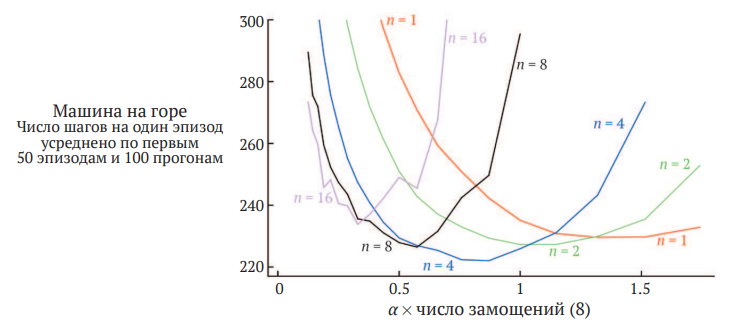
\includegraphics[width=1\linewidth]{fig_10_4.png}
    \caption{Рис. 10.4. Влияние $\alpha$ и $n$ на качество $n$-шагового полуградиентного Sarsa и аппроксимации функций посредством плиточного кодирования в задаче о машине на
    горе. Как обычно, наилучшее качество достигается при промежуточном уровне бутстрэппинга ($n=4$). Результаты приведены для избранных значений $\alpha$ в логарифмическом масштабе, а затем соединены прямыми линиями. Стандартная ошибка варьировалась от $0.5$ (меньше ширины линии) для $n=1$ до примерно $4$ для $n=16$, поэтому все основные эффекты статистически значимы.}
\end{figure}
\begin{solution}
    Стандартная ошибка здесь --- это $\sigma/\sqrt{N}$, разброс измеренной кривой
    между прогонами ($N=100$ для всех $n$, поэтому различие идёт от $\sigma$ ---
    дисперсии результата между отдельными прогонами).

    Источник --- дисперсия цели обновления. Цель $n$-шагового метода
    \begin{equation*}
        G_{t:t+n} = R_{t+1} + \gamma R_{t+2} + \dots + \gamma^{n-1} R_{t+n}
        + \gamma^n \hat q(S_{t+n}, A_{t+n}, \mathbf w)
    \end{equation*}
    при $n=16$ включает сумму шестнадцати реальных наград, набранных вдоль
    траектории, которая ветвится из-за случайного старта и $\varepsilon$-жадности.
    Чем длиннее этот случайный хвост до бутстрэп-члена, тем выше дисперсия самой
    цели: много случайных шагов накапливают разброс. При $n=1$ цель опирается на
    одну награду плюс бутстрэп и почти детерминирована. (Дисконтирование $\gamma^k$
    при этом гасит вклад далёких наград и работает на снижение дисперсии хвоста ---
    то есть ограничивает рост ошибки, а не вызывает его.)

    Высокодисперсная цель означает, что траектории весов в разных прогонах
    расходятся сильнее, поэтому «число шагов на эпизод» гуляет от прогона к прогону
    шире, и при том же $N$ стандартная ошибка $\sigma/\sqrt{N}$ выше.

    Усиливает эффект и то, что рис.~10.4 усредняет по первым 50 эпизодам --- по
    самой ранней, нестабильной фазе. Там политика и $\hat q$ ещё далеки от
    устойчивых, и длинные $n$-шаговые цели, вычисленные по ещё плохой $\hat q$,
    особенно сильно швыряют результат от прогона к прогону. Поэтому межпрогонная
    дисперсия (а с ней и стандартная ошибка) растёт с $n$ заметнее всего именно на
    этом раннем участке.
\end{solution}

\subsection{Упражнение 10.4(с. 296)}
Напишите псевдокод дифференциальной версии полуградиентного Q-обучения.

\begin{solution}
    Отличие от дифференциального полуградиентного Sarsa в цели: вместо
    $\hat q(S',A')$ берётся $\max_a \hat q(S',a)$ (off-policy, целевая политика ---
    жадная). Поэтому конкретное $A'$ заранее выбирать не нужно --- действие
    выбирается в начале каждого шага по текущему $\hat q$. Тот же $\delta$
    обновляет и веса, и оценку среднего вознаграждения $\bar R$.

    \begin{algorithm}[H]
        \DontPrintSemicolon
        \SetKwInOut{Input}{Вход}
        \SetKwInOut{Param}{Параметры}
        \Input{дифференцируемая параметризация $\hat q:\mathcal S\times\mathcal A\times\mathbb R^d\to\mathbb R$}
        \Param{размеры шагов $\alpha,\beta>0$}
        Инициализировать веса $\mathbf w\in\mathbb R^d$ произвольно (например, $\mathbf w=\mathbf 0$)\;
        Инициализировать оценку среднего вознаграждения $\bar R\in\mathbb R$ произвольно (например, $\bar R=0$)\;
        Инициализировать состояние $S$\;
        \For{\textnormal{каждого шага}}{
            Выбрать $A$ как $\varepsilon$-жадное относительно $\hat q(S,\cdot,\mathbf w)$\;
            Предпринять действие $A$; наблюдать $R,S'$\;
            $\delta\leftarrow R-\bar R+\max_a \hat q(S',a,\mathbf w)-\hat q(S,A,\mathbf w)$\;
            $\bar R\leftarrow \bar R+\beta\,\delta$\;
            $\mathbf w\leftarrow \mathbf w+\alpha\,\delta\,\nabla\hat q(S,A,\mathbf w)$\;
            $S\leftarrow S'$\;
        }
    \end{algorithm}

    Здесь $\bar R$ оценивает средний reward целевой (жадной) политики, поскольку
    $\delta$ построен вокруг $\max_a \hat q(S',a,\mathbf w)$. Это согласовано с
    обновлением весов, в которое входит та же $\bar R$.
\end{solution}

\subsection{Упражнение 10.5(с. 296)}
Какие уравнения (кроме 10.10) необходимы для определения дифференциальной версии алгоритма TD(0)?
\begin{equation}
    \delta_t \doteq R_{t+1} - \bar R_{t+1} + \hat v(S_{t+1}, \mathbf w_t) - \hat v(S_t, \mathbf w_t),
    \tag{10.10}
\end{equation}
\begin{solution}
    Дана дифференциальная TD-ошибка в $v$-форме (10.10):
    \begin{equation*}
        \delta_t = R_{t+1} - \bar R_{t+1} + \hat v(S_{t+1},\mathbf w_t) - \hat v(S_t,\mathbf w_t).
    \end{equation*}
    Кроме неё, для полного определения дифференциального TD(0) нужны ещё два
    уравнения обновления.

    Обновление весов (аналог (10.12), но с градиентом $\hat v$):
    \begin{equation*}
        \mathbf w_{t+1} = \mathbf w_t + \alpha\,\delta_t\,\nabla\hat v(S_t,\mathbf w_t).
    \end{equation*}

    Обновление оценки среднего вознаграждения:
    \begin{equation*}
        \bar R_{t+1} = \bar R_t + \beta\,\delta_t.
    \end{equation*}

    Дополнительно нужно оговорить две вещи. Во-первых, $\delta$ берётся именно в
    $v$-форме (10.10), а не в $q$-форме (10.11) --- то есть оценивается $v_\pi$.
    Во-вторых, это задача \emph{предсказания}: раз мы учим $\hat v$, а не $\hat q$,
    выбор действий по ней невозможен, поэтому политика $\pi$ фиксирована и задана
    извне, а действия просто берутся по ней (никаких правил выбора действия не
    требуется).

    Здесь обновление $\bar R$ через $\delta$ несмещённо, в отличие от
    дифференциального Q-обучения: TD(0) on-policy, $\delta$ построен вокруг $\hat
    v(S_{t+1})$ для той же политики $\pi$, по которой собираются данные, поэтому
    неподвижная точка $\mathbb E[\delta]=0$ даёт ровно $\bar R = r(\pi)$.
\end{solution}

\subsection{Упражнение 10.6(с. 297)}
Рассмотрим марковский процесс вознаграждения, состоящий из трёх состояний $A$, $B$, $C$; переходы производятся детерминированно по кругу. Вознаграждение $+1$ начисляется по прибытии в состояние $A$, в остальных случаях оно равно $0$. Каковы дифференциальные ценности всех трёх состояний?

\begin{solution}
    Цикл $A\to B\to C\to A$ детерминирован, поэтому $\mu(s)=\tfrac13$ для всех
    состояний, а среднее вознаграждение $r(\pi)=\tfrac13$ (одна награда $+1$ на
    три перехода).

    Дифференциальные ценности удовлетворяют уравнению Беллмана без обесценивания
    $v(s) = \big(r_{s\to s'}-r(\pi)\big)+v(s')$, где $+1$ начисляется на переходе,
    прибывающем в $A$ (то есть на $C\to A$):
    \begin{align*}
        v(A) &= \big(0-\tfrac13\big)+v(B),\\
        v(B) &= \big(0-\tfrac13\big)+v(C),\\
        v(C) &= \big(1-\tfrac13\big)+v(A).
    \end{align*}

    Каждое уравнение фиксирует лишь разность соседних ценностей, а их сумма даёт
    тождество $0=0$, поэтому независимых уравнений два на три неизвестных: система
    вырождена, и решение определено с точностью до общей аддитивной константы.
    Это и есть свойство дифференциальных ценностей --- значимы только их разности,
    а общий уровень произволен. Зафиксируем его нормировкой $\sum_s v(s)=0$ и
    получаем
    \begin{equation*}
        v(A) = -\tfrac13, \qquad v(B) = 0, \qquad v(C) = \tfrac13.
    \end{equation*}

    Смысл: ценность тем выше, чем скорее из состояния попадаешь в $A$ (где ждёт
    награда). Ближе всего к $A$ стоит $C$ (один шаг) --- у него ценность
    максимальна; дальше всего $A$ (целый цикл до следующей награды) --- минимальна.
    При другой нормировке (например, $v(A)=0$) получились бы те же разности,
    сдвинутые на константу: $v(A)=0,\ v(B)=\tfrac13,\ v(C)=\tfrac23$.
\end{solution}

\subsection{Упражнение 10.7(с. 298)}
Предположим, что имеется МППР, который при любой стратегии порождает
детерминированную бесконечную последовательность вознаграждений $+1, 0, +1, 0,
\dots$. Технически это недопустимо, потому что нарушается свойство эргодичности
--- не существует стационарного предельного распределения $\mu_\pi$ и предела
(10.7). Тем не менее среднее вознаграждение (10.6) определено корректно. Чему оно
равно? Теперь рассмотрим два состояния этого МППР. При старте из состояния $A$
последовательность вознаграждений точно такая, как описано выше, т.\,е. начинается
с $+1$, а при старте из $B$ последовательность вознаграждений начинается с $0$ и
продолжается так: $+1, 0, +1, 0, \dots$. В этом случае дифференциальный доход
(10.9) определён некорректно, потому что предела не существует. Чтобы исправить
ситуацию, можно было бы определить ценность состояния по-другому:
\begin{equation}
    v_\pi(s) \doteq \lim_{\gamma\to1}\lim_{h\to\infty}
    \sum_{t=0}^{h} \gamma^t\big(\mathbb E_\pi[R_{t+1}\mid S_0=s]-r(\pi)\big).
    \tag{10.13}
\end{equation}
Каковы ценности состояний $A$ и $B$ при таком определении?
\begin{solution}
    Среднее вознаграждение. По (10.6) это предел среднего по первым $h$ шагам.
    Сумма первых $h$ наград последовательности $+1,0,+1,0,\dots$ равна числу
    единиц среди них, то есть $h/2$ с точностью до $\pm\tfrac12$. Деля на $h$:
    \begin{equation*}
        r(\pi) = \lim_{h\to\infty}\frac1h\sum_{t=1}^h R_t
        = \lim_{h\to\infty}\Big(\tfrac12 \pm \tfrac{1}{2h}\Big) = \tfrac12.
    \end{equation*}
    Сдвиг фазы между стартами из $A$ и $B$ меняет частичную сумму лишь на единицу
    --- фиксированно, тогда как делим на растущее $h$, --- поэтому в пределе он
    вымывается, и $r(\pi)=\tfrac12$ для обоих стартов. При этом $r(\pi)$ существует,
    хотя $\mu_\pi$ и предел (10.7) --- нет: усреднение по времени работает там, где
    усреднение по стационарному распределению неприменимо.

    Ценности через (10.13). Из $A$ отклонения наград от $r(\pi)$ равны
    $\tfrac12(-1)^t$, $t=0,1,2,\dots$. Подставляя в (10.13) и пользуясь
    $\sum_{t=0}^\infty(-\gamma)^t = \tfrac{1}{1+\gamma}$ при $\gamma<1$:
    \begin{equation*}
        v(A) = \lim_{\gamma\to1}\sum_{t=0}^\infty \gamma^t\cdot\tfrac12(-1)^t
        = \lim_{\gamma\to1}\frac{1}{2(1+\gamma)} = \frac14.
    \end{equation*}
    Из $B$ отклонения равны $\tfrac12(-1)^{t+1}$, что даёт противоположный знак:
    \begin{equation*}
        v(B) = \lim_{\gamma\to1}\Big(-\frac{1}{2(1+\gamma)}\Big) = -\frac14.
    \end{equation*}

    Именно ради этого в (10.13) предел по $h$ берётся при $\gamma<1$ (ряд
    сходится), и лишь затем $\gamma\to1$: знакочередующийся ряд $+\tfrac12-\tfrac12
    +\tfrac12-\dots$ суммируется по Абелю к середине между частичными суммами
    $\tfrac12$ и $0$, то есть к $\tfrac14$. Итог: $v(A)=+\tfrac14$,
    $v(B)=-\tfrac14$ --- из $A$ награда приходит сразу, поэтому его ценность выше.
\end{solution}

\subsection{Упражнение 10.8(с. 298)}
Псевдокод во врезке на стр.~296 обновляет $\bar R_{t+1}$, используя в качестве
ошибки $\delta_t$, а не просто $R_{t+1}-\bar R_{t+1}$. Годятся оба определения
ошибки, но $\delta_t$ даёт лучшие результаты. Чтобы понять, почему, рассмотрим
круговой МППР с тремя состояниями из упражнения 10.6. Оценка среднего
вознаграждения должна стремиться к своему истинному значению $1/3$. Предположим,
что она уже принимала это значение и там и застряла. Какой тогда была бы
последовательность $R_t-\bar R_t$? А какой была бы последовательность $\delta_t$
(вычисленная по формуле (10.10))? Какая последовательность давала бы более
устойчивую оценку среднего вознаграждения, если бы оценке было разрешено
изменяться в ответ на ошибки? Объясните свой ответ.

\begin{equation}
    \delta_t \doteq R_{t+1} - \bar R_{t+1} + \hat v(S_{t+1}, \mathbf w_t) - \hat v(S_t, \mathbf w_t).
    \tag{10.10}
\end{equation}

\begin{solution}
    Пусть $\bar R$ застряла в истинном значении $\tfrac13$. Используем истинные
    дифференциальные ценности из упражнения 10.6: $v(A)=-\tfrac13$, $v(B)=0$,
    $v(C)=\tfrac13$ (награда $+1$ только на входе в $A$, то есть на переходе
    $C\to A$).

    Последовательность $R_t-\bar R_t$. Награды по циклу $A\to B\to C\to A$ суть
    $0,0,1$, поэтому
    \begin{equation*}
        R_t - \bar R_t:\quad -\tfrac13,\ -\tfrac13,\ +\tfrac23,\ -\tfrac13,\ -\tfrac13,\ +\tfrac23,\ \dots
    \end{equation*}
    Она колеблется внутри цикла, хотя $\bar R$ уже верна.

    Последовательность $\delta_t$. По (10.10) $\delta_t = R_{t+1}-\bar R +
    \big(v(S_{t+1})-v(S_t)\big)$. На каждом переходе:
    \begin{align*}
        A\to B:&\quad 0-\tfrac13+(0-(-\tfrac13)) = 0,\\
        B\to C:&\quad 0-\tfrac13+(\tfrac13-0) = 0,\\
        C\to A:&\quad 1-\tfrac13+(-\tfrac13-\tfrac13) = 0.
    \end{align*}
    То есть $\delta_t \equiv 0$ --- тождественно, на каждом шаге, а не только в
    среднем. Бутстрап-член $v(S_{t+1})-v(S_t)$ поглощает внутрицикловые
    колебания награды: всплеск $+1$ «объясняется» входом в более ценное состояние,
    а не списывается на ошибку среднего.

    Какая оценка устойчивее. Пусть $\bar R$ разрешено двигаться: $\bar R \leftarrow
    \bar R + \beta\cdot(\text{ошибка})$. С ошибкой $R_t-\bar R_t$ толчки
    $-\tfrac13, -\tfrac13, +\tfrac23$ ненулевые даже в правильной точке, поэтому
    $\bar R$ постоянно дёргается вокруг $\tfrac13$ --- лишняя дисперсия на ровном
    месте. С ошибкой $\delta_t\equiv 0$ в правильной точке двигать $\bar R$ нечем,
    и она там остаётся.

    Поэтому $\delta_t$ даёт более устойчивую оценку: в неподвижной точке она равна
    нулю и не расшатывает уже верную $\bar R$, тогда как сырая невязка $R_t-\bar
    R_t$ расшатывает. Бутстрап-член снимает предсказуемые внутрицикловые
    колебания, оставляя в $\delta_t$ только настоящую ошибку среднего.
\end{solution}

\subsection{Упражнение 10.9(с. 302)}
В дифференциальном полуградиентном $n$-шаговом алгоритме Sarsa размер шага для среднего вознаграждения $\beta$ должен быть очень малым, чтобы $\bar R$ была хорошей оценкой в долгосрочной перспективе. К сожалению, тогда $\bar R$ для многих шагов будет смещена на своё начальное значение, что делает обучение неэффективным. Альтернативно можно было бы использовать выборочное среднее, но из-за нестационарности (стратегия дрейфует) оно не годится. Размер шага для среднего вознаграждения --- идеальное место для приёма с несмещённым постоянным шагом из упражнения 2.7. Опишите конкретные изменения в алгоритме.

\begin{solution}
    Заменяем постоянный $\beta$ на динамический шаг $\beta_n=\alpha/\bar o_n$ из
    (2.8)--(2.9), и только для оценки среднего вознаграждения $\bar R$; шаг
    $\alpha$ для весов $\mathbf w$ остаётся обычной константой. Конкретно:

    \begin{itemize}
        \item Во вход вместо $\beta$ берём базовый $\alpha>0$ и добавляем
            аккумулятор $\bar o$, инициализированный нулём ($\bar o_0\doteq 0$).
        \item В ветке $\tau\ge 0$, перед обновлением $\bar R$, продвигаем $\bar o$
            и пересчитываем шаг:
            \begin{equation*}
                \bar o \leftarrow \bar o + \alpha(1-\bar o), \qquad
                \beta \leftarrow \alpha/\bar o.
            \end{equation*}
        \item Обновляем среднее этим $\beta$: $\ \bar R \leftarrow \bar R + \beta\,\delta$.
    \end{itemize}

    Порядок важен: $\bar o$ обновляется \emph{до} вычисления $\beta$, так как
    (2.9) использует уже продвинутое $\bar o_n$. Иначе на первом шаге было бы
    деление на $\bar o_0=0$. После первого шага $\bar o_1=\alpha$, значит
    $\beta_1=\alpha/\alpha=1$: первое обновление $\bar R$ идёт с полным весом и
    полностью стирает произвольное начальное $\bar R_0$ (по анализу упражнения 2.7
    множитель $1-\beta_1=0$ обнуляет всё произведение $\prod(1-\beta_i)$).

    Фрагмент обновления в ветке $\tau\ge 0$ принимает вид:
    \begin{align*}
        \delta &\leftarrow \sum_{i=\tau+1}^{\tau+n}\big(R_i-\bar R\big)
                 + \hat q(S_{\tau+n},A_{\tau+n},\mathbf w) - \hat q(S_\tau,A_\tau,\mathbf w)\\
        \bar o &\leftarrow \bar o + \alpha(1-\bar o)\\
        \beta  &\leftarrow \alpha/\bar o\\
        \bar R &\leftarrow \bar R + \beta\,\delta\\
        \mathbf w &\leftarrow \mathbf w + \alpha\,\delta\,\nabla\hat q(S_\tau,A_\tau,\mathbf w)
    \end{align*}

    Так $\bar R$ получает несмещённость (начальное значение стирается на первом
    шаге) и сохраняет восстановительную способность постоянного шага, нужную при
    дрейфе стратегии, --- в отличие и от постоянного $\beta$ (вечный след $\bar
    R_0$), и от выборочного среднего (не справляется с нестационарностью).
\end{solution}

\section{Глава 11. *Методы с разделенной стратегией и аппроксимацией}

\subsection{Упражнение 11.1(с. 307)}
Преобразуйте уравнение (7.9) $n$-шагового TD-алгоритма с разделённой стратегией в
полуградиентную форму. Приведите также определения дохода в эпизодическом и
непрерывном случаях.
\begin{equation}
    V_{t+n}(S_t) \doteq V_{t+n-1}(S_t) + \alpha\,\rho_{t+1:t+n-1}
    \big[G_{t:t+n} - V_{t+n-1}(S_t)\big], \qquad 0 \le t < T,
    \tag{7.9}
\end{equation}
\begin{solution}
    По тому же рецепту, что и в (11.2): обновление массива $V$ заменяем
    обновлением весов $\mathbf w$, а приращение проецируем на $\nabla\hat v$.
    Обновление весов принимает вид
    \begin{equation*}
        \mathbf w_{t+n} \doteq \mathbf w_{t+n-1} + \alpha\,\rho_{t+1:t+n-1}
        \big[G_{t:t+n} - \hat v(S_t,\mathbf w_{t+n-1})\big]\nabla\hat v(S_t,\mathbf w_{t+n-1}),
        \quad 0\le t<T,
    \end{equation*}
    где коэффициент выборки по значимости
    \begin{equation*}
        \rho_{t+1:t+n-1} = \prod_{i=t+1}^{\min(t+n-1,\,T-1)} \frac{\pi(A_i\mid S_i)}{b(A_i\mid S_i)}.
    \end{equation*}

    Доход в эпизодическом случае (с обесцениванием):
    \begin{equation*}
        G_{t:t+n} \doteq R_{t+1} + \gamma R_{t+2} + \dots + \gamma^{n-1} R_{t+n}
        + \gamma^n \hat v(S_{t+n},\mathbf w_{t+n-1}), \qquad t+n < T,
    \end{equation*}
    и $G_{t:t+n} \doteq G_t$, если $t+n\ge T$.

    Доход в непрерывном случае (среднее вознаграждение, без обесценивания):
    \begin{equation*}
        G_{t:t+n} \doteq \big(R_{t+1}-\bar R_{t+n-1}\big) + \big(R_{t+2}-\bar R_{t+n-1}\big)
        + \dots + \big(R_{t+n}-\bar R_{t+n-1}\big) + \hat v(S_{t+n},\mathbf w_{t+n-1}),
    \end{equation*}
    то есть сумма дифференциальных наград за $n$ шагов плюс бутстрап $\hat
    v(S_{t+n})$, без $\gamma$.
\end{solution}

\subsection{Упражнение 11.2(с. 307)}
Преобразуйте уравнения (7.11) и (7.18) $n$-шагового $Q(\sigma)$ в полуградиентную
форму. Приведите также определения, охватывающие как эпизодический, так и
непрерывный случай.
\begin{equation}
    Q_{t+n}(S_t,A_t) \doteq Q_{t+n-1}(S_t,A_t)
    + \alpha\,\rho_{t+1:t+n}\big[G_{t:t+n} - Q_{t+n-1}(S_t,A_t)\big]
    \tag{7.11}
\end{equation}
\begin{equation}
    \begin{aligned}
    G_{t:h} \doteq{}& R_{t+1}
    + \gamma\big(\sigma_{t+1}\rho_{t+1} + (1-\sigma_{t+1})\pi(A_{t+1}\mid S_{t+1})\big)
      \big(G_{t+1:h} - Q_{h-1}(S_{t+1},A_{t+1})\big)\\
    &+ \gamma\bar V_{h-1}(S_{t+1}).
    \end{aligned}
    \tag{7.18}
\end{equation}
\begin{solution}
    Переводим в полуградиентную форму (массив $Q\to$ веса $\mathbf w$, приращение
    на $\nabla\hat q$). В $Q(\sigma)$ вся выборка по значимости сидит \emph{внутри}
    рекурсии дохода через коэффициент $\sigma_k\rho_k+(1-\sigma_k)\pi$, поэтому во
    внешнем обновлении весов множителя $\rho$ нет (иначе получилась бы двойная
    коррекция).

    Обновление весов:
    \begin{equation*}
        \mathbf w_{t+n} \doteq \mathbf w_{t+n-1}
        + \alpha\big[G_{t:t+n} - \hat q(S_t,A_t,\mathbf w_{t+n-1})\big]
        \nabla\hat q(S_t,A_t,\mathbf w_{t+n-1}).
    \end{equation*}

    Доход, эпизодический случай (с обесцениванием):
    \begin{equation*}
        \begin{aligned}
        G_{t:h} \doteq{}& R_{t+1}
        + \gamma\big(\sigma_{t+1}\rho_{t+1} + (1-\sigma_{t+1})\pi(A_{t+1}\mid S_{t+1})\big)
          \big(G_{t+1:h} - \hat q(S_{t+1},A_{t+1},\mathbf w_{t+n-1})\big)\\
        &+ \gamma\bar V_{h-1}(S_{t+1}),
        \end{aligned}
    \end{equation*}
    где ожидаемая ценность выражена через аппроксимацию (аналог (7.8)):
    \begin{equation*}
        \bar V_{h-1}(S_{t+1}) = \sum_a \pi(a\mid S_{t+1})\,\hat q(S_{t+1},a,\mathbf w_{t+n-1}).
    \end{equation*}

    Доход, непрерывный случай (среднее вознаграждение, без обесценивания): убираем
    $\gamma$ во всех местах и заменяем $R_{t+1}$ на $R_{t+1}-\bar R$:
    \begin{equation*}
        \begin{aligned}
        G_{t:h} \doteq{}& \big(R_{t+1}-\bar R\big)
        + \big(\sigma_{t+1}\rho_{t+1} + (1-\sigma_{t+1})\pi(A_{t+1}\mid S_{t+1})\big)
          \big(G_{t+1:h} - \hat q(S_{t+1},A_{t+1},\mathbf w_{t+n-1})\big)\\
        &+ \bar V_{h-1}(S_{t+1}).
        \end{aligned}
    \end{equation*}

    Рекурсия заканчивается на $G_{h:h}\doteq \hat q(S_h,A_h,\mathbf w_{t+n-1})$ при
    $h<T$ или на $G_{T-1:T}\doteq R_T$ при $h=T$ (здесь $h=t+n$).

    Две замены табличного на аппроксимацию: $Q_{h-1}(S_{t+1},A_{t+1})\to\hat
    q(S_{t+1},A_{t+1},\mathbf w)$ и $\bar V_{h-1}(S_{t+1})\to\sum_a\pi(a\mid
    S_{t+1})\hat q(S_{t+1},a,\mathbf w)$ (ожидание по $\pi$, а не одно действие).
    Коэффициент $\sigma_k\rho_k+(1-\sigma_k)\pi$ интерполирует между сэмплированием
    ($\sigma=1$: чистый importance sampling, сворачивается в наружное
    $\rho_{t+1:t+n}$ из (7.11)) и ожиданием ($\sigma=0$: tree-backup, $\rho$
    исчезает).
\end{solution}

\subsection{Упражнение 11.3(с. 311)}
Примените одношаговое полуградиентное Q-обучение к контрпримеру Бэрда и эмпирически покажите, что веса в этом случае расходятся.

\begin{solution}
    \textbf{Код смотри в отдельном файле репозитория.}
    Контрпример Бэрда: 7 состояний (6 верхних и 7-е), 2 действия (solid ведёт в
    7-е состояние, dashed --- в случайное верхнее), награда всюду $0$,
    $\gamma=0.99$. Поведенческая стратегия $b$ берёт dashed с вероятностью $6/7$ и
    solid с $1/7$ (даёт равномерное посещение). Линейная аппроксимация на восьми
    весах со структурой признаков Бэрда: ценность solid равна $w_7+2w_8$, ценность
    dashed из верхнего состояния $i$ равна $2w_i+w_8$; общий вес $w_8$ входит во
    все состояния. Обновление --- одношаговое Q-обучение $\mathbf w \leftarrow
    \mathbf w + \alpha\big[\gamma\max_a \hat q(S',a) - \hat q(S,A)\big]\nabla\hat
    q(S,A)$ (без коэффициента выборки по значимости: цель строится по жадному
    действию напрямую). Начальные веса $\mathbf w=(1,1,1,1,1,1,10,1)$, $\alpha=0.01$.

    \begin{figure}[H]
        \centering
        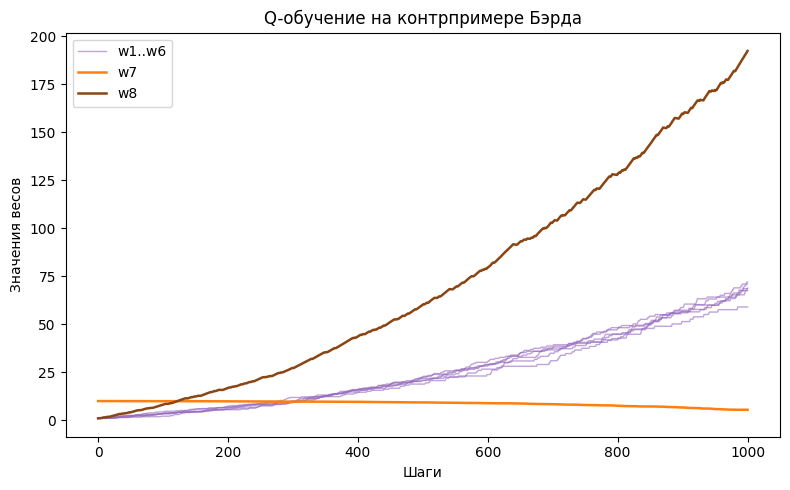
\includegraphics[width=0.8\textwidth]{fig_sol_11_3.png}
        \caption*{Эволюция весов при Q-обучении на контрпримере Бэрда.}
    \end{figure}

    Веса расходятся, как на рис.~11.2: $w_8$ взлетает (за $1000$ шагов до
    $\approx 190$, а к $5000$ шагам --- порядка $10^5$), $w_1..w_6$ растут, $w_7$
    остаётся сравнительно ограниченным. Рост неограниченный и не зависит от
    $\alpha>0$.

    Механизм --- смертельная триада. Из-за начального $w_7=10$ ценность 7-го
    состояния велика, поэтому $\max_a$ устойчиво указывает на solid, и цель всех
    обновлений бутстрапит на $\hat q(\cdot,\text{solid})=w_7+2w_8$. Обновления идут
    по off-policy распределению $b$ (в $6/7$ случаев --- на верхних состояниях, где
    dashed поднимает общий $w_8$). Но $w_8$ входит в саму цель с коэффициентом $2$,
    поэтому цель убегает вверх быстрее, чем за ней подтягиваются оценки: положительная
    обратная связь. Компенсирующих обновлений (которые вернули бы $\hat q(7)$ на
    место) поведенческая стратегия почти не даёт --- отсюда расходимость. Убрать
    любой элемент триады (аппроксимацию, бутстрэппинг или off-policy распределение)
    --- и веса сходятся.
\end{solution}
\notebook{11_03}{11.3}

\subsection{*Упражнение 11.4(с. 324)}
Докажите тождество (11.24):
\begin{equation}
    \overline{RE}(\mathbf w) = \mathbb E\big[(G_t - \hat v(S_t,\mathbf w))^2\big]
    = \overline{VE}(\mathbf w) + \mathbb E\big[(G_t - v_\pi(S_t))^2\big].
    \tag{11.24}
\end{equation}

\begin{solution}
    Обозначения: $\mathbb E[\,\cdot\mid S_t=s]$ --- усреднение по случайности дохода
    $G_t$ при фиксированном $s$; безусловное матожидание раскрывается по закону
    полного матожидания $\mathbb E[X]=\sum_s\mu(s)\,\mathbb E[X\mid S_t=s]$.
    Пользуемся тем, что при фиксированном $s$ величины $\hat v(s,\mathbf w)$ и
    $v_\pi(s)$ --- константы, а $\mathbb E[G_t\mid S_t=s]=v_\pi(s)$ по определению
    истинной ценности.

    Раскрываем $\overline{RE}$ в условное матожидание:
    \begin{equation*}
        \overline{RE}(\mathbf w) = \sum_s \mu(s)\,
        \mathbb E\big[(G_t - \hat v(s,\mathbf w))^2 \mid S_t=s\big].
    \end{equation*}
    Добавляем и вычитаем $v_\pi(s)$ и группируем:
    \begin{equation*}
        G_t - \hat v(s,\mathbf w) = \underbrace{\big(G_t - v_\pi(s)\big)}_{A}
        + \underbrace{\big(v_\pi(s) - \hat v(s,\mathbf w)\big)}_{B},
    \end{equation*}
    где при фиксированном $s$ величина $A$ случайна (зависит от $G_t$), а $B$ ---
    константа. Раскрываем квадрат под условным матожиданием:
    \begin{equation*}
        \mathbb E\big[(A+B)^2 \mid s\big]
        = \mathbb E[A^2\mid s] + 2\,\mathbb E[AB\mid s] + \mathbb E[B^2\mid s].
    \end{equation*}

    Разбираем члены. Так как $B$ --- константа при данном $s$:
    \begin{align*}
        \mathbb E[B^2\mid s] &= \big(v_\pi(s) - \hat v(s,\mathbf w)\big)^2,\\
        2\,\mathbb E[AB\mid s] &= 2B\,\mathbb E[A\mid s]
        = 2B\big(\underbrace{\mathbb E[G_t\mid S_t=s]}_{=\,v_\pi(s)} - v_\pi(s)\big) = 0.
    \end{align*}
    Перекрёстный член зануляется не из-за независимости, а потому что $B$
    выносится как константа, а $\mathbb E[A\mid s]=0$. Остаётся
    \begin{equation*}
        \mathbb E\big[(G_t - \hat v(s,\mathbf w))^2 \mid s\big]
        = \big(v_\pi(s) - \hat v(s,\mathbf w)\big)^2
        + \mathbb E\big[(G_t - v_\pi(s))^2 \mid s\big].
    \end{equation*}

    Возвращаем внешнее усреднение $\sum_s\mu(s)$:
    \begin{equation*}
        \overline{RE}(\mathbf w)
        = \underbrace{\sum_s \mu(s)\big(v_\pi(s) - \hat v(s,\mathbf w)\big)^2}_{\overline{VE}(\mathbf w)}
        + \underbrace{\sum_s \mu(s)\,\mathbb E\big[(G_t - v_\pi(s))^2\mid S_t=s\big]}_{\mathbb E[(G_t - v_\pi(S_t))^2]}.
    \end{equation*}
\end{solution}

\section{Глава 12. Следы приемлемости}

\subsection{Упражнение 12.1(с. 340)}
Доход можно выразить рекуррентно через первое вознаграждение и доход на следующем
шаге (3.9), и то же самое справедливо в отношении $\lambda$-дохода. Выведите
аналогичное рекуррентное соотношение из формул (12.2) и (12.1).
\begin{equation}
    G_{t:t+n} \doteq R_{t+1} + \gamma R_{t+2} + \dots + \gamma^{n-1} R_{t+n}
    + \gamma^n \hat v(S_{t+n}, \mathbf w_{t+n-1}), \qquad 0 \le t \le T-n.
    \tag{12.1}
\end{equation}
\begin{equation}
    G_t^\lambda \doteq (1-\lambda) \sum_{n=1}^\infty \lambda^{n-1} G_{t:t+n}.
    \tag{12.2}
\end{equation}
\begin{solution}
    Начинаем с (12.2) и отделяем член $n=1$:
    \begin{equation*}
        G_t^\lambda = (1-\lambda)\sum_{n=1}^\infty \lambda^{n-1} G_{t:t+n}
        = (1-\lambda)G_{t:t+1} + (1-\lambda)\sum_{n=2}^\infty \lambda^{n-1} G_{t:t+n}.
    \end{equation*}

    Первый член по (12.1) при $n=1$ есть $G_{t:t+1}=R_{t+1}+\gamma\hat v(S_{t+1},\mathbf w_t)$, то есть
    \begin{equation*}
        (1-\lambda)G_{t:t+1} = (1-\lambda)\big(R_{t+1}+\gamma\hat v(S_{t+1},\mathbf w_t)\big).
    \end{equation*}

    В хвосте $n\ge 2$ раскладываем $G_{t:t+n}=R_{t+1}+\gamma\,G_{t+1:t+n}$ и разбиваем на две суммы. Часть с $R_{t+1}$:
    \begin{equation*}
        (1-\lambda)R_{t+1}\sum_{n=2}^\infty \lambda^{n-1}
        = (1-\lambda)R_{t+1}\cdot\frac{\lambda}{1-\lambda} = \lambda R_{t+1}.
    \end{equation*}
    Часть с $\gamma G_{t+1:t+n}$ после сдвига $m=n-1$ сворачивается в $\lambda$-доход момента $t+1$:
    \begin{equation*}
        (1-\lambda)\gamma\sum_{n=2}^\infty \lambda^{n-1} G_{t+1:t+n}
        = \gamma\lambda\,\underbrace{(1-\lambda)\sum_{m=1}^\infty \lambda^{m-1} G_{t+1:(t+1)+m}}_{=\,G_{t+1}^\lambda}
        = \gamma\lambda\,G_{t+1}^\lambda.
    \end{equation*}

    Складываем три куска; слагаемые $(1-\lambda)R_{t+1}$ и $\lambda R_{t+1}$ дают $R_{t+1}$:
    \begin{equation*}
        G_t^\lambda = R_{t+1} + \gamma\Big[(1-\lambda)\hat v(S_{t+1},\mathbf w_t) + \lambda\,G_{t+1}^\lambda\Big].
    \end{equation*}

    Смысл рекурсии: на следующем шаге $\lambda$-доход с весом $\lambda$ продолжает
    бутстрапить дальше (через $G_{t+1}^\lambda$), а с весом $1-\lambda$
    обрывается на оценку $\hat v(S_{t+1},\mathbf w_t)$. Проверка предельными
    случаями: при $\lambda=1$ получаем $G_t^\lambda=R_{t+1}+\gamma G_{t+1}^\lambda$
    (рекурсия дохода Монте-Карло (3.9)), при $\lambda=0$ ---
    $G_t^\lambda=R_{t+1}+\gamma\hat v(S_{t+1},\mathbf w_t)$ (одношаговый TD-таргет).
\end{solution}

\subsection{Упражнение 12.2(с. 340)}
Параметр $\lambda$ характеризует скорость экспоненциального убывания весов на
рис.~2.2, а значит, то, насколько далеко в будущее заглядывает $\lambda$-доходный
алгоритм при вычислении обновления. Но коэффициенты типа $\lambda$ --- не всегда
удачный способ описать скорость убывания. Иногда лучше задавать временную
постоянную, или время полужизни. Напишите уравнение, связывающее $\lambda$ и время
полужизни $T_\lambda$, т.\,е. время, за которое вес снизится до половины
начального значения.

\begin{solution}
    Веса $n$-шаговых доходов в $\lambda$-доходе суть $w_n=(1-\lambda)\lambda^{n-1}$;
    экспоненциально убывающая часть --- $\lambda^{n-1}$ (общий множитель $1-\lambda$
    в отношении сократится). Моделируя вес непрерывно как $\lambda^{\tau}$,
    определяем полужизнь $T_\lambda$ из условия «вес упал вдвое»:
    \begin{equation*}
        \lambda^{T_\lambda} = \tfrac12.
    \end{equation*}
    Логарифмируя обе части и переходя к натуральному логарифму:
    \begin{equation*}
        T_\lambda = -\log_\lambda 2 = -\frac{\ln 2}{\ln\lambda} = \frac{\ln 2}{\ln(1/\lambda)}.
    \end{equation*}
    Последняя запись нагляднее: при $\lambda\in(0,1)$ знаменатель $\ln(1/\lambda)>0$,
    поэтому $T_\lambda>0$.

    Проверка предельными случаями: при $\lambda\to 1^-$ имеем $T_\lambda\to+\infty$
    (Монте-Карло, доход заглядывает бесконечно далеко), при $\lambda\to 0^+$ ---
    $T_\lambda\to 0$ (одношаговый TD, заглядывания вперёд почти нет).
\end{solution}

\subsection{Упражнение 12.3(с. 346)}
Получить более полное представление о том, насколько хорошо TD($\lambda$) может
аппроксимировать офлайновый $\lambda$-доходный алгоритм, можно, заметив, что член
ошибки в последнем (выражение в квадратных скобках в (12.4)) можно записать в
виде суммы TD-ошибок (12.6) для одного фиксированного $\mathbf w$. Докажите это,
следуя образцу (6.6) и воспользовавшись рекуррентным соотношением для
$\lambda$-дохода, которое вы вывели, решая упражнение 12.1.

Офлайновый $\lambda$-доходный алгоритм (12.4):
\begin{equation}
    \mathbf w_{t+1} \doteq \mathbf w_t + \alpha\big[G_t^\lambda - \hat v(S_t,\mathbf w_t)\big]\nabla\hat v(S_t,\mathbf w_t),
    \qquad t = 0,\dots,T-1.
    \tag{12.4}
\end{equation}
TD-ошибка (12.6):
\begin{equation}
    \delta_t \doteq R_{t+1} + \gamma\hat v(S_{t+1},\mathbf w_t) - \hat v(S_t,\mathbf w_t).
    \tag{12.6}
\end{equation}
Образец --- табличное тождество (6.6):
\begin{equation}
    G_t - V(S_t) = \sum_{k=t}^{T-1} \gamma^{k-t}\,\delta_k.
    \tag{6.6}
\end{equation}
Рекуррентное соотношение для $\lambda$-дохода (из упражнения 12.1):
\begin{equation*}
    G_t^\lambda = R_{t+1} + \gamma(1-\lambda)\hat v(S_{t+1},\mathbf w) + \gamma\lambda\,G_{t+1}^\lambda.
\end{equation*}

\begin{solution}
    Веса фиксированы, поэтому пишем $\hat v(\cdot)$ без индекса шага, а $\delta_k =
    R_{k+1}+\gamma\hat v(S_{k+1})-\hat v(S_k)$. Обозначим член ошибки $E_t \doteq
    G_t^\lambda - \hat v(S_t)$.

    Вычитаем $\hat v(S_t)$ из рекурсии $\lambda$-дохода:
    \begin{equation*}
        E_t = R_{t+1} + \gamma(1-\lambda)\hat v(S_{t+1}) - \hat v(S_t) + \gamma\lambda\,G_{t+1}^\lambda.
    \end{equation*}
    По образцу (6.6) добавляем и вычитаем $\gamma\lambda\hat v(S_{t+1})$, чтобы
    выделить TD-ошибку. Используем $\gamma(1-\lambda)\hat v(S_{t+1}) = \gamma\hat
    v(S_{t+1}) - \gamma\lambda\hat v(S_{t+1})$:
    \begin{equation*}
        R_{t+1} + \gamma(1-\lambda)\hat v(S_{t+1}) - \hat v(S_t)
        = \underbrace{R_{t+1} + \gamma\hat v(S_{t+1}) - \hat v(S_t)}_{\delta_t}
          - \gamma\lambda\hat v(S_{t+1}).
    \end{equation*}
    Подставляя обратно и группируя, получаем рекурсию для ошибки:
    \begin{equation*}
        E_t = \delta_t + \gamma\lambda\big(G_{t+1}^\lambda - \hat v(S_{t+1})\big)
        = \delta_t + \gamma\lambda\,E_{t+1}.
    \end{equation*}
    Раскручивая её (как в (6.6)) и учитывая, что в конце эпизода $E_T=0$, а
    $\delta_k=0$ при $k\ge T$:
    \begin{equation*}
        E_t = \delta_t + \gamma\lambda\,\delta_{t+1} + (\gamma\lambda)^2\delta_{t+2} + \dots
        = \sum_{k=t}^{T-1} (\gamma\lambda)^{k-t}\,\delta_k.
    \end{equation*}
    То есть
    \begin{equation*}
        G_t^\lambda - \hat v(S_t) = \sum_{k=t}^{T-1} (\gamma\lambda)^{k-t}\,\delta_k.
    \end{equation*}

    Два замечания. Тождество держится только при фиксированном $\mathbf w$: иначе
    $\delta_k$ считались бы через разные $\mathbf w_k$, добавленное и вычтенное
    $\hat v(S_{t+1})$ не сократились бы. Именно поэтому TD($\lambda$) лишь
    приближает офлайновый $\lambda$-доход --- онлайн $\mathbf w$ меняется внутри
    эпизода. В отличие от (6.6) множитель здесь $(\gamma\lambda)^{k-t}$, а не
    $\gamma^{k-t}$: лишний $\lambda$ приходит из коэффициента $\gamma\lambda$ при
    рекурсивном члене --- тот же темп затухания, что у следа приемлемости
    $\mathbf z_t$.
\end{solution}

\subsection{Упражнение 12.4(с. 346)}
Воспользуйтесь результатом предыдущего упражнения, чтобы показать, что если бы
обновления весов в эпизоде вычислялись на каждом шаге, но не использовались для
изменения весов ($\mathbf w$ оставался бы фиксированным), то сумма обновлений
весов в TD($\lambda$) была бы такой же, как сумма обновлений в офлайновом
$\lambda$-доходном алгоритме.

\begin{solution}
    Веса фиксированы, шаг $\alpha$ вынесем. Надо показать равенство суммарных
    обновлений за эпизод.

    Офлайновый $\lambda$-доход (12.4), с подстановкой результата упражнения 12.3
    $G_t^\lambda-\hat v(S_t)=\sum_{k=t}^{T-1}(\gamma\lambda)^{k-t}\delta_k$:
    \begin{equation*}
        \mathrm{L} = \sum_{t=0}^{T-1}\alpha\big[G_t^\lambda-\hat v(S_t)\big]\nabla\hat v(S_t)
        = \alpha\sum_{t=0}^{T-1}\sum_{k=t}^{T-1}(\gamma\lambda)^{k-t}\,\delta_k\,\nabla\hat v(S_t).
    \end{equation*}

    TD($\lambda$) (12.7) со следом (12.5), развёрнутым как $\mathbf z_t=\sum_{k=0}^{t}(\gamma\lambda)^{t-k}\nabla\hat v(S_k)$:
    \begin{equation*}
        \mathrm{R} = \sum_{t=0}^{T-1}\alpha\,\delta_t\,\mathbf z_t
        = \alpha\sum_{t=0}^{T-1}\sum_{k=0}^{t}(\gamma\lambda)^{t-k}\,\delta_t\,\nabla\hat v(S_k).
    \end{equation*}

    В $\mathrm{R}$ переименуем индексы $t\leftrightarrow k$ (внешний назовём $k$, внутренний $t$):
    \begin{equation*}
        \mathrm{R} = \alpha\sum_{k=0}^{T-1}\sum_{t=0}^{k}(\gamma\lambda)^{k-t}\,\delta_k\,\nabla\hat v(S_t).
    \end{equation*}
    Теперь обе суммы идут по одному треугольному множеству индексов
    $\{(t,k):0\le t\le k\le T-1\}$ с одинаковым слагаемым $(\gamma\lambda)^{k-t}\delta_k\nabla\hat v(S_t)$.
    $\mathrm{L}$ суммирует его по строкам (фиксирован $t$, бежит $k\ge t$), $\mathrm{R}$ ---
    по столбцам (фиксирован $k$, бежит $t\le k$); сумма всех элементов одна, поэтому
    \begin{equation*}
        \mathrm{L} = \mathrm{R},
    \end{equation*}
    то есть суммарные обновления совпадают.

    Всё держится на фиксированном $\mathbf w$: иначе $\delta_k$ и $\nabla\hat v$ на
    разных шагах вычислялись бы через разные $\mathbf w_t$, слагаемые не совпали бы,
    и перестановка порядка суммирования не дала бы тождества. Поэтому равенство
    суммарных обновлений точное лишь при неизменных весах --- при онлайновом
    изменении $\mathbf w$ TD($\lambda$) только приближает офлайновый
    $\lambda$-доходный алгоритм.
\end{solution}

\subsection{Упражнение 12.5(с. 347)}
Мы уже несколько раз (часто в упражнениях) устанавливали, что доход можно
записать в виде суммы TD-ошибок, если функция ценности остаётся постоянной.
Почему (12.10) является ещё одним примером такого рода? Докажите тождество
(12.10).

Усечённый $\lambda$-доход (12.10) с TD-ошибкой
\begin{equation}
    G_{t:t+k}^\lambda = \hat v(S_t,\mathbf w_{t-1})
    + \sum_{i=t}^{t+k-1} (\gamma\lambda)^{i-t}\,\delta_i',
    \qquad
    \delta_i' \doteq R_{i+1} + \gamma\hat v(S_{i+1},\mathbf w_i) - \hat v(S_i,\mathbf w_{i-1}).
    \tag{12.10}
\end{equation}

\begin{solution}
    Обозначим ошибку $E_{t:t+k}\doteq G_{t:t+k}^\lambda - \hat v(S_t,\mathbf w_{t-1})$.

    Усечённый $\lambda$-доход подчиняется той же рекурсии, что и в упражнении 12.1,
    с укороченным на шаг горизонтом:
    \begin{equation*}
        G_{t:t+k}^\lambda = R_{t+1} + \gamma(1-\lambda)\hat v(S_{t+1},\mathbf w_t)
        + \gamma\lambda\,G_{t+1:t+k}^\lambda.
    \end{equation*}
    Вычитаем $\hat v(S_t,\mathbf w_{t-1})$ и расщепляем $\gamma\hat v(S_{t+1},\mathbf w_t)
    = \gamma\lambda\hat v(S_{t+1},\mathbf w_t) + \gamma(1-\lambda)\hat v(S_{t+1},\mathbf w_t)$,
    чтобы выделить $\delta_t'$:
    \begin{equation*}
        R_{t+1} + \gamma(1-\lambda)\hat v(S_{t+1},\mathbf w_t) - \hat v(S_t,\mathbf w_{t-1})
        = \underbrace{R_{t+1} + \gamma\hat v(S_{t+1},\mathbf w_t) - \hat v(S_t,\mathbf w_{t-1})}_{\delta_t'}
          - \gamma\lambda\hat v(S_{t+1},\mathbf w_t).
    \end{equation*}
    Подставляя, получаем рекурсию для ошибки:
    \begin{equation*}
        E_{t:t+k} = \delta_t' + \gamma\lambda\big(G_{t+1:t+k}^\lambda - \hat v(S_{t+1},\mathbf w_t)\big)
        = \delta_t' + \gamma\lambda\,E_{t+1:t+k}.
    \end{equation*}
    Вычитаемое $\hat v(S_{t+1},\mathbf w_t)$ имеет ровно тот индекс весов, что и в
    определении $E_{t+1:t+k}$, так что члены согласованы. База рекурсии:
    $E_{t+k:t+k}=0$ (усечённый доход нулевой длины равен бутстрапу $\hat
    v(S_{t+k},\mathbf w_{t+k-1})$). Раскручивая:
    \begin{equation*}
        E_{t:t+k} = \sum_{i=t}^{t+k-1} (\gamma\lambda)^{i-t}\,\delta_i',
        \qquad\text{откуда}\qquad
        G_{t:t+k}^\lambda = \hat v(S_t,\mathbf w_{t-1}) + \sum_{i=t}^{t+k-1} (\gamma\lambda)^{i-t}\,\delta_i'.
    \end{equation*}
\end{solution}

\subsection{Упражнение 12.6(с. 357)}
Модифицируйте псевдокод алгоритма Sarsa($\lambda$) так, чтобы использовать
голландские следы (12.11) и никаких других особенностей истинно онлайнового
алгоритма. Предполагайте, что аппроксимация функций линейна, а признаки бинарны.
\begin{equation}
    \mathbf z_t \doteq \gamma\lambda\,\mathbf z_{t-1}
    + \big(1 - \alpha\gamma\lambda\,\mathbf z_{t-1}^\top \mathbf x_t\big)\mathbf x_t,
    \tag{12.11}
\end{equation}
\begin{solution}
    Истинно онлайновый Sarsa($\lambda$) отличается от обычного двумя неразрывными
    элементами: голландским следом (12.11) вместо накопительного/замещающего и
    поправкой на изменение оценки текущего действия через $Q_{old}$ (оценку
    выбранного действия по весам \emph{до} их обновления). Для бинарных признаков
    $\mathbf w^\top\mathbf x = \sum_{i\in\mathcal F(S,A)} w_i$ и $\mathbf z^\top\mathbf x
    = \sum_{i\in\mathcal F(S,A)} z_i$.

    \begin{algorithm}[H]
        \DontPrintSemicolon
        \SetKwInOut{Input}{Вход}
        \SetKwInOut{Param}{Параметры}
        \Input{функция $\mathcal F(s,a)$ (индексы активных признаков); стратегия $\pi$ (если оценивается $q_\pi$)}
        \Param{размер шага $\alpha>0$, скорость затухания следа $\lambda\in[0,1]$}
        Инициализировать $\mathbf w\in\mathbb R^d$ произвольно (например, $\mathbf w=\mathbf 0$)\;
        \For{\textnormal{каждого эпизода}}{
            Инициализировать $S$; выбрать $A\sim\pi(\cdot\mid S)$ или $\varepsilon$-жадно по $\hat q(S,\cdot,\mathbf w)$\;
            $\mathbf x\leftarrow \mathbf x(S,A)$ \tcp*{бинарный вектор признаков пары $(S,A)$}
            $\mathbf z\leftarrow \mathbf 0$;\quad $Q_{old}\leftarrow 0$\;
            \Repeat{$S'$ \textnormal{заключительное}}{
                Предпринять действие $A$; наблюдать $R,S'$\;
                Выбрать $A'\sim\pi(\cdot\mid S')$ или $\varepsilon$-жадно по $\hat q(S',\cdot,\mathbf w)$\;
                $\mathbf x'\leftarrow \mathbf x(S',A')$ \tcp*{$\mathbf 0$, если $S'$ заключительное}
                $Q\leftarrow \mathbf w^\top\mathbf x$;\quad $Q'\leftarrow \mathbf w^\top\mathbf x'$\;
                $\delta\leftarrow R+\gamma Q'-Q$\;
                $\mathbf z\leftarrow \gamma\lambda\,\mathbf z+\big(1-\alpha\gamma\lambda\,\mathbf z^\top\mathbf x\big)\mathbf x$ \tcp*{голландский след (12.11)}
                $\mathbf w\leftarrow \mathbf w+\alpha(\delta+Q-Q_{old})\,\mathbf z-\alpha(Q-Q_{old})\,\mathbf x$\;
                $Q_{old}\leftarrow Q'$\;
                $\mathbf x\leftarrow \mathbf x'$;\quad $A\leftarrow A'$\;
            }
        }
    \end{algorithm}

    Пояснения. Скаляр $\mathbf z^\top\mathbf x$ в строке следа вычисляется по $\mathbf z$
    \emph{до} присваивания (роль $\mathbf z_{t-1}$), а затухание $\gamma\lambda$
    включено в ту же строку --- поэтому оба множителя $\gamma\lambda$ стоят явно, и
    отдельной строки затухания в конце шага нет. Обновление весов эквивалентно
    $\mathbf w\leftarrow \mathbf w+\alpha\delta\mathbf z+\alpha(Q-Q_{old})(\mathbf z-\mathbf x)$:
    первый член --- как в обычном Sarsa($\lambda$), второй компенсирует изменение
    оценки текущего действия за такт. $Q_{old}$ хранит оценку выбранного действия
    $A'$ (которое станет текущим на следующем шаге), снятую по весам до их
    обновления. Для бинарных признаков произведения $\mathbf w^\top\mathbf x$,
    $\mathbf w^\top\mathbf x'$, $\mathbf z^\top\mathbf x$ --- это суммы соответствующих
    компонент по активным индексам из $\mathcal F$.
\end{solution}

\subsection{Упражнение 12.7(с. 360)}
Обобщите все три приведённых выше рекуррентных соотношения на усечённые версии,
определив $G_{t:h}^{\lambda s}$ и $G_{t:h}^{\lambda a}$.

\begin{solution}
    В каждую из рекурсий (12.18)--(12.20) добавляем горизонт усечения $h$ (как
    (12.9) к обычному $\lambda$-доходу): вложенный доход становится усечённым тем
    же горизонтом, а на $t=h$ рекурсия обрывается на бутстрап-оценку (переменные
    $\lambda_{t+1}$ и $\gamma_{t+1}$ сохраняются).

    Доход для состояний:
    \begin{align*}
        G_{t:h}^{\lambda s} &\doteq R_{t+1} + \gamma_{t+1}\Big((1-\lambda_{t+1})\hat v(S_{t+1},\mathbf w_t) + \lambda_{t+1}\,G_{t+1:h}^{\lambda s}\Big), \qquad t<h,\\
        G_{h:h}^{\lambda s} &\doteq \hat v(S_h,\mathbf w_{h-1}).
    \end{align*}

    Доход для действий (Sarsa) --- $\hat q$ вместо $\hat v$:
    \begin{align*}
        G_{t:h}^{\lambda a} &\doteq R_{t+1} + \gamma_{t+1}\Big((1-\lambda_{t+1})\hat q(S_{t+1},A_{t+1},\mathbf w_t) + \lambda_{t+1}\,G_{t+1:h}^{\lambda a}\Big), \qquad t<h,\\
        G_{h:h}^{\lambda a} &\doteq \hat q(S_h,A_h,\mathbf w_{h-1}).
    \end{align*}

    Доход для действий (Expected Sarsa) --- бутстрап через ожидание $\bar V_t(S_{t+1})=\sum_a \pi(a\mid S_{t+1})\hat q(S_{t+1},a,\mathbf w_t)$:
    \begin{align*}
        G_{t:h}^{\lambda a} &\doteq R_{t+1} + \gamma_{t+1}\Big((1-\lambda_{t+1})\bar V_t(S_{t+1}) + \lambda_{t+1}\,G_{t+1:h}^{\lambda a}\Big), \qquad t<h,\\
        G_{h:h}^{\lambda a} &\doteq \bar V_{h-1}(S_h).
    \end{align*}

    Проверка: при $h=t+1$ каждая рекурсия сворачивается в соответствующий
    одношаговый таргет ($R_{t+1}+\gamma_{t+1}\hat v(S_{t+1},\mathbf w_t)$ и
    аналогично для $\hat q$, $\bar V$) независимо от $\lambda_{t+1}$.
\end{solution}

\subsection{Упражнение 12.8(с. 361)}
Докажите, что приближённое равенство (12.24) становится точным, если функция
ценности не изменяется. Для сокращения записи рассмотрите случай $t=0$ и
воспользуйтесь нотацией $V_k \doteq \hat v(S_k,\mathbf w)$.
\begin{equation}
    G_0^{\lambda s} - V_0 = \sum_{k=0}^{\infty}\Big(\prod_{i=1}^{k}\gamma_i\lambda_i\rho_i\Big)\rho_k\,\delta_k^s,
    \qquad \delta_k^s = R_{k+1} + \gamma_{k+1}V_{k+1} - V_k.
    \tag{12.24}
\end{equation}
\begin{solution}
    Веса фиксированы, поэтому $V_k=\hat v(S_k,\mathbf w)$ и $\delta_k^s$ не зависят
    от шага обновления. Обозначим $E_t \doteq G_t^{\lambda s} - V_t$.

    Берём (12.22) и вычитаем $V_t$. Член $(1-\rho_t)V_t$ вместе с $-V_t$ даёт
    $-\rho_t V_t$, поэтому
    \begin{equation*}
        E_t = \rho_t\big(R_{t+1} + \gamma_{t+1}((1-\lambda_{t+1})V_{t+1} + \lambda_{t+1}G_{t+1}^{\lambda s})\big) - \rho_t V_t.
    \end{equation*}
    Расщепляем $\gamma_{t+1}V_{t+1} = \gamma_{t+1}\lambda_{t+1}V_{t+1} + \gamma_{t+1}(1-\lambda_{t+1})V_{t+1}$,
    чтобы выделить $\delta_t^s$:
    \begin{equation*}
        R_{t+1} + \gamma_{t+1}(1-\lambda_{t+1})V_{t+1} - V_t
        = \underbrace{R_{t+1} + \gamma_{t+1}V_{t+1} - V_t}_{\delta_t^s} - \gamma_{t+1}\lambda_{t+1}V_{t+1}.
    \end{equation*}
    Подставляя, получаем рекурсию для ошибки:
    \begin{equation*}
        E_t = \rho_t\,\delta_t^s + \rho_t\gamma_{t+1}\lambda_{t+1}\big(G_{t+1}^{\lambda s} - V_{t+1}\big)
        = \rho_t\,\delta_t^s + \rho_t\gamma_{t+1}\lambda_{t+1}\,E_{t+1}.
    \end{equation*}

    Раскручиваем от $t=0$. Каждый шаг вносит множитель $\rho_t\gamma_{t+1}\lambda_{t+1}$,
    а в самом $E_{t+1}$ перед $\delta_{t+1}^s$ стоит свой $\rho_{t+1}$:
    \begin{align*}
        E_0 &= \rho_0\delta_0^s + \rho_0\gamma_1\lambda_1 E_1
             = \rho_0\delta_0^s + \rho_0\gamma_1\lambda_1\big(\rho_1\delta_1^s + \rho_1\gamma_2\lambda_2 E_2\big)\\
            &= \rho_0\delta_0^s + \gamma_1\lambda_1\rho_1\,\rho_1... \quad\Longrightarrow\quad
            E_0 = \sum_{k=0}^{\infty}\Big(\prod_{i=1}^{k}\gamma_i\lambda_i\rho_i\Big)\rho_k\,\delta_k^s.
    \end{align*}
    Множитель $\rho_k$ снаружи произведения приходит из самого $E_k$, а
    $\prod_{i=1}^{k}\gamma_i\lambda_i\rho_i$ --- из накопленных рекурсивных
    коэффициентов. Итого
    \begin{equation*}
        G_0^{\lambda s} - V_0 = \sum_{k=0}^{\infty}\Big(\prod_{i=1}^{k}\gamma_i\lambda_i\rho_i\Big)\rho_k\,\delta_k^s.
    \end{equation*}

    Равенство точное лишь при неизменных весах: только тогда все $V_k$ и
    $\delta_k^s$ считаются через один $\mathbf w$ и добавленные-вычтенные $V_{t+1}$
    сокращаются в телескопе.
\end{solution}

\subsection{Упражнение 12.9(с. 361)}
Усечённый вариант общего дохода с разделённой стратегией обозначается
$G_{t:h}^{\lambda s}$. Попробуйте угадать его правильное выражение, взяв за основу
(12.24).

\begin{solution}
    По образцу (12.24) усечение горизонтом $h$ означает, что доступны только
    TD-ошибки $\delta_k^s$ до $k=h-1$ (последняя, $\delta_{h-1}^s$, бутстрапит на
    $V_h$). Обобщая (12.24) с произвольного $t$ и обрезая сумму на $h-1$:
    \begin{equation*}
        G_{t:h}^{\lambda s} = V_t + \sum_{k=t}^{h-1}\Big(\prod_{i=t+1}^{k}\gamma_i\lambda_i\rho_i\Big)\rho_k\,\delta_k^s,
    \end{equation*}
    где $V_k = \hat v(S_k,\mathbf w)$, $\delta_k^s = R_{k+1} + \gamma_{k+1}V_{k+1} - V_k$,
    а $\rho_k = \pi(A_k\mid S_k)/b(A_k\mid S_k)$. При $k=t$ произведение пустое и
    равно $1$, так что первый член суммы --- $\rho_t\delta_t^s$.

    Проверки. Крайний член $\delta_{h-1}^s$ вносит $\gamma_h V_h$, то есть доход
    упирается в бутстрап $\hat v(S_h,\mathbf w)$ на горизонте --- согласуется с
    базой рекурсии из упражнения 12.7 ($G_{h:h}^{\lambda s}=\hat v(S_h)$). При
    $h\to\infty$ выражение переходит в неусечённое (12.24).

    Замечание. Как и (12.24), это выражение точно при неизменных весах (все $V_k$
    считаются через один $\mathbf w$). В онлайновом использовании веса меняются, и
    строгая форма потребовала бы переиндексации весов внутри $\delta_k^s$ (как
    $\delta_i'$ с $\mathbf w_i,\mathbf w_{i-1}$ в (12.10)); но по образцу (12.24)
    достаточно приведённой формы.
\end{solution}

\subsection{Упражнение 12.10(с. 363)}
Докажите, что приближённое равенство (12.27) становится точным, если функция
ценности не изменяется. Для сокращения записи рассмотрите случай $t=0$ и
воспользуйтесь нотацией $Q_k \doteq \hat q(S_k,A_k,\mathbf w)$.

\begin{equation}
    G_0^{\lambda a} - Q_0 = \sum_{k=0}^{\infty}\Big(\prod_{i=1}^{k}\gamma_i\lambda_i\rho_i\Big)\delta_k^a,
    \qquad \delta_k^a = R_{k+1} + \gamma_{k+1}\bar V_k(S_{k+1}) - Q_k,
    \tag{12.27}
\end{equation}
где $\bar V_k(S_{k+1}) = \sum_a \pi(a\mid S_{k+1})\hat q(S_{k+1},a,\mathbf w)$.

\begin{solution}
    Веса фиксированы, $Q_k=\hat q(S_k,A_k,\mathbf w)$. Обозначим $E_t \doteq
    G_t^{\lambda a} - Q_t$. Off-policy $\lambda$-доход Expected Sarsa (12.26) ---
    текущее действие усредняется ожиданием $\bar V_t$, а importance sampling
    $\rho_{t+1}$ корректирует лишь переход к следующему доходу:
    \begin{equation*}
        G_t^{\lambda a} = R_{t+1} + \gamma_{t+1}\Big[(1-\lambda_{t+1})\bar V_t(S_{t+1})
        + \lambda_{t+1}\big(\rho_{t+1}G_{t+1}^{\lambda a} + (1-\rho_{t+1})\bar V_t(S_{t+1})\big)\Big].
    \end{equation*}

    Вычитаем $Q_0$ (берём $t=0$). Слагаемые с $\bar V_0(S_1)$ собираются как
    $\gamma_1(1-\lambda_1)\bar V_0 + \gamma_1\lambda_1(1-\rho_1)\bar V_0
    = \gamma_1\bar V_0 - \gamma_1\lambda_1\rho_1\bar V_0$, поэтому
    \begin{equation*}
        E_0 = \underbrace{R_1 + \gamma_1\bar V_0(S_1) - Q_0}_{\delta_0^a}
        + \gamma_1\lambda_1\rho_1\big(G_1^{\lambda a} - \bar V_0(S_1)\big).
    \end{equation*}
    Замена $\bar V_0(S_1)\to Q_1$ в последнем члене компенсируется определением
    $\delta_1^a$ на следующем шаге (бутстрап через $\bar V_1$), что даёт чистую
    рекурсию
    \begin{equation*}
        E_0 = \delta_0^a + \gamma_1\lambda_1\rho_1\,E_1.
    \end{equation*}
    В общем виде $E_t = \delta_t^a + \gamma_{t+1}\lambda_{t+1}\rho_{t+1}E_{t+1}$.
    Раскручивая от $t=0$:
    \begin{equation*}
        G_0^{\lambda a} - Q_0 = \sum_{k=0}^{\infty}\Big(\prod_{i=1}^{k}\gamma_i\lambda_i\rho_i\Big)\delta_k^a.
    \end{equation*}
\end{solution}

\subsection{Упражнение 12.11(с. 363)}
Усечённый вариант общего дохода с разделённой стратегией обозначается
$G_{t:h}^{\lambda a}$. Попробуйте угадать его правильное выражение, взяв за основу
(12.27).

\begin{solution}
    По образцу (12.27) усечение горизонтом $h$ обрезает сумму на $k=h-1$
    (последняя ошибка $\delta_{h-1}^a$ бутстрапит на шаг $h$):
    \begin{equation*}
        G_{t:h}^{\lambda a} = Q_t + \sum_{k=t}^{h-1}\Big(\prod_{i=t+1}^{k}\gamma_i\lambda_i\rho_i\Big)\delta_k^a,
    \end{equation*}
    где $Q_k = \hat q(S_k,A_k,\mathbf w)$, $\delta_k^a = R_{k+1} + \gamma_{k+1}\bar V_k(S_{k+1}) - Q_k$,
    $\bar V_k(S_{k+1}) = \sum_a \pi(a\mid S_{k+1})\hat q(S_{k+1},a,\mathbf w)$, а
    $\rho_i = \pi(A_i\mid S_i)/b(A_i\mid S_i)$. При $k=t$ произведение пустое ($=1$),
    так что первый член суммы --- просто $\delta_t^a$.

    Проверки. Как и в (12.27), снаружи произведения \emph{нет} отдельного
    множителя $\rho_k$ (в отличие от усечённого дохода для состояний из
    упражнения 12.9) --- текущее действие усредняется через $\bar V_k$, поэтому
    $\rho$ входит лишь за переходы. Крайний член $\delta_{h-1}^a$ вносит
    $\gamma_h\bar V_{h-1}(S_h)$, то есть доход упирается в ожидание $\bar
    V_{h-1}(S_h)$ на горизонте --- согласуется с базой Expected Sarsa из упражнения
    12.7 ($G_{h:h}^{\lambda a}=\bar V_{h-1}(S_h)$). При $h\to\infty$ выражение
    переходит в неусечённое (12.27).
\end{solution}

\subsection{Упражнение 12.12(с. 363)}
Детально проведите все намеченные выше шаги вывода (12.29) из (12.27). Начните с
обновления (12.15), подставьте $G_t^{\lambda a}$ из (12.26) вместо $G_t^\lambda$, а
затем выполните те же шаги, что привели к (12.25).
\begin{equation}
    \mathbf w_{t+1} \doteq \mathbf w_t + \alpha\big[G_t^\lambda - \hat q(S_t,A_t,\mathbf w_t)\big]\nabla\hat q(S_t,A_t,\mathbf w_t).
    \tag{12.15}
\end{equation}
\begin{equation}
    G_t^{\lambda a} \doteq R_{t+1} + \gamma_{t+1}\Big[(1-\lambda_{t+1})\bar V_t(S_{t+1})
    + \lambda_{t+1}\big(\rho_{t+1}G_{t+1}^{\lambda a} + (1-\rho_{t+1})\bar V_t(S_{t+1})\big)\Big].
    \tag{12.26}
\end{equation}
\begin{equation}
    G_t^{\lambda a} - \hat q(S_t,A_t,\mathbf w) \approx
    \sum_{k=t}^{\infty}\Big(\prod_{i=t+1}^{k}\gamma_i\lambda_i\rho_i\Big)\delta_k^a.
    \tag{12.27}
\end{equation}
\begin{equation}
    \mathbf z_t \doteq \gamma_t\lambda_t\rho_t\,\mathbf z_{t-1} + \rho_t\nabla\hat v(S_t,\mathbf w_t).
    \tag{12.25}
\end{equation}
\begin{equation}
    \mathbf z_t \doteq \gamma_t\lambda_t\rho_t\,\mathbf z_{t-1} + \nabla\hat q(S_t,A_t,\mathbf w_t).
    \tag{12.29}
\end{equation}
\begin{solution}
    Веса считаем фиксированными (при этом (12.27) точно), обозначим
    $\nabla_t \doteq \nabla\hat q(S_t,A_t,\mathbf w_t)$, $Q_t=\hat q(S_t,A_t,\mathbf w_t)$.

    Обновление прямого представления (12.15) с $\lambda$-доходом для действий:
    \begin{equation*}
        \mathbf w_{t+1} = \mathbf w_t + \alpha\big[G_t^{\lambda a} - Q_t\big]\nabla_t.
    \end{equation*}
    Подставляем разложение (12.27), $G_t^{\lambda a}-Q_t=\sum_{k=t}^{\infty}
    \big(\prod_{i=t+1}^{k}\gamma_i\lambda_i\rho_i\big)\delta_k^a$, и суммируем
    обновления:
    \begin{equation*}
        \sum_{t}\Delta\mathbf w_t
        = \alpha\sum_{t=0}^{\infty}\sum_{k=t}^{\infty}
          \Big(\prod_{i=t+1}^{k}\gamma_i\lambda_i\rho_i\Big)\delta_k^a\,\nabla_t.
    \end{equation*}

    Применяем правило суммирования (меняем порядок обхода треугольника $t\le k$,
    как в упражнении 12.4):
    \begin{equation*}
        = \alpha\sum_{k=0}^{\infty}\delta_k^a
          \underbrace{\sum_{t=0}^{k}\Big(\prod_{i=t+1}^{k}\gamma_i\lambda_i\rho_i\Big)\nabla_t}_{\displaystyle \doteq\ \mathbf z_k},
    \end{equation*}
    то есть обновление приобретает обычную полуградиентную форму (12.7)
    $\mathbf w \leftarrow \mathbf w + \alpha\delta_k^a\mathbf z_k$, где $\mathbf z_k$ ---
    внутренняя сумма.

    Выведем для неё рекурсию. Отделяем член $t=k$ (произведение пустое, равно $1$) и
    выносим из остальных общий множитель с $i=k$, пользуясь
    $\prod_{i=t+1}^{k}\gamma_i\lambda_i\rho_i = \gamma_k\lambda_k\rho_k\prod_{i=t+1}^{k-1}\gamma_i\lambda_i\rho_i$:
    \begin{equation*}
        \mathbf z_k = \nabla_k + \gamma_k\lambda_k\rho_k
        \underbrace{\sum_{t=0}^{k-1}\Big(\prod_{i=t+1}^{k-1}\gamma_i\lambda_i\rho_i\Big)\nabla_t}_{=\ \mathbf z_{k-1}}
        = \gamma_k\lambda_k\rho_k\,\mathbf z_{k-1} + \nabla_k.
    \end{equation*}
    Переименовав $k\to t$, получаем (12.29):
    \begin{equation*}
        \mathbf z_t \doteq \gamma_t\lambda_t\rho_t\,\mathbf z_{t-1} + \nabla\hat q(S_t,A_t,\mathbf w_t).
    \end{equation*}
\end{solution}

\subsection{Упражнение 12.13(с. 364)}
Как выглядят «голландский» и «замещающий» варианты следов приемлемости с
разделённой стратегией для методов вычисления ценности состояний и действий?

\begin{solution}
    Отправная точка --- накопительные следы с разделённой стратегией: (12.25) для
    состояний и (12.29) для действий. Модифицируется только способ добавления
    свежего вклада; член переноса $\gamma_t\lambda_t\rho_t\mathbf z_{t-1}$ во всех
    вариантах одинаков. Замещающие следы определены для бинарных признаков.

    \textbf{Ценности состояний.} Свежий вклад входит с множителем $\rho_t$.
    \begin{align*}
        \text{накопительный:}\quad
        &\mathbf z_t = \gamma_t\lambda_t\rho_t\,\mathbf z_{t-1} + \rho_t\nabla\hat v(S_t,\mathbf w_t),\\
        \text{замещающий:}\quad
        &z_{i,t} =
        \begin{cases}
            \rho_t, & x_i(S_t) = 1,\\
            \gamma_t\lambda_t\rho_t\,z_{i,t-1}, & \text{иначе},
        \end{cases}\\
        \text{голландский:}\quad
        &\mathbf z_t = \gamma_t\lambda_t\rho_t\,\mathbf z_{t-1}
        + \rho_t\big(1 - \alpha\gamma_t\lambda_t\rho_t\,\mathbf z_{t-1}^\top\mathbf x_t\big)\mathbf x_t,
        \quad \mathbf x_t = \mathbf x(S_t).
    \end{align*}
    В замещающем варианте активные компоненты сбрасываются в $\rho_t$, а не в
    единицу: при $\rho_t=0$ (целевая стратегия никогда не выбрала бы это действие)
    след обязан обнулиться полностью.

    \textbf{Ценности действий.} Свежий вклад входит без множителя $\rho_t$.
    \begin{align*}
        \text{накопительный:}\quad
        &\mathbf z_t = \gamma_t\lambda_t\rho_t\,\mathbf z_{t-1} + \nabla\hat q(S_t,A_t,\mathbf w_t),\\
        \text{замещающий:}\quad
        &z_{i,t} =
        \begin{cases}
            1, & x_i(S_t,A_t) = 1,\\
            \gamma_t\lambda_t\rho_t\,z_{i,t-1}, & \text{иначе},
        \end{cases}\\
        \text{голландский:}\quad
        &\mathbf z_t = \gamma_t\lambda_t\rho_t\,\mathbf z_{t-1}
        + \big(1 - \alpha\gamma_t\lambda_t\rho_t\,\mathbf z_{t-1}^\top\mathbf x_t\big)\mathbf x_t,
        \quad \mathbf x_t = \mathbf x(S_t,A_t).
    \end{align*}

    Асимметрия между случаями та же, что в (12.25) и (12.29): обновляется ценность
    конкретной пары $(S_t,A_t)$, определённая одинаково при любой стратегии,
    поэтому текущее действие корректировать не нужно, и выборка по значимости
    входит только в член переноса. Следствие: при $\rho_t=0$ у состояний след
    обнуляется целиком, а у действий свежий вклад сохраняется --- обнуляется лишь
    кредит, переносимый от предшествующих шагов.

    Проверки: при $\rho_t=1$ все формулы сворачиваются в соответствующие
    on-policy варианты (в частности, голландский --- в (12.11)); в табличном
    случае при $\alpha=1$ и $\rho_t=1$ голландский совпадает с замещающим.
\end{solution}

\subsection{*Упражнение 12.14(с. 366)}
Как можно обобщить алгоритм Double Expected Sarsa на следы приемлемости?

\begin{solution}
    Поддерживаем два вектора весов $\mathbf w_1,\mathbf w_2$ с функциями ценности
    $\hat q_1(s,a)=\hat q(s,a,\mathbf w_1)$ и $\hat q_2(s,a)=\hat q(s,a,\mathbf w_2)$,
    а также две целевые стратегии $\pi_1,\pi_2$ (жадные или $\varepsilon$-жадные
    относительно $\hat q_1$ и $\hat q_2$ соответственно). Поведение порождается
    стратегией $b$, коэффициенты выборки по значимости --- свои для каждой целевой
    стратегии:
    \begin{equation*}
        \rho_{1,t} = \frac{\pi_1(A_t\mid S_t)}{b(A_t\mid S_t)}, \qquad
        \rho_{2,t} = \frac{\pi_2(A_t\mid S_t)}{b(A_t\mid S_t)}.
    \end{equation*}

    \textbf{Два следа.} Каждой функции ценности --- свой след, накапливающий
    градиенты только этой функции и затухающий со своим $\rho$ (по образцу (12.29)):
    \begin{align*}
        \mathbf z_{1,t} &= \gamma_t\lambda_t\rho_{1,t}\,\mathbf z_{1,t-1} + \nabla\hat q(S_t,A_t,\mathbf w_{1,t}),\\
        \mathbf z_{2,t} &= \gamma_t\lambda_t\rho_{2,t}\,\mathbf z_{2,t-1} + \nabla\hat q(S_t,A_t,\mathbf w_{2,t}).
    \end{align*}
    Оба следа обновляются на \emph{каждом} шаге, независимо от того, какой вектор
    весов будет обновлён: пара $(S_t,A_t)$ действительно посещена, и когда очередь
    дойдёт до второго вектора, у него должен быть накоплен корректный кредит за
    прошедшие шаги.

    \textbf{Перекрёстные TD-ошибки.} Как и в Double Expected Sarsa, стратегия
    берётся по одной функции, а ценности для ожидания --- по другой:
    \begin{align*}
        \delta_{1,t} &= R_{t+1} + \gamma_{t+1}\sum_a \pi_1(a\mid S_{t+1})\,\hat q(S_{t+1},a,\mathbf w_{2,t}) - \hat q(S_t,A_t,\mathbf w_{1,t}),\\
        \delta_{2,t} &= R_{t+1} + \gamma_{t+1}\sum_a \pi_2(a\mid S_{t+1})\,\hat q(S_{t+1},a,\mathbf w_{1,t}) - \hat q(S_t,A_t,\mathbf w_{2,t}).
    \end{align*}

    \textbf{Обновление весов.} На каждом шаге с вероятностью $0.5$ выбирается один
    из векторов, и обновляется только он --- соответствующей парой
    $(\delta_i,\mathbf z_i)$:
    \begin{equation*}
        \mathbf w_{1,t+1} = \mathbf w_{1,t} + \alpha\,\delta_{1,t}\,\mathbf z_{1,t}
        \qquad\text{или}\qquad
        \mathbf w_{2,t+1} = \mathbf w_{2,t} + \alpha\,\delta_{2,t}\,\mathbf z_{2,t}.
    \end{equation*}

    Замечания. Два следа нужны потому, что каждый накапливает градиенты своей
    функции: смешивать $\nabla\hat q_1$ и $\nabla\hat q_2$ в одном векторе нельзя ---
    в общем случае это разные направления, и такая смесь не отвечает никакому
    прямому представлению. (В линейном случае $\nabla\hat q(S,A)=\mathbf x(S,A)$ не
    зависит от весов, и одного следа хватило бы, но коэффициенты затухания всё равно
    различаются.) Различие $\rho_{1,t}$ и $\rho_{2,t}$ существенно: если действие
    жадное по $\hat q_2$, но не по $\hat q_1$, то $\rho_{1,t}=0$ и след $\mathbf z_1$
    обрывается, тогда как $\mathbf z_2$ продолжает жить --- каждая оценка видит
    траекторию через призму своей целевой стратегии, что и сохраняет независимость
    двух оценок, ради которой введён Double-вариант. Общий $\rho$ обрывал бы или
    сохранял оба следа одновременно, смазывая этот эффект.
\end{solution}

\section{Глава 13. Методы градиента стратегии}

\subsection{Упражнение 13.1(с. 376)}
Воспользуйтесь своими знаниями о сеточном мире и его динамике, чтобы найти точное
символьное выражение для оптимальной вероятности выбора действия \texttt{right} в
примере 13.1.

\begin{solution}
    Векторы признаков $\mathbf x(s,\texttt{right})=[1,0]^\top$ и
    $\mathbf x(s,\texttt{left})=[0,1]^\top$ не зависят от состояния, поэтому любая
    параметризованная стратегия выбирает \texttt{right} с одной и той же
    вероятностью $p$ во всех трёх незаключительных состояниях. Пространство
    доступных стратегий --- отрезок $p\in[0,1]$, и задача сводится к максимизации
    $J(p)=v_{\pi_p}(S_1)$ по одной переменной.

    Уравнения Беллмана ($\gamma=1$, вознаграждение $-1$ за шаг; в $S_2$ действия
    переставлены: \texttt{right} ведёт в $S_1$, \texttt{left} --- в $S_3$; в $S_1$
    действие \texttt{left} оставляет на месте):
    \begin{align*}
        v(S_1) &= -1 + p\,v(S_2) + (1-p)\,v(S_1),\\
        v(S_2) &= -1 + p\,v(S_1) + (1-p)\,v(S_3),\\
        v(S_3) &= -1 + (1-p)\,v(S_2).
    \end{align*}

    Из первого уравнения $p\,v(S_1) = -1 + p\,v(S_2)$, то есть
    \begin{equation*}
        v(S_1) = v(S_2) - \tfrac1p.
    \end{equation*}
    Подставляя это и третье уравнение во второе:
    \begin{equation*}
        v(S_2) = -1 + p\Big(v(S_2)-\tfrac1p\Big) + (1-p)\big(-1+(1-p)v(S_2)\big),
    \end{equation*}
    откуда $v(S_2)\big[1-p-(1-p)^2\big] = p-3$. Коэффициент слева упрощается до
    $p(1-p)$, поэтому
    \begin{equation*}
        v(S_2) = \frac{p-3}{p(1-p)},
        \qquad
        J(p) = v(S_1) = \frac{p-3}{p(1-p)} - \frac1p = \frac{2p-4}{p(1-p)}.
    \end{equation*}

    Дифференцируем и приравниваем к нулю. Условие $J'(p)=0$ даёт
    \begin{equation*}
        p^2 - 4p + 2 = 0
        \qquad\Longrightarrow\qquad
        p = 2 \pm \sqrt2 .
    \end{equation*}
    Корень $2+\sqrt2>1$ отбрасываем, поэтому
    \begin{equation*}
        \boxed{\;p^* = 2-\sqrt2 \approx 0.5858\;}
    \end{equation*}
    и соответствующая ценность
    \begin{equation*}
        J(p^*) = \frac{2(2-\sqrt2)-4}{(2-\sqrt2)(\sqrt2-1)} \approx -11.66,
    \end{equation*}
    что согласуется со значением $\approx -11.6$ из примера 13.1.
\end{solution}

\subsection{*Упражнение 13.2(с. 380)}
Обобщите рассуждения во врезке на стр. 240, теорему о градиенте стратегии
(13.5), доказательство теоремы о градиенте стратегии (с. 377) и шаги,
приведшие к обобщению REINFORCE (13.8), так чтобы в (13.8) появился
коэффициент $\gamma^t$ и, следовательно, было устранено расхождение
с псевдокодом.
\begin{equation}
    \eta(s) = h(s) + \sum_{\bar s}\eta(\bar s)\sum_a \pi(a\mid\bar s)p(s\mid\bar s,a),
    \quad\text{для всех } s\in\mathcal S,
    \tag{9.2}
\end{equation}
\begin{equation}
    \mu(s) \doteq \frac{\eta(s)}{\sum_{s'}\eta(s')},
    \quad\text{для всех } s\in\mathcal S,
    \tag{9.3}
\end{equation}
\begin{equation}
    \nabla J(\boldsymbol\theta) \propto
    \sum_s \mu(s)\sum_a q_\pi(s,a)\,\nabla\pi(a\mid s,\boldsymbol\theta),
    \tag{13.5}
\end{equation}
\begin{equation}
    \boldsymbol\theta_{t+1} \doteq \boldsymbol\theta_t
    + \alpha\,G_t\,\frac{\nabla\pi(A_t\mid S_t,\boldsymbol\theta_t)}{\pi(A_t\mid S_t,\boldsymbol\theta_t)}.
    \tag{13.8}
\end{equation}
\begin{solution}
    \textbf{1. Врезка (с. 240).} Обесценивание трактуется как форма завершения:
    переход из $\bar s$ в $s$ учитывается с весом $\gamma$. Уравнение (9.2)
    принимает вид
    \begin{equation}
        \eta(s) = h(s) + \gamma\sum_{\bar s}\eta(\bar s)\sum_a \pi(a\mid\bar s)p(s\mid\bar s,a),
        \quad\text{для всех } s\in\mathcal S.
        \tag{9.2$'$}
    \end{equation}
    Разворачивая эту рекурсию, получаем
    \begin{equation}
        \eta(s) = \sum_{t=0}^{\infty}\gamma^t\Pr\{S_t = s\},
        \tag{9.2$''$}
    \end{equation}
    т.\,е.\ \emph{обесцененное} ожидаемое число посещений $s$ за эпизод;
    начальный член входит с $\gamma^0=1$, поэтому $h(s)$ остаётся без множителя.
    Определение (9.3) не меняется по форме: $\mu(s)=\eta(s)/\sum_{s'}\eta(s')$.

    \textbf{2. Доказательство теоремы (с. 377).} Единственное изменение --- в
    развороте по Беллману используется $r+\gamma v_\pi(s')$ вместо $r+v_\pi(s')$:
    \[
        \nabla v_\pi(s) = \sum_a\Big[\nabla\pi(a\mid s)q_\pi(s,a)
        + \gamma\,\pi(a\mid s)\sum_{s'}p(s'\mid s,a)\nabla v_\pi(s')\Big].
    \]
    При каждом следующем витке рекурсии добавляется ещё один множитель $\gamma$,
    так что после $k$ шагов накапливается $\gamma^k$, и
    \[
        \nabla J(\boldsymbol\theta)
        = \sum_s\Big[\sum_{k=0}^{\infty}\gamma^k\Pr(s_0\!\to\! s,k,\pi)\Big]
          \sum_a\nabla\pi(a\mid s)q_\pi(s,a)
        = \sum_s \eta(s)\sum_a\nabla\pi(a\mid s)q_\pi(s,a),
    \]
    где внутренняя скобка --- в точности новое $\eta(s)$ из (9.2$''$). Далее по
    (9.3) $\eta(s)=\mu(s)\sum_{s'}\eta(s')$, и все $\gamma$ поглощаются
    определением $\mu$.

    \textbf{3. Формулировка теоремы.} Вид (13.5) сохраняется дословно; меняется
    только смысл $\mu$ (обесцененное распределение с единой стратегией) и
    константа пропорциональности: вместо средней длины эпизода это
    $\sum_{s}\eta(s)$ --- ожидаемый обесцененный горизонт.

    \textbf{4. Шаги к REINFORCE.} Здесь $\gamma$ уже не сворачивается. Веса
    $\mu(s)$ содержат множитель $\gamma^t$, тогда как траектория под $\pi$
    посещает состояния с невзвешенными частотами, поэтому при переходе
    $\sum_s\mu(s)(\cdot)\to\mathbb E_\pi[\cdot]$ этот множитель приходится
    выписывать явно:
    \[
        \nabla J(\boldsymbol\theta)
        \propto \sum_s\sum_{t=0}^{\infty}\gamma^t\Pr\{S_t=s\}\sum_a q_\pi(s,a)\nabla\pi(a\mid s,\boldsymbol\theta)
        = \mathbb E_\pi\Big[\gamma^t\sum_a q_\pi(S_t,a)\nabla\pi(a\mid S_t,\boldsymbol\theta)\Big].
    \]
    Последующие преобразования множитель $\gamma^t$ не затрагивают: он не зависит
    ни от $a$, ни от будущего. Домножение и деление на $\pi(a\mid S_t,\boldsymbol\theta)$,
    замена суммы по действиям выборкой $A_t\sim\pi$ и подстановка
    $q_\pi(S_t,A_t)=\mathbb E_\pi[G_t\mid S_t,A_t]$ дают
    \[
        \nabla J(\boldsymbol\theta)
        \propto \mathbb E_\pi\Big[\gamma^t G_t\,
        \frac{\nabla\pi(A_t\mid S_t,\boldsymbol\theta)}{\pi(A_t\mid S_t,\boldsymbol\theta)}\Big],
    \]
    откуда правило обновления
    \begin{equation}
        \boldsymbol\theta_{t+1} \doteq \boldsymbol\theta_t
        + \alpha\,\gamma^t G_t\,\nabla\ln\pi(A_t\mid S_t,\boldsymbol\theta_t),
        \tag{13.8$'$}
    \end{equation}
    что совпадает с псевдокодом на с.\ 381 и устраняет расхождение.
\end{solution}

\subsection{Упражнение 13.3(с. 381)}
В разделе 13.1 мы рассмотрели параметризацию стратегии с помощью softmax по
предпочтениям действий (13.2) с линейными предпочтениями действий (13.3). Для
этой параметризации, применяя определения и факты из элементарного
математического анализа, докажите, что вектор приемлемости имеет вид (13.9).
\begin{equation}
    \pi(a\mid s,\boldsymbol\theta) \doteq
    \frac{e^{h(s,a,\boldsymbol\theta)}}{\sum_b e^{h(s,b,\boldsymbol\theta)}},
    \tag{13.2}
\end{equation}
\begin{equation}
    h(s,a,\boldsymbol\theta) = \boldsymbol\theta^\top\mathbf x(s,a),
    \tag{13.3}
\end{equation}
\begin{equation}
    \nabla\ln\pi(a\mid s,\boldsymbol\theta) = \mathbf x(s,a)
    - \sum_b \pi(b\mid s,\boldsymbol\theta)\mathbf x(s,b).
    \tag{13.9}
\end{equation}
\begin{solution}
    Логарифмируя (13.2) и подставляя (13.3), получаем
    \[
        \ln\pi(a\mid s,\boldsymbol\theta)
        = h(s,a,\boldsymbol\theta) - \ln\sum_b e^{h(s,b,\boldsymbol\theta)}
        = \boldsymbol\theta^\top\mathbf x(s,a)
        - \ln\sum_b e^{\boldsymbol\theta^\top\mathbf x(s,b)}.
    \]
    Первое слагаемое линейно по $\boldsymbol\theta$, поэтому
    $\nabla\big(\boldsymbol\theta^\top\mathbf x(s,a)\big) = \mathbf x(s,a)$.
    Ко второму применяем правило дифференцирования сложной функции
    ($\nabla\ln u = \nabla u/u$) и $\nabla e^{\boldsymbol\theta^\top\mathbf x(s,b)}
    = e^{\boldsymbol\theta^\top\mathbf x(s,b)}\mathbf x(s,b)$:
    \[
        \nabla\ln\sum_b e^{\boldsymbol\theta^\top\mathbf x(s,b)}
        = \frac{\sum_b e^{\boldsymbol\theta^\top\mathbf x(s,b)}\mathbf x(s,b)}
               {\sum_{b'} e^{\boldsymbol\theta^\top\mathbf x(s,b')}}
        = \sum_b \frac{e^{h(s,b,\boldsymbol\theta)}}{\sum_{b'} e^{h(s,b',\boldsymbol\theta)}}\,\mathbf x(s,b)
        = \sum_b \pi(b\mid s,\boldsymbol\theta)\mathbf x(s,b),
    \]
    где на последнем шаге использовано определение (13.2). Вычитая, получаем
    \[
        \nabla\ln\pi(a\mid s,\boldsymbol\theta)
        = \mathbf x(s,a) - \sum_b \pi(b\mid s,\boldsymbol\theta)\mathbf x(s,b),
    \]
\end{solution}

\subsection{Упражнение 13.4(с. 389)}
Покажите, что для гауссовой параметризации стратегии (13.19) вектор
приемлемости состоит из таких двух частей:
\[
    \nabla\ln\pi(a\mid s,\boldsymbol\theta_\mu)
    = \frac{\nabla\pi(a\mid s,\boldsymbol\theta_\mu)}{\pi(a\mid s,\boldsymbol\theta)}
    = \frac{1}{\sigma(s,\boldsymbol\theta)^2}\big(a-\mu(s,\boldsymbol\theta)\big)\mathbf x_\mu(s)
    \quad\text{и}
\]
\[
    \nabla\ln\pi(a\mid s,\boldsymbol\theta_\sigma)
    = \frac{\nabla\pi(a\mid s,\boldsymbol\theta_\sigma)}{\pi(a\mid s,\boldsymbol\theta)}
    = \left(\frac{\big(a-\mu(s,\boldsymbol\theta)\big)^2}{\sigma(s,\boldsymbol\theta)^2}-1\right)\mathbf x_\sigma(s).
\]
\begin{equation}
    \pi(a\mid s,\boldsymbol\theta) \doteq
    \frac{1}{\sigma(s,\boldsymbol\theta)\sqrt{2\pi}}
    \exp\left(-\frac{\big(a-\mu(s,\boldsymbol\theta)\big)^2}{2\sigma(s,\boldsymbol\theta)^2}\right),
    \tag{13.19}
\end{equation}
\begin{equation}
    \mu(s,\boldsymbol\theta) \doteq \boldsymbol\theta_\mu^\top\mathbf x_\mu(s),
    \qquad
    \sigma(s,\boldsymbol\theta) \doteq \exp\big(\boldsymbol\theta_\sigma^\top\mathbf x_\sigma(s)\big),
    \tag{13.20}
\end{equation}
\begin{solution}
    Прологарифмируем (13.19) (аргументы $s,\boldsymbol\theta$ у $\mu$ и $\sigma$ далее
    опускаем):
    \[
        \ln\pi(a\mid s,\boldsymbol\theta)
        = -\ln\sigma - \tfrac12\ln(2\pi) - \frac{(a-\mu)^2}{2\sigma^2}.
    \]
    Вектор параметров разбит на две части $\boldsymbol\theta=[\boldsymbol\theta_\mu,\boldsymbol\theta_\sigma]^\top$,
    причём согласно (13.20) $\mu$ зависит только от $\boldsymbol\theta_\mu$, а $\sigma$ ---
    только от $\boldsymbol\theta_\sigma$, поэтому градиенты по ним берутся независимо.

    \textbf{Часть $\boldsymbol\theta_\mu$.} Первые два слагаемых от $\boldsymbol\theta_\mu$
    не зависят. Так как $\nabla_{\boldsymbol\theta_\mu}\mu = \mathbf x_\mu(s)$, по правилу
    дифференцирования сложной функции
    \[
        \nabla\ln\pi(a\mid s,\boldsymbol\theta_\mu)
        = -\frac{1}{2\sigma^2}\cdot 2(a-\mu)\cdot(-1)\cdot\nabla_{\boldsymbol\theta_\mu}\mu
        = \frac{1}{\sigma^2}(a-\mu)\,\mathbf x_\mu(s).
    \]

    \textbf{Часть $\boldsymbol\theta_\sigma$.} Подставим
    $\sigma=\exp(\boldsymbol\theta_\sigma^\top\mathbf x_\sigma)$, тогда
    $\ln\sigma = \boldsymbol\theta_\sigma^\top\mathbf x_\sigma$ и
    $\sigma^{-2}=\exp(-2\boldsymbol\theta_\sigma^\top\mathbf x_\sigma)$:
    \[
        \ln\pi(a\mid s,\boldsymbol\theta)
        = -\boldsymbol\theta_\sigma^\top\mathbf x_\sigma - \tfrac12\ln(2\pi)
        - \tfrac12 (a-\mu)^2\exp\big(-2\boldsymbol\theta_\sigma^\top\mathbf x_\sigma\big).
    \]
    Величина $(a-\mu)^2$ от $\boldsymbol\theta_\sigma$ не зависит, поэтому оба слагаемых
    дифференцируются напрямую:
    \[
        \nabla\ln\pi(a\mid s,\boldsymbol\theta_\sigma)
        = -\mathbf x_\sigma(s)
        - \tfrac12 (a-\mu)^2\cdot(-2)\exp\big(-2\boldsymbol\theta_\sigma^\top\mathbf x_\sigma\big)\mathbf x_\sigma(s)
        = \left(\frac{(a-\mu)^2}{\sigma^2}-1\right)\mathbf x_\sigma(s).
    \]
    Обе части совпадают с требуемыми выражениями.
\end{solution}

\subsection{Упражнение 13.5(с. 389)}
\emph{Логистический блок Бернулли} --- это стохастический нейроноподобный
блок, применяемый в некоторых ИНС (раздел 9.7). Его входом в момент $t$
является вектор признаков $\mathbf x(S_t)$, выходом --- случайная величина $A_t$,
принимающая два значения, 0 или 1, с вероятностями $\Pr\{A_t=1\}=P_t$ и
$\Pr\{A_t=0\}=1-P_t$ (распределение Бернулли). Обозначим $h(s,0,\boldsymbol\theta)$
и $h(s,1,\boldsymbol\theta)$ предпочтения, отдаваемые двум действиям в состоянии $s$
при заданном параметре стратегии $\boldsymbol\theta$. Предположим, что разность
между предпочтениями действий описывается взвешенной суммой элементов вектора
входов в блок, т.\,е.\ $h(s,1,\boldsymbol\theta)-h(s,0,\boldsymbol\theta)
=\boldsymbol\theta^\top\mathbf x(s)$, где $\boldsymbol\theta$ --- вектор весов блока.
\begin{enumerate}
    \item[(a)] Покажите, что если для преобразования предпочтений действий в
    стратегии используется экспоненциальное распределение softmax (13.2), то
    $P_t=\pi(1\mid S_t,\boldsymbol\theta)=1/\big(1+\exp(-\boldsymbol\theta^\top\mathbf x(S_t))\big)$
    (логистическая функция).
    \item[(b)] Как выглядит обновление $\boldsymbol\theta_t$ до $\boldsymbol\theta_{t+1}$
    в методе REINFORCE Монте-Карло при получении дохода $G_t$?
    \item[(c)] Выразите вектор приемлемости $\nabla\ln\pi(a\mid s,\boldsymbol\theta)$
    для логистического блока Бернулли в терминах $a$, $\mathbf x(s)$ и
    $\pi(a\mid s,\boldsymbol\theta)$, вычислив градиент.
\end{enumerate}
\emph{Указание:} отдельно для каждого действия вычислите производную логарифма
по $P_t=\pi(a\mid s,\boldsymbol\theta)$, объедините оба результата в одно выражение,
зависящее от $a$ и $P_t$, а затем воспользуйтесь правилом дифференцирования
сложной функции, заметив, что производная логистической функции $f(x)$ равна
$f(x)(1-f(x))$.
\begin{equation}
    \pi(a\mid s,\boldsymbol\theta) \doteq
    \frac{e^{h(s,a,\boldsymbol\theta)}}{\sum_b e^{h(s,b,\boldsymbol\theta)}},
    \tag{13.2}
\end{equation}
\begin{solution}
    \textbf{(a)} Пространство действий состоит из двух элементов, поэтому сумма
    в знаменателе (13.2) содержит два слагаемых. Разделив числитель и знаменатель
    на $e^{h(s,1,\boldsymbol\theta)}$, получаем
    \[
        P_t = \pi(1\mid S_t,\boldsymbol\theta)
        = \frac{e^{h(s,1,\boldsymbol\theta)}}{e^{h(s,0,\boldsymbol\theta)}+e^{h(s,1,\boldsymbol\theta)}}
        = \frac{1}{1+e^{h(s,0,\boldsymbol\theta)-h(s,1,\boldsymbol\theta)}}
        = \frac{1}{1+\exp\big(-\boldsymbol\theta^\top\mathbf x(S_t)\big)},
    \]
    где на последнем шаге использовано условие
    $h(s,1,\boldsymbol\theta)-h(s,0,\boldsymbol\theta)=\boldsymbol\theta^\top\mathbf x(s)$.
    Соответственно $\pi(0\mid S_t,\boldsymbol\theta)=1-P_t$.

    \textbf{(b)} Обновление совпадает с общим правилом REINFORCE (13.8) ---
    специфика блока в него не входит и проявится лишь при раскрытии вектора
    приемлемости в пункте~(c):
    \[
        \boldsymbol\theta_{t+1} \doteq \boldsymbol\theta_t
        + \alpha\,\gamma^t G_t\,\nabla\ln\pi(A_t\mid S_t,\boldsymbol\theta_t),
    \]
    где $A_t\in\{0,1\}$ --- выход блока в момент $t$, $\mathbf x(S_t)$ --- его вход,
    а $G_t$ --- доход, полученный до конца эпизода.

    \textbf{(c)} Обозначим $P=\pi(1\mid s,\boldsymbol\theta)$. По правилу
    дифференцирования сложной функции и свойству логистической функции
    \[
        \nabla_{\boldsymbol\theta} P = P(1-P)\,\mathbf x(s).
    \]
    Рассмотрим оба действия по отдельности. При $a=1$ имеем
    $\ln\pi(1\mid s,\boldsymbol\theta)=\ln P$, откуда
    \[
        \nabla\ln\pi(1\mid s,\boldsymbol\theta)
        = \frac{1}{P}\,\nabla_{\boldsymbol\theta}P
        = \frac{P(1-P)}{P}\,\mathbf x(s) = (1-P)\,\mathbf x(s).
    \]
    При $a=0$ имеем $\ln\pi(0\mid s,\boldsymbol\theta)=\ln(1-P)$, откуда
    \[
        \nabla\ln\pi(0\mid s,\boldsymbol\theta)
        = \frac{-1}{1-P}\,\nabla_{\boldsymbol\theta}P
        = -\frac{P(1-P)}{1-P}\,\mathbf x(s) = -P\,\mathbf x(s).
    \]
    Так как $a$ принимает лишь значения 0 и 1, оба случая объединяются одним
    выражением
    \[
        \nabla\ln\pi(a\mid s,\boldsymbol\theta)
        = a(1-P)\,\mathbf x(s) + (a-1)P\,\mathbf x(s)
        = \big(a - \pi(1\mid s,\boldsymbol\theta)\big)\,\mathbf x(s),
    \]
    поскольку $a-aP+aP-P=a-P$. Подстановка $a=1$ и $a=0$ возвращает найденные
    выше частные случаи. Полученный вид согласуется со структурой (13.9):
    вектор приемлемости есть произведение признаков состояния на отклонение
    предпринятого действия от его математического ожидания
    $\mathbb E[A_t]=\pi(1\mid s,\boldsymbol\theta)$. Подставляя результат в~(b),
    получаем окончательное правило обновления
    \[
        \boldsymbol\theta_{t+1} \doteq \boldsymbol\theta_t
        + \alpha\,\gamma^t G_t\,\big(A_t - \pi(1\mid S_t,\boldsymbol\theta_t)\big)\,\mathbf x(S_t).
    \]
\end{solution}


\newpage
\part{Заглянем поглубже}

\section{Глава 17. Передовые рубежи}
\subsection{Упражнение 17.1(с. 526)}
В этом разделе описаны опции для случая с обесцениванием, но обесценивание вряд
ли применимо к управлению, когда используется аппроксимация функций
(раздел 10.4). Как выглядит естественное уравнение Беллмана для иерархической
стратегии, аналогичное (17.4), но в постановке со средним вознаграждением
(раздел 10.3)? Каковы две части модели опций, аналогичные (17.2) и (17.3), для
постановки со средним вознаграждением?
\begin{equation}
    r(s,\omega) \doteq \mathbb E\big[R_1+\gamma R_2+\gamma^2 R_3+\cdots+\gamma^{\tau-1}R_\tau
    \mid S_0=s,\ A_{0:\tau-1}\sim\pi_\omega,\ \tau\sim\gamma_\omega\big],
    \tag{17.2}
\end{equation}
\begin{equation}
    p(s'\mid s,\omega) \doteq \sum_{k=1}^{\infty}\gamma^k
    \Pr\{S_k=s',\ \tau=k\mid S_0=s,\ A_{0:k-1}\sim\pi_\omega,\ \tau\sim\gamma_\omega\},
    \tag{17.3}
\end{equation}
\begin{equation}
    v_\pi(s) = \sum_{\omega\in\Omega(s)}\pi(\omega\mid s)
    \Big[r(s,\omega)+\sum_{s'}p(s'\mid s,\omega)v_\pi(s')\Big],
    \tag{17.4}
\end{equation}
\begin{solution}
    \textbf{Части модели опций.} В постановке со средним вознаграждением
    обесценивание отсутствует, поэтому в (17.2) и (17.3) следует положить
    $\gamma=1$:
    \begin{equation}
        r(s,\omega) \doteq \mathbb E\big[R_1+R_2+\cdots+R_\tau
        \mid S_0=s,\ A_{0:\tau-1}\sim\pi_\omega,\ \tau\sim\gamma_\omega\big],
        \tag{17.2$'$}
    \end{equation}
    \begin{equation}
        p(s'\mid s,\omega) \doteq \sum_{k=1}^{\infty}
        \Pr\{S_k=s',\ \tau=k\mid S_0=s,\ A_{0:k-1}\sim\pi_\omega,\ \tau\sim\gamma_\omega\}.
        \tag{17.3$'$}
    \end{equation}
    Величина $r(s,\omega)$ --- полное вознаграждение, накопленное за время
    выполнения опции. В отличие от дисконтированного случая, (17.3$'$) снова
    является настоящим распределением: если опция завершается за конечное время
    почти наверное ($\Pr\{\tau<\infty\}=1$), то $\sum_{s'}p(s'\mid s,\omega)=1$,
    и обозначение «$\mid$» становится условным в обычном смысле.

    \textbf{Уравнение Беллмана.} В постановке со средним вознаграждением из
    вознаграждения на каждом \emph{элементарном} шаге вычитается $r(\pi)$ ---
    среднее вознаграждение иерархической стратегии $\pi$,
    \[
        r(\pi) \doteq \lim_{h\to\infty}\frac1h\sum_{t=1}^{h}
        \mathbb E\big[R_t\mid S_0,\ A_{0:t-1}\sim\pi\big],
    \]
    где усреднение ведётся по элементарным шагам, а не по моментам принятия
    решений. Опция занимает $\tau$ шагов, поэтому вычесть нужно не $r(\pi)$, а
    $r(\pi)$, умноженное на ожидаемую длительность опции:
    \begin{equation}
        \bar\tau(s,\omega) \doteq \mathbb E\big[\tau\mid S_0=s,\ A_{0:\tau-1}\sim\pi_\omega,\ \tau\sim\gamma_\omega\big].
        \tag{17.6}
    \end{equation}
    Дифференциальное уравнение Беллмана для иерархической стратегии принимает вид
    \begin{equation}
        v_\pi(s) = \sum_{\omega\in\Omega(s)}\pi(\omega\mid s)
        \Big[r(s,\omega)-r(\pi)\,\bar\tau(s,\omega)+\sum_{s'}p(s'\mid s,\omega)v_\pi(s')\Big],
        \tag{17.4$'$}
    \end{equation}
    где $v_\pi$ --- дифференциальные ценности состояний, определённые с точностью
    до общей аддитивной константы. При $\bar\tau\equiv 1$ (все опции ---
    низкоуровневые действия) уравнение сводится к обычному дифференциальному
    уравнению Беллмана.
\end{solution}


\end{document}
